\documentclass[11pt]{article}

    \usepackage[breakable]{tcolorbox}
    \usepackage{parskip} % Stop auto-indenting (to mimic markdown behaviour)
    
    \usepackage{iftex}
    \ifPDFTeX
    	\usepackage[TS1,T1]{fontenc}
    	\usepackage{mathpazo}
    	\usepackage{cmbright}
    \else
    	\usepackage{fontspec}
    \fi

\DeclareUnicodeCharacter{17F}{{%
  \fontencoding{TS1}%
  \fontfamily{lmr}%
  \selectfont s%
}}

    % Basic figure setup, for now with no caption control since it's done
    % automatically by Pandoc (which extracts ![](path) syntax from Markdown).
    \usepackage{graphicx}
    % Maintain compatibility with old templates. Remove in nbconvert 6.0
    \let\Oldincludegraphics\includegraphics
    % Ensure that by default, figures have no caption (until we provide a
    % proper Figure object with a Caption API and a way to capture that
    % in the conversion process - todo).
    \usepackage{caption}
    \DeclareCaptionFormat{nocaption}{}
    \captionsetup{format=nocaption,aboveskip=0pt,belowskip=0pt}

    \usepackage[Export]{adjustbox} % Used to constrain images to a maximum size
    \adjustboxset{max size={0.9\linewidth}{0.9\paperheight}}
    \usepackage{float}
    \floatplacement{figure}{H} % forces figures to be placed at the correct location
    \usepackage{xcolor} % Allow colors to be defined
    \usepackage{enumerate} % Needed for markdown enumerations to work
    \usepackage{geometry} % Used to adjust the document margins
    \usepackage{amsmath} % Equations
    \usepackage{amssymb} % Equations
    \usepackage{textcomp} % defines textquotesingle
    % Hack from http://tex.stackexchange.com/a/47451/13684:
    \AtBeginDocument{%
        \def\PYZsq{\textquotesingle}% Upright quotes in Pygmentized code
    }
    \usepackage{upquote} % Upright quotes for verbatim code
    \usepackage{eurosym} % defines \euro
    \usepackage[mathletters]{ucs} % Extended unicode (utf-8) support
    \usepackage{fancyvrb} % verbatim replacement that allows latex
    \usepackage{grffile} % extends the file name processing of package graphics 
                         % to support a larger range
    \makeatletter % fix for grffile with XeLaTeX
    \def\Gread@@xetex#1{%
      \IfFileExists{"\Gin@base".bb}%
      {\Gread@eps{\Gin@base.bb}}%
      {\Gread@@xetex@aux#1}%
    }
    \makeatother

    % The hyperref package gives us a pdf with properly built
    % internal navigation ('pdf bookmarks' for the table of contents,
    % internal cross-reference links, web links for URLs, etc.)
    \usepackage{hyperref}
    % The default LaTeX title has an obnoxious amount of whitespace. By default,
    % titling removes some of it. It also provides customization options.
    \usepackage{titling}
    \usepackage{longtable} % longtable support required by pandoc >1.10
    \usepackage{booktabs}  % table support for pandoc > 1.12.2
    \usepackage[inline]{enumitem} % IRkernel/repr support (it uses the enumerate* environment)
    \usepackage[normalem]{ulem} % ulem is needed to support strikethroughs (\sout)
                                % normalem makes italics be italics, not underlines
    \usepackage{mathrsfs}
    

    
    % Colors for the hyperref package
    \definecolor{urlcolor}{rgb}{0,.145,.698}
    \definecolor{linkcolor}{rgb}{.71,0.21,0.01}
    \definecolor{citecolor}{rgb}{.12,.54,.11}

    % ANSI colors
    \definecolor{ansi-black}{HTML}{3E424D}
    \definecolor{ansi-black-intense}{HTML}{282C36}
    \definecolor{ansi-red}{HTML}{E75C58}
    \definecolor{ansi-red-intense}{HTML}{B22B31}
    \definecolor{ansi-green}{HTML}{00A250}
    \definecolor{ansi-green-intense}{HTML}{007427}
    \definecolor{ansi-yellow}{HTML}{DDB62B}
    \definecolor{ansi-yellow-intense}{HTML}{B27D12}
    \definecolor{ansi-blue}{HTML}{208FFB}
    \definecolor{ansi-blue-intense}{HTML}{0065CA}
    \definecolor{ansi-magenta}{HTML}{D160C4}
    \definecolor{ansi-magenta-intense}{HTML}{A03196}
    \definecolor{ansi-cyan}{HTML}{60C6C8}
    \definecolor{ansi-cyan-intense}{HTML}{258F8F}
    \definecolor{ansi-white}{HTML}{C5C1B4}
    \definecolor{ansi-white-intense}{HTML}{A1A6B2}
    \definecolor{ansi-default-inverse-fg}{HTML}{FFFFFF}
    \definecolor{ansi-default-inverse-bg}{HTML}{000000}

    % commands and environments needed by pandoc snippets
    % extracted from the output of `pandoc -s`
    \providecommand{\tightlist}{%
      \setlength{\itemsep}{0pt}\setlength{\parskip}{0pt}}
    \DefineVerbatimEnvironment{Highlighting}{Verbatim}{commandchars=\\\{\}}
    % Add ',fontsize=\small' for more characters per line
    \newenvironment{Shaded}{}{}
    \newcommand{\KeywordTok}[1]{\textcolor[rgb]{0.00,0.44,0.13}{\textbf{{#1}}}}
    \newcommand{\DataTypeTok}[1]{\textcolor[rgb]{0.56,0.13,0.00}{{#1}}}
    \newcommand{\DecValTok}[1]{\textcolor[rgb]{0.25,0.63,0.44}{{#1}}}
    \newcommand{\BaseNTok}[1]{\textcolor[rgb]{0.25,0.63,0.44}{{#1}}}
    \newcommand{\FloatTok}[1]{\textcolor[rgb]{0.25,0.63,0.44}{{#1}}}
    \newcommand{\CharTok}[1]{\textcolor[rgb]{0.25,0.44,0.63}{{#1}}}
    \newcommand{\StringTok}[1]{\textcolor[rgb]{0.25,0.44,0.63}{{#1}}}
    \newcommand{\CommentTok}[1]{\textcolor[rgb]{0.38,0.63,0.69}{\textit{{#1}}}}
    \newcommand{\OtherTok}[1]{\textcolor[rgb]{0.00,0.44,0.13}{{#1}}}
    \newcommand{\AlertTok}[1]{\textcolor[rgb]{1.00,0.00,0.00}{\textbf{{#1}}}}
    \newcommand{\FunctionTok}[1]{\textcolor[rgb]{0.02,0.16,0.49}{{#1}}}
    \newcommand{\RegionMarkerTok}[1]{{#1}}
    \newcommand{\ErrorTok}[1]{\textcolor[rgb]{1.00,0.00,0.00}{\textbf{{#1}}}}
    \newcommand{\NormalTok}[1]{{#1}}
    
    % Additional commands for more recent versions of Pandoc
    \newcommand{\ConstantTok}[1]{\textcolor[rgb]{0.53,0.00,0.00}{{#1}}}
    \newcommand{\SpecialCharTok}[1]{\textcolor[rgb]{0.25,0.44,0.63}{{#1}}}
    \newcommand{\VerbatimStringTok}[1]{\textcolor[rgb]{0.25,0.44,0.63}{{#1}}}
    \newcommand{\SpecialStringTok}[1]{\textcolor[rgb]{0.73,0.40,0.53}{{#1}}}
    \newcommand{\ImportTok}[1]{{#1}}
    \newcommand{\DocumentationTok}[1]{\textcolor[rgb]{0.73,0.13,0.13}{\textit{{#1}}}}
    \newcommand{\AnnotationTok}[1]{\textcolor[rgb]{0.38,0.63,0.69}{\textbf{\textit{{#1}}}}}
    \newcommand{\CommentVarTok}[1]{\textcolor[rgb]{0.38,0.63,0.69}{\textbf{\textit{{#1}}}}}
    \newcommand{\VariableTok}[1]{\textcolor[rgb]{0.10,0.09,0.49}{{#1}}}
    \newcommand{\ControlFlowTok}[1]{\textcolor[rgb]{0.00,0.44,0.13}{\textbf{{#1}}}}
    \newcommand{\OperatorTok}[1]{\textcolor[rgb]{0.40,0.40,0.40}{{#1}}}
    \newcommand{\BuiltInTok}[1]{{#1}}
    \newcommand{\ExtensionTok}[1]{{#1}}
    \newcommand{\PreprocessorTok}[1]{\textcolor[rgb]{0.74,0.48,0.00}{{#1}}}
    \newcommand{\AttributeTok}[1]{\textcolor[rgb]{0.49,0.56,0.16}{{#1}}}
    \newcommand{\InformationTok}[1]{\textcolor[rgb]{0.38,0.63,0.69}{\textbf{\textit{{#1}}}}}
    \newcommand{\WarningTok}[1]{\textcolor[rgb]{0.38,0.63,0.69}{\textbf{\textit{{#1}}}}}
    
    
    % Define a nice break command that doesn't care if a line doesn't already
    % exist.
    \def\br{\hspace*{\fill} \\* }
    % Math Jax compatibility definitions
    \def\gt{>}
    \def\lt{<}
    \let\Oldtex\TeX
    \let\Oldlatex\LaTeX
    \renewcommand{\TeX}{\textrm{\Oldtex}}
    \renewcommand{\LaTeX}{\textrm{\Oldlatex}}
    % Document parameters
    % Document title
    \title{01}
    
    
    
    
    
% Pygments definitions
\makeatletter
\def\PY@reset{\let\PY@it=\relax \let\PY@bf=\relax%
    \let\PY@ul=\relax \let\PY@tc=\relax%
    \let\PY@bc=\relax \let\PY@ff=\relax}
\def\PY@tok#1{\csname PY@tok@#1\endcsname}
\def\PY@toks#1+{\ifx\relax#1\empty\else%
    \PY@tok{#1}\expandafter\PY@toks\fi}
\def\PY@do#1{\PY@bc{\PY@tc{\PY@ul{%
    \PY@it{\PY@bf{\PY@ff{#1}}}}}}}
\def\PY#1#2{\PY@reset\PY@toks#1+\relax+\PY@do{#2}}

\expandafter\def\csname PY@tok@w\endcsname{\def\PY@tc##1{\textcolor[rgb]{0.73,0.73,0.73}{##1}}}
\expandafter\def\csname PY@tok@c\endcsname{\let\PY@it=\textit\def\PY@tc##1{\textcolor[rgb]{0.25,0.50,0.50}{##1}}}
\expandafter\def\csname PY@tok@cp\endcsname{\def\PY@tc##1{\textcolor[rgb]{0.74,0.48,0.00}{##1}}}
\expandafter\def\csname PY@tok@k\endcsname{\let\PY@bf=\textbf\def\PY@tc##1{\textcolor[rgb]{0.00,0.50,0.00}{##1}}}
\expandafter\def\csname PY@tok@kp\endcsname{\def\PY@tc##1{\textcolor[rgb]{0.00,0.50,0.00}{##1}}}
\expandafter\def\csname PY@tok@kt\endcsname{\def\PY@tc##1{\textcolor[rgb]{0.69,0.00,0.25}{##1}}}
\expandafter\def\csname PY@tok@o\endcsname{\def\PY@tc##1{\textcolor[rgb]{0.40,0.40,0.40}{##1}}}
\expandafter\def\csname PY@tok@ow\endcsname{\let\PY@bf=\textbf\def\PY@tc##1{\textcolor[rgb]{0.67,0.13,1.00}{##1}}}
\expandafter\def\csname PY@tok@nb\endcsname{\def\PY@tc##1{\textcolor[rgb]{0.00,0.50,0.00}{##1}}}
\expandafter\def\csname PY@tok@nf\endcsname{\def\PY@tc##1{\textcolor[rgb]{0.00,0.00,1.00}{##1}}}
\expandafter\def\csname PY@tok@nc\endcsname{\let\PY@bf=\textbf\def\PY@tc##1{\textcolor[rgb]{0.00,0.00,1.00}{##1}}}
\expandafter\def\csname PY@tok@nn\endcsname{\let\PY@bf=\textbf\def\PY@tc##1{\textcolor[rgb]{0.00,0.00,1.00}{##1}}}
\expandafter\def\csname PY@tok@ne\endcsname{\let\PY@bf=\textbf\def\PY@tc##1{\textcolor[rgb]{0.82,0.25,0.23}{##1}}}
\expandafter\def\csname PY@tok@nv\endcsname{\def\PY@tc##1{\textcolor[rgb]{0.10,0.09,0.49}{##1}}}
\expandafter\def\csname PY@tok@no\endcsname{\def\PY@tc##1{\textcolor[rgb]{0.53,0.00,0.00}{##1}}}
\expandafter\def\csname PY@tok@nl\endcsname{\def\PY@tc##1{\textcolor[rgb]{0.63,0.63,0.00}{##1}}}
\expandafter\def\csname PY@tok@ni\endcsname{\let\PY@bf=\textbf\def\PY@tc##1{\textcolor[rgb]{0.60,0.60,0.60}{##1}}}
\expandafter\def\csname PY@tok@na\endcsname{\def\PY@tc##1{\textcolor[rgb]{0.49,0.56,0.16}{##1}}}
\expandafter\def\csname PY@tok@nt\endcsname{\let\PY@bf=\textbf\def\PY@tc##1{\textcolor[rgb]{0.00,0.50,0.00}{##1}}}
\expandafter\def\csname PY@tok@nd\endcsname{\def\PY@tc##1{\textcolor[rgb]{0.67,0.13,1.00}{##1}}}
\expandafter\def\csname PY@tok@s\endcsname{\def\PY@tc##1{\textcolor[rgb]{0.73,0.13,0.13}{##1}}}
\expandafter\def\csname PY@tok@sd\endcsname{\let\PY@it=\textit\def\PY@tc##1{\textcolor[rgb]{0.73,0.13,0.13}{##1}}}
\expandafter\def\csname PY@tok@si\endcsname{\let\PY@bf=\textbf\def\PY@tc##1{\textcolor[rgb]{0.73,0.40,0.53}{##1}}}
\expandafter\def\csname PY@tok@se\endcsname{\let\PY@bf=\textbf\def\PY@tc##1{\textcolor[rgb]{0.73,0.40,0.13}{##1}}}
\expandafter\def\csname PY@tok@sr\endcsname{\def\PY@tc##1{\textcolor[rgb]{0.73,0.40,0.53}{##1}}}
\expandafter\def\csname PY@tok@ss\endcsname{\def\PY@tc##1{\textcolor[rgb]{0.10,0.09,0.49}{##1}}}
\expandafter\def\csname PY@tok@sx\endcsname{\def\PY@tc##1{\textcolor[rgb]{0.00,0.50,0.00}{##1}}}
\expandafter\def\csname PY@tok@m\endcsname{\def\PY@tc##1{\textcolor[rgb]{0.40,0.40,0.40}{##1}}}
\expandafter\def\csname PY@tok@gh\endcsname{\let\PY@bf=\textbf\def\PY@tc##1{\textcolor[rgb]{0.00,0.00,0.50}{##1}}}
\expandafter\def\csname PY@tok@gu\endcsname{\let\PY@bf=\textbf\def\PY@tc##1{\textcolor[rgb]{0.50,0.00,0.50}{##1}}}
\expandafter\def\csname PY@tok@gd\endcsname{\def\PY@tc##1{\textcolor[rgb]{0.63,0.00,0.00}{##1}}}
\expandafter\def\csname PY@tok@gi\endcsname{\def\PY@tc##1{\textcolor[rgb]{0.00,0.63,0.00}{##1}}}
\expandafter\def\csname PY@tok@gr\endcsname{\def\PY@tc##1{\textcolor[rgb]{1.00,0.00,0.00}{##1}}}
\expandafter\def\csname PY@tok@ge\endcsname{\let\PY@it=\textit}
\expandafter\def\csname PY@tok@gs\endcsname{\let\PY@bf=\textbf}
\expandafter\def\csname PY@tok@gp\endcsname{\let\PY@bf=\textbf\def\PY@tc##1{\textcolor[rgb]{0.00,0.00,0.50}{##1}}}
\expandafter\def\csname PY@tok@go\endcsname{\def\PY@tc##1{\textcolor[rgb]{0.53,0.53,0.53}{##1}}}
\expandafter\def\csname PY@tok@gt\endcsname{\def\PY@tc##1{\textcolor[rgb]{0.00,0.27,0.87}{##1}}}
\expandafter\def\csname PY@tok@err\endcsname{\def\PY@bc##1{\setlength{\fboxsep}{0pt}\fcolorbox[rgb]{1.00,0.00,0.00}{1,1,1}{\strut ##1}}}
\expandafter\def\csname PY@tok@kc\endcsname{\let\PY@bf=\textbf\def\PY@tc##1{\textcolor[rgb]{0.00,0.50,0.00}{##1}}}
\expandafter\def\csname PY@tok@kd\endcsname{\let\PY@bf=\textbf\def\PY@tc##1{\textcolor[rgb]{0.00,0.50,0.00}{##1}}}
\expandafter\def\csname PY@tok@kn\endcsname{\let\PY@bf=\textbf\def\PY@tc##1{\textcolor[rgb]{0.00,0.50,0.00}{##1}}}
\expandafter\def\csname PY@tok@kr\endcsname{\let\PY@bf=\textbf\def\PY@tc##1{\textcolor[rgb]{0.00,0.50,0.00}{##1}}}
\expandafter\def\csname PY@tok@bp\endcsname{\def\PY@tc##1{\textcolor[rgb]{0.00,0.50,0.00}{##1}}}
\expandafter\def\csname PY@tok@fm\endcsname{\def\PY@tc##1{\textcolor[rgb]{0.00,0.00,1.00}{##1}}}
\expandafter\def\csname PY@tok@vc\endcsname{\def\PY@tc##1{\textcolor[rgb]{0.10,0.09,0.49}{##1}}}
\expandafter\def\csname PY@tok@vg\endcsname{\def\PY@tc##1{\textcolor[rgb]{0.10,0.09,0.49}{##1}}}
\expandafter\def\csname PY@tok@vi\endcsname{\def\PY@tc##1{\textcolor[rgb]{0.10,0.09,0.49}{##1}}}
\expandafter\def\csname PY@tok@vm\endcsname{\def\PY@tc##1{\textcolor[rgb]{0.10,0.09,0.49}{##1}}}
\expandafter\def\csname PY@tok@sa\endcsname{\def\PY@tc##1{\textcolor[rgb]{0.73,0.13,0.13}{##1}}}
\expandafter\def\csname PY@tok@sb\endcsname{\def\PY@tc##1{\textcolor[rgb]{0.73,0.13,0.13}{##1}}}
\expandafter\def\csname PY@tok@sc\endcsname{\def\PY@tc##1{\textcolor[rgb]{0.73,0.13,0.13}{##1}}}
\expandafter\def\csname PY@tok@dl\endcsname{\def\PY@tc##1{\textcolor[rgb]{0.73,0.13,0.13}{##1}}}
\expandafter\def\csname PY@tok@s2\endcsname{\def\PY@tc##1{\textcolor[rgb]{0.73,0.13,0.13}{##1}}}
\expandafter\def\csname PY@tok@sh\endcsname{\def\PY@tc##1{\textcolor[rgb]{0.73,0.13,0.13}{##1}}}
\expandafter\def\csname PY@tok@s1\endcsname{\def\PY@tc##1{\textcolor[rgb]{0.73,0.13,0.13}{##1}}}
\expandafter\def\csname PY@tok@mb\endcsname{\def\PY@tc##1{\textcolor[rgb]{0.40,0.40,0.40}{##1}}}
\expandafter\def\csname PY@tok@mf\endcsname{\def\PY@tc##1{\textcolor[rgb]{0.40,0.40,0.40}{##1}}}
\expandafter\def\csname PY@tok@mh\endcsname{\def\PY@tc##1{\textcolor[rgb]{0.40,0.40,0.40}{##1}}}
\expandafter\def\csname PY@tok@mi\endcsname{\def\PY@tc##1{\textcolor[rgb]{0.40,0.40,0.40}{##1}}}
\expandafter\def\csname PY@tok@il\endcsname{\def\PY@tc##1{\textcolor[rgb]{0.40,0.40,0.40}{##1}}}
\expandafter\def\csname PY@tok@mo\endcsname{\def\PY@tc##1{\textcolor[rgb]{0.40,0.40,0.40}{##1}}}
\expandafter\def\csname PY@tok@ch\endcsname{\let\PY@it=\textit\def\PY@tc##1{\textcolor[rgb]{0.25,0.50,0.50}{##1}}}
\expandafter\def\csname PY@tok@cm\endcsname{\let\PY@it=\textit\def\PY@tc##1{\textcolor[rgb]{0.25,0.50,0.50}{##1}}}
\expandafter\def\csname PY@tok@cpf\endcsname{\let\PY@it=\textit\def\PY@tc##1{\textcolor[rgb]{0.25,0.50,0.50}{##1}}}
\expandafter\def\csname PY@tok@c1\endcsname{\let\PY@it=\textit\def\PY@tc##1{\textcolor[rgb]{0.25,0.50,0.50}{##1}}}
\expandafter\def\csname PY@tok@cs\endcsname{\let\PY@it=\textit\def\PY@tc##1{\textcolor[rgb]{0.25,0.50,0.50}{##1}}}

\def\PYZbs{\char`\\}
\def\PYZus{\char`\_}
\def\PYZob{\char`\{}
\def\PYZcb{\char`\}}
\def\PYZca{\char`\^}
\def\PYZam{\char`\&}
\def\PYZlt{\char`\<}
\def\PYZgt{\char`\>}
\def\PYZsh{\char`\#}
\def\PYZpc{\char`\%}
\def\PYZdl{\char`\$}
\def\PYZhy{\char`\-}
\def\PYZsq{\char`\'}
\def\PYZdq{\char`\"}
\def\PYZti{\char`\~}
% for compatibility with earlier versions
\def\PYZat{@}
\def\PYZlb{[}
\def\PYZrb{]}
\makeatother


    % For linebreaks inside Verbatim environment from package fancyvrb. 
    \makeatletter
        \newbox\Wrappedcontinuationbox 
        \newbox\Wrappedvisiblespacebox 
        \newcommand*\Wrappedvisiblespace {\textcolor{red}{\textvisiblespace}} 
        \newcommand*\Wrappedcontinuationsymbol {\textcolor{red}{\llap{\tiny$\m@th\hookrightarrow$}}} 
        \newcommand*\Wrappedcontinuationindent {3ex } 
        \newcommand*\Wrappedafterbreak {\kern\Wrappedcontinuationindent\copy\Wrappedcontinuationbox} 
        % Take advantage of the already applied Pygments mark-up to insert 
        % potential linebreaks for TeX processing. 
        %        {, <, #, %, $, ' and ": go to next line. 
        %        _, }, ^, &, >, - and ~: stay at end of broken line. 
        % Use of \textquotesingle for straight quote. 
        \newcommand*\Wrappedbreaksatspecials {% 
            \def\PYGZus{\discretionary{\char`\_}{\Wrappedafterbreak}{\char`\_}}% 
            \def\PYGZob{\discretionary{}{\Wrappedafterbreak\char`\{}{\char`\{}}% 
            \def\PYGZcb{\discretionary{\char`\}}{\Wrappedafterbreak}{\char`\}}}% 
            \def\PYGZca{\discretionary{\char`\^}{\Wrappedafterbreak}{\char`\^}}% 
            \def\PYGZam{\discretionary{\char`\&}{\Wrappedafterbreak}{\char`\&}}% 
            \def\PYGZlt{\discretionary{}{\Wrappedafterbreak\char`\<}{\char`\<}}% 
            \def\PYGZgt{\discretionary{\char`\>}{\Wrappedafterbreak}{\char`\>}}% 
            \def\PYGZsh{\discretionary{}{\Wrappedafterbreak\char`\#}{\char`\#}}% 
            \def\PYGZpc{\discretionary{}{\Wrappedafterbreak\char`\%}{\char`\%}}% 
            \def\PYGZdl{\discretionary{}{\Wrappedafterbreak\char`\$}{\char`\$}}% 
            \def\PYGZhy{\discretionary{\char`\-}{\Wrappedafterbreak}{\char`\-}}% 
            \def\PYGZsq{\discretionary{}{\Wrappedafterbreak\textquotesingle}{\textquotesingle}}% 
            \def\PYGZdq{\discretionary{}{\Wrappedafterbreak\char`\"}{\char`\"}}% 
            \def\PYGZti{\discretionary{\char`\~}{\Wrappedafterbreak}{\char`\~}}% 
        } 
        % Some characters . , ; ? ! / are not pygmentized. 
        % This macro makes them "active" and they will insert potential linebreaks 
        \newcommand*\Wrappedbreaksatpunct {% 
            \lccode`\~`\.\lowercase{\def~}{\discretionary{\hbox{\char`\.}}{\Wrappedafterbreak}{\hbox{\char`\.}}}% 
            \lccode`\~`\,\lowercase{\def~}{\discretionary{\hbox{\char`\,}}{\Wrappedafterbreak}{\hbox{\char`\,}}}% 
            \lccode`\~`\;\lowercase{\def~}{\discretionary{\hbox{\char`\;}}{\Wrappedafterbreak}{\hbox{\char`\;}}}% 
            \lccode`\~`\:\lowercase{\def~}{\discretionary{\hbox{\char`\:}}{\Wrappedafterbreak}{\hbox{\char`\:}}}% 
            \lccode`\~`\?\lowercase{\def~}{\discretionary{\hbox{\char`\?}}{\Wrappedafterbreak}{\hbox{\char`\?}}}% 
            \lccode`\~`\!\lowercase{\def~}{\discretionary{\hbox{\char`\!}}{\Wrappedafterbreak}{\hbox{\char`\!}}}% 
            \lccode`\~`\/\lowercase{\def~}{\discretionary{\hbox{\char`\/}}{\Wrappedafterbreak}{\hbox{\char`\/}}}% 
            \catcode`\.\active
            \catcode`\,\active 
            \catcode`\;\active
            \catcode`\:\active
            \catcode`\?\active
            \catcode`\!\active
            \catcode`\/\active 
            \lccode`\~`\~ 	
        }
    \makeatother

    \let\OriginalVerbatim=\Verbatim
    \makeatletter
    \renewcommand{\Verbatim}[1][1]{%
        %\parskip\z@skip
        \sbox\Wrappedcontinuationbox {\Wrappedcontinuationsymbol}%
        \sbox\Wrappedvisiblespacebox {\FV@SetupFont\Wrappedvisiblespace}%
        \def\FancyVerbFormatLine ##1{\hsize\linewidth
            \vtop{\raggedright\hyphenpenalty\z@\exhyphenpenalty\z@
                \doublehyphendemerits\z@\finalhyphendemerits\z@
                \strut ##1\strut}%
        }%
        % If the linebreak is at a space, the latter will be displayed as visible
        % space at end of first line, and a continuation symbol starts next line.
        % Stretch/shrink are however usually zero for typewriter font.
        \def\FV@Space {%
            \nobreak\hskip\z@ plus\fontdimen3\font minus\fontdimen4\font
            \discretionary{\copy\Wrappedvisiblespacebox}{\Wrappedafterbreak}
            {\kern\fontdimen2\font}%
        }%
        
        % Allow breaks at special characters using \PYG... macros.
        \Wrappedbreaksatspecials
        % Breaks at punctuation characters . , ; ? ! and / need catcode=\active 	
        \OriginalVerbatim[#1,codes*=\Wrappedbreaksatpunct]%
    }
    \makeatother

    % Exact colors from NB
    \definecolor{incolor}{HTML}{303F9F}
    \definecolor{outcolor}{HTML}{D84315}
    \definecolor{cellborder}{HTML}{CFCFCF}
    \definecolor{cellbackground}{HTML}{F7F7F7}
    
    % prompt
    \makeatletter
    \newcommand{\boxspacing}{\kern\kvtcb@left@rule\kern\kvtcb@boxsep}
    \makeatother
    \newcommand{\prompt}[4]{
        \ttfamily\llap{{\color{#2}[#3]:\hspace{3pt}#4}}\vspace{-\baselineskip}
    }
    

    
    % Prevent overflowing lines due to hard-to-break entities
    \sloppy 
    % Setup hyperref package
    \hypersetup{
      breaklinks=true,  % so long urls are correctly broken across lines
      colorlinks=true,
      urlcolor=urlcolor,
      linkcolor=linkcolor,
      citecolor=citecolor,
      }
    % Slightly bigger margins than the latex defaults
    
    \geometry{verbose,tmargin=1in,bmargin=1in,lmargin=1in,rmargin=1in}
    
   \begin{document}

\pagebreak{}
    \hypertarget{hv19.01-censored}{%
\section{HV19.01 censored}\label{hv19.01-censored}}

\hypertarget{challenge}{%
\subsection{Challenge}\label{challenge}}

\begin{figure}
\centering

\includegraphics{censored.jpg}
\caption{Censored QR code}
\end{figure}

\emph{I got this little image, but it looks like the best part got censored on
the way. Even the tiny preview icon looks clearer than this! Maybe they
missed something that would let you restore the original content?}

\hypertarget{approach}{%
\subsection{Approach}\label{approach}}

Let's use \href{https://exiftool.org/}{exiftool} to extract the embedded
preview image.

    \begin{tcolorbox}[breakable, size=fbox, boxrule=1pt, pad at break*=1mm,colback=cellbackground, colframe=cellborder]
\prompt{In}{incolor}{14}{\boxspacing}
\begin{Verbatim}[commandchars=\\\{\}]
\PY{o}{!}exiftool \PYZhy{}preview:all \PYZhy{}b \PYZhy{}W preview.jpg censored.jpg
\end{Verbatim}
\end{tcolorbox}

    \begin{Verbatim}[commandchars=\\\{\}]
    1 output files created
    \end{Verbatim}

    This results in the following image. After resizing it a bit, we can
read the flag from the QR code (using
\href{https://github.com/Polyconseil/zbarlight/}{zbarlight} because
using a phone would be lame!).

    \begin{figure}
\centering

\includegraphics[width=9em]{preview.jpg}
\caption{Preview image}
\end{figure}

    \begin{tcolorbox}[breakable, size=fbox, boxrule=1pt, pad at break*=1mm,colback=cellbackground, colframe=cellborder]
\prompt{In}{incolor}{17}{\boxspacing}
\begin{Verbatim}[commandchars=\\\{\}]
\PY{k+kn}{from} \PY{n+nn}{PIL} \PY{k+kn}{import} \PY{n}{Image}
\PY{k+kn}{import} \PY{n+nn}{zbarlight}

\PY{k}{def} \PY{n+nf}{read\PYZus{}qr}\PY{p}{(}\PY{n}{img}\PY{p}{)}\PY{p}{:}
    \PY{n}{codes} \PY{o}{=} \PY{n}{zbarlight}\PY{o}{.}\PY{n}{scan\PYZus{}codes}\PY{p}{(}\PY{p}{[}\PY{l+s+s1}{\PYZsq{}}\PY{l+s+s1}{qrcode}\PY{l+s+s1}{\PYZsq{}}\PY{p}{]}\PY{p}{,} \PY{n}{img}\PY{p}{)}
    \PY{k}{assert} \PY{n+nb}{len}\PY{p}{(}\PY{n}{codes}\PY{p}{)} \PY{o}{==} \PY{l+m+mi}{1}\PY{p}{,} \PY{n}{codes}
    \PY{n+nb}{print}\PY{p}{(}\PY{n}{codes}\PY{p}{[}\PY{l+m+mi}{0}\PY{p}{]}\PY{o}{.}\PY{n}{decode}\PY{p}{(}\PY{l+s+s1}{\PYZsq{}}\PY{l+s+s1}{ascii}\PY{l+s+s1}{\PYZsq{}}\PY{p}{)}\PY{p}{)}
    
\PY{n}{img} \PY{o}{=} \PY{n}{Image}\PY{o}{.}\PY{n}{open}\PY{p}{(}\PY{l+s+s1}{\PYZsq{}}\PY{l+s+s1}{preview.jpg}\PY{l+s+s1}{\PYZsq{}}\PY{p}{)}
\PY{n}{read\PYZus{}qr}\PY{p}{(}\PY{n}{img}\PY{o}{.}\PY{n}{resize}\PY{p}{(}\PY{p}{(}\PY{n}{img}\PY{o}{.}\PY{n}{height} \PY{o}{*} \PY{l+m+mi}{5}\PY{p}{,} \PY{n}{img}\PY{o}{.}\PY{n}{width} \PY{o}{*} \PY{l+m+mi}{5}\PY{p}{)}\PY{p}{)}\PY{p}{)}
\end{Verbatim}
\end{tcolorbox}

    \begin{Verbatim}[commandchars=\\\{\}]
HV19\{just-4-PREview!\}
    \end{Verbatim}


    % Add a bibliography block to the postdoc
    
    
    
    
\pagebreak{}
    \hypertarget{hv19.02-triangulation}{%
\section{HV19.02 Triangulation}\label{hv19.02-triangulation}}

\hypertarget{challenge}{%
\subsection{Challenge}\label{challenge}}

We get a .zip file with a
\href{https://en.wikipedia.org/wiki/STL_\%28file_format\%29}{STL file}
in it. Viewing it with \href{https://www.openscad.org/}{OpenSCAD} shows
us a christmas bulb:

\begin{figure}
\centering
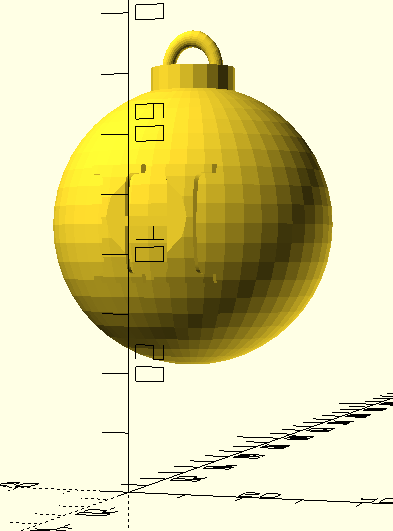
\includegraphics[width=.55\linewidth]{openscad.png}
\caption{Christmas bulb}
\end{figure}

The original file is binary, but re-saving it from OpenSCAD gives us a
more human-readable version:

    \begin{tcolorbox}[breakable, size=fbox, boxrule=1pt, pad at break*=1mm,colback=cellbackground, colframe=cellborder]
\prompt{In}{incolor}{6}{\boxspacing}
\begin{Verbatim}[commandchars=\\\{\}]
\PY{o}{!}head Triangulation2.stl
\end{Verbatim}
\end{tcolorbox}

    \begin{Verbatim}[commandchars=\\\{\}]
solid OpenSCAD\_Model
  facet normal 0.30439 -0.89691 -0.320778
    outer loop
      vertex 11.508 2.34158 36.896
      vertex 11.44 2.30062 36.946
      vertex 9.219 1.794 36.255
    endloop
  endfacet
  facet normal 0.945007 0.0620611 0.321107
    outer loop
    \end{Verbatim}

    \hypertarget{solution}{%
\subsection{Solution}\label{solution}}

I suspected the code was hidden inside the bulb, similar to the Disco
Hacky Easter challenge.

While it'd be possible to find the middle point of the bulb, then write
a script to remove the outside surface, doing so would be quite
cumbersome. Instead, I tried different 3D software to be able to
manipulate the object and ended up using
\href{https://www.prusa3d.com/prusaslicer/}{PrusaSlicer} - that made it
trivial to open the bulb and separate the code:

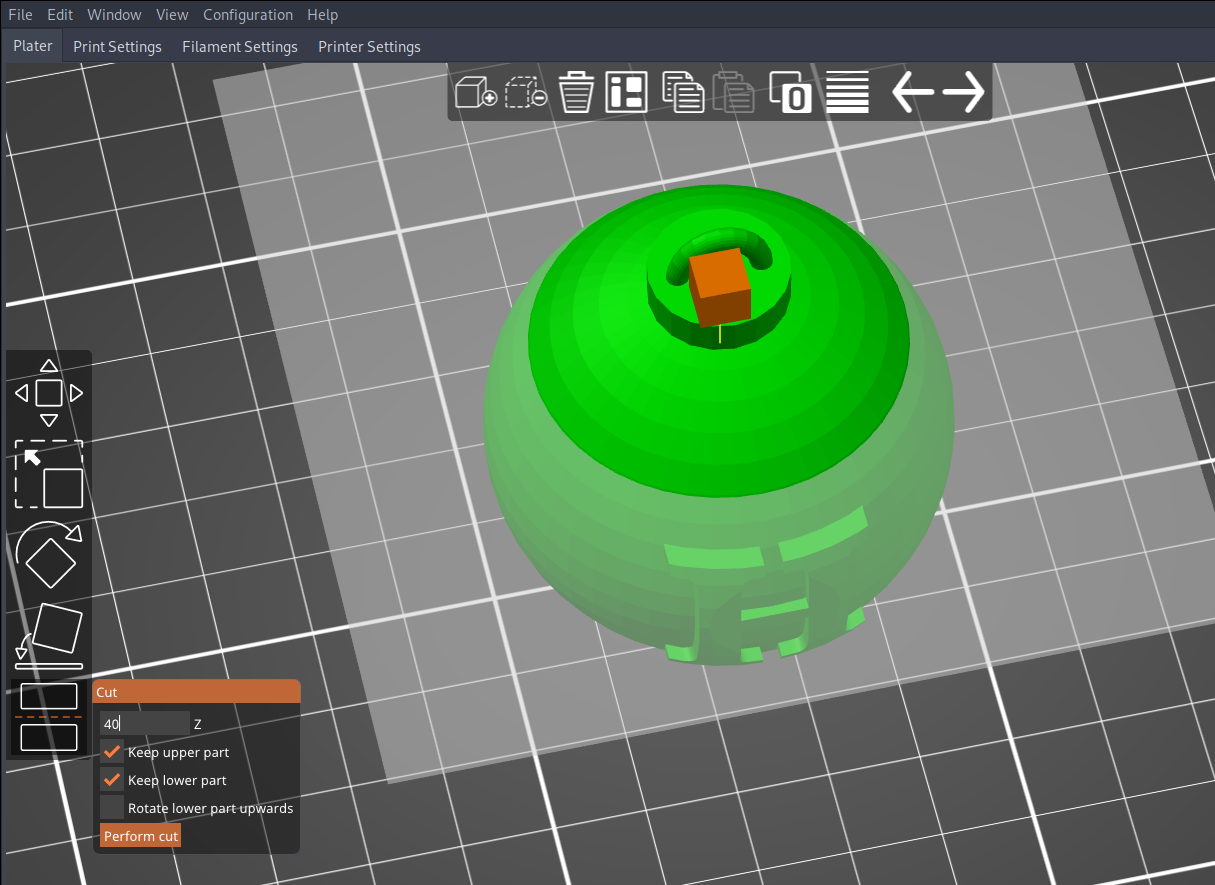
\includegraphics[height=11em]{prusa1.png} 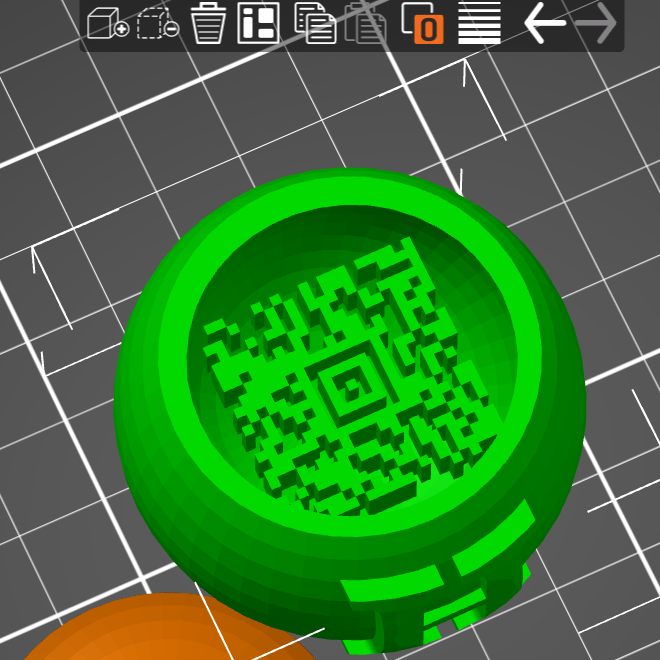
\includegraphics[height=11em]{prusa2.png} 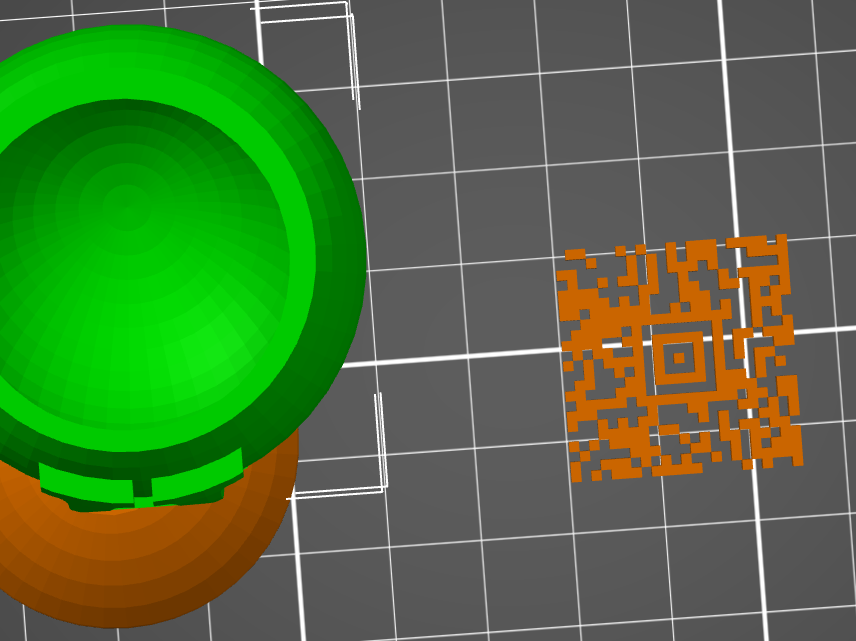
\includegraphics[height=11em]{prusa3.png}

After taking a screenshot, some quick edits in GIMP made the code
readable:

\begin{figure}
\centering

\includegraphics{code.png}
\caption{Code}
\end{figure}

However, note how the code isn't a QR code - it's an
\href{https://en.wikipedia.org/wiki/Aztec_Code}{Aztec Code} instead!

Thankfully, the Android ZXing Barcode Scanner can read those after
enabling them in the settings - which gives us the flag,
\texttt{HV19\{Cr4ck\_Th3\_B411!\}}.


    % Add a bibliography block to the postdoc
    
    
\pagebreak{}
    \hypertarget{hv19.03-hodor-hodor-hodor}{%
\section{HV19.03 Hodor, Hodor, Hodor}\label{hv19.03-hodor-hodor-hodor}}

In this challenge, we get some weird text:

\begin{verbatim}
$HODOR: hhodor. Hodor. Hodor!?  = `hodor?!? HODOR!? hodor? Hodor oHodor.
hodor? , HODOR!?! ohodor!?  dhodor? hodor odhodor? d HodorHodor  Hodor!?
HODOR HODOR? hodor! hodor!? HODOR hodor! hodor? ! 

hodor?!? Hodor  Hodor Hodor? Hodor  HODOR  rhodor? HODOR Hodor!?  h4Hodor?!?
Hodor?!? 0r hhodor?  Hodor!? oHodor?! hodor? Hodor  Hodor! HODOR Hodor hodor?
64 HODOR Hodor  HODOR!? hodor? Hodor!? Hodor!? .

HODOR?!? hodor- hodorHoOodoOor Hodor?!? OHoOodoOorHooodorrHODOR hodor. oHODOR...
Dhodor- hodor?! HooodorrHODOR HoOodoOorHooodorrHODOR RoHODOR... HODOR!?! 1hodor?!
HODOR... DHODOR- HODOR!?! HooodorrHODOR Hodor- HODORHoOodoOor HODOR!?! HODOR...
DHODORHoOodoOor hodor. Hodor! HoOodoOorHodor HODORHoOodoOor 0Hooodorrhodor
HoOodoOorHooodorrHODOR 0=`;
hodor.hod(hhodor. Hodor. Hodor!? );
\end{verbatim}

After spending some quality time with \href{https://duckduckgo.com/}{my
favourite search engine} it was clear that it's the
\href{http://hodor-lang.org/}{Hodor ``programming language''}. A
\texttt{npm\ install\ hodor} later, we can call \texttt{hodor} and get
funny error messages:

    \begin{tcolorbox}[breakable, size=fbox, boxrule=1pt, pad at break*=1mm,colback=cellbackground, colframe=cellborder]
\prompt{In}{incolor}{2}{\boxspacing}
\begin{Verbatim}[commandchars=\\\{\}]
\PY{o}{!}hodor
\end{Verbatim}
\end{tcolorbox}

    \begin{Verbatim}[commandchars=\\\{\}]
\textcolor{ansi-red-intense}{\textbf{HODOR:}}\textcolor{ansi-red}{ hodor hodor hodor!}
    \end{Verbatim}

    But when passing a file, it gets run:

    \begin{tcolorbox}[breakable, size=fbox, boxrule=1pt, pad at break*=1mm,colback=cellbackground, colframe=cellborder]
\prompt{In}{incolor}{3}{\boxspacing}
\begin{Verbatim}[commandchars=\\\{\}]
\PY{o}{!}hodor text.hd
\end{Verbatim}
\end{tcolorbox}

    \begin{Verbatim}[commandchars=\\\{\}]
\textcolor{ansi-cyan-intense}{\textbf{HODOR: }}\textcolor{ansi-white}{\textbackslash{}-> }\textcolor{ansi-white}{text.hd}
Awesome, you decoded Hodors language!

As sis a real h4xx0r he loves base64 as well.

SFYxOXtoMDFkLXRoMy1kMDByLTQyMDQtbGQ0WX0=
    \end{Verbatim}

    All that's left to do is decoding the base64.

    \begin{tcolorbox}[breakable, size=fbox, boxrule=1pt, pad at break*=1mm,colback=cellbackground, colframe=cellborder]
\prompt{In}{incolor}{4}{\boxspacing}
\begin{Verbatim}[commandchars=\\\{\}]
\PY{o}{!}\PY{n+nb}{echo} \PY{l+s+s1}{\PYZsq{}SFYxOXtoMDFkLXRoMy1kMDByLTQyMDQtbGQ0WX0=\PYZsq{}} \PY{p}{|} base64 \PYZhy{}d
\end{Verbatim}
\end{tcolorbox}

    \begin{Verbatim}[commandchars=\\\{\}]
HV19\{h01d-th3-d00r-4204-ld4Y\}
    \end{Verbatim}
    
\pagebreak{}
    \hypertarget{hv19.04-password-policy-circumvention}{%
\section{HV19.04 password policy
circumvention}\label{hv19.04-password-policy-circumvention}}

We get a little story and a .ahk
(\href{https://www.autohotkey.com/}{AutoHotkey}) file.

\emph{Santa released a new password policy (more than 40 characters,
upper, lower, digit, special).}

\emph{The elves can't remember such long passwords, so they found a way
to continue to use their old (bad) password:}

\texttt{merry\ christmas\ geeks}

    When we set up AutoHotkey with that file and type ``merry christmas
geeks'' in a text editor (taking care that we don't type it too fast),
we end up with a flag,
\texttt{HV19\{R3memb3r,\ rem3mber\ -\ the\ 24th\ 0f\ December\}}.

    
\pagebreak{}
    \hypertarget{hv19.05-santa-parcel-tracking}{%
\section{HV19.05 Santa Parcel
Tracking}\label{hv19.05-santa-parcel-tracking}}

\emph{To handle the huge load of parcels Santa introduced this year a
parcel tracking system. He didn't like the black and white barcode, so
he invented a more solemn barcode. Unfortunately the common barcode
readers can't read it anymore, it only works with the pimped models
santa owns. Can you read the barcode}

We get this colored Barcode:

\begin{figure}
\centering

\includegraphics{./barcode.png}
\caption{Barcode}
\end{figure}

Let's read it into Pillow and look at the data.

    \begin{tcolorbox}[breakable, size=fbox, boxrule=1pt, pad at break*=1mm,colback=cellbackground, colframe=cellborder]
\prompt{In}{incolor}{3}{\boxspacing}
\begin{Verbatim}[commandchars=\\\{\}]
\PY{k+kn}{from} \PY{n+nn}{PIL} \PY{k+kn}{import} \PY{n}{Image}

\PY{k}{def} \PY{n+nf}{chunk}\PY{p}{(}\PY{n}{elems}\PY{p}{,} \PY{n}{n}\PY{p}{)}\PY{p}{:}
    \PY{k}{for} \PY{n}{i} \PY{o+ow}{in} \PY{n+nb}{range}\PY{p}{(}\PY{l+m+mi}{0}\PY{p}{,} \PY{n+nb}{len}\PY{p}{(}\PY{n}{elems}\PY{p}{)}\PY{p}{,} \PY{n}{n}\PY{p}{)}\PY{p}{:}
        \PY{k}{yield} \PY{n}{elems}\PY{p}{[}\PY{n}{i}\PY{p}{:}\PY{n}{i} \PY{o}{+} \PY{n}{n}\PY{p}{]}

\PY{k}{def} \PY{n+nf}{load}\PY{p}{(}\PY{p}{)}\PY{p}{:}
    \PY{n}{img} \PY{o}{=} \PY{n}{Image}\PY{o}{.}\PY{n}{open}\PY{p}{(}\PY{l+s+s2}{\PYZdq{}}\PY{l+s+s2}{barcode.png}\PY{l+s+s2}{\PYZdq{}}\PY{p}{)}
    \PY{n}{data} \PY{o}{=} \PY{n+nb}{list}\PY{p}{(}\PY{n}{img}\PY{o}{.}\PY{n}{getdata}\PY{p}{(}\PY{p}{)}\PY{p}{)}

    \PY{c+c1}{\PYZsh{} Split the data into individual lines and only take the first 90 ones (which is the actual code in the image).}
    \PY{c+c1}{\PYZsh{} Then, make sure all lines are the same, so there are no color variations inside the bar.}
    \PY{c+c1}{\PYZsh{} Always a good idea to check if assumptions are correct, especially if it\PYZsq{}s that easy.}
    \PY{n}{lines} \PY{o}{=} \PY{n+nb}{list}\PY{p}{(}\PY{n}{chunk}\PY{p}{(}\PY{n}{data}\PY{p}{,} \PY{n}{img}\PY{o}{.}\PY{n}{width}\PY{p}{)}\PY{p}{)}\PY{p}{[}\PY{p}{:}\PY{l+m+mi}{90}\PY{p}{]}
    \PY{k}{assert} \PY{n+nb}{all}\PY{p}{(}\PY{n}{line} \PY{o}{==} \PY{n}{lines}\PY{p}{[}\PY{l+m+mi}{0}\PY{p}{]} \PY{k}{for} \PY{n}{line} \PY{o+ow}{in} \PY{n}{lines}\PY{p}{)}

    \PY{n}{line} \PY{o}{=} \PY{n}{lines}\PY{p}{[}\PY{l+m+mi}{0}\PY{p}{]}
    
    \PY{c+c1}{\PYZsh{} Here we (ab)use the fact that dictionaries are ordered in Python 3.6+.}
    \PY{c+c1}{\PYZsh{} We want to get the colors of each bar, but eliminate duplicates and ignore while pixels.}
    \PY{n}{colors} \PY{o}{=} \PY{n+nb}{list}\PY{p}{(}\PY{p}{\PYZob{}}\PY{n}{pixel}\PY{p}{:} \PY{k+kc}{None} \PY{k}{for} \PY{n}{pixel} \PY{o+ow}{in} \PY{n}{line} \PY{k}{if} \PY{n}{pixel} \PY{o}{!=} \PY{p}{(}\PY{l+m+mi}{255}\PY{p}{,} \PY{l+m+mi}{255}\PY{p}{,} \PY{l+m+mi}{255}\PY{p}{)}\PY{p}{\PYZcb{}}\PY{p}{)}
    \PY{k}{return} \PY{n}{colors}


\PY{n}{colors} \PY{o}{=} \PY{n}{load}\PY{p}{(}\PY{p}{)}
\PY{n+nb}{print}\PY{p}{(}\PY{n}{colors}\PY{p}{)}
\end{Verbatim}
\end{tcolorbox}

    \begin{Verbatim}[commandchars=\\\{\}]
[(115, 80, 88), (116, 89, 56), (108, 80, 89), (109, 69, 73), (114, 49, 79),
(121, 51, 70), (115, 80, 48), (101, 81, 90), (103, 56, 80), (122, 57, 52), (117,
76, 83), (104, 84, 56), (101, 71, 72), (122, 48, 86), (97, 88, 49), (103, 48,
57), (108, 79, 123), (116, 79, 68), (108, 74, 49), (103, 74, 102), (120, 73,
102), (122, 73, 105), (103, 85, 99), (106, 83, 117), (105, 72, 108), (105, 81,
116), (118, 54, 95), (118, 48, 116), (115, 77, 111), (115, 73, 95), (97, 81,
103), (105, 73, 51), (101, 52, 116), (119, 83, 95), (98, 57, 97), (116, 69, 95),
(117, 71, 83), (104, 52, 80), (97, 56, 84), (108, 78, 95), (113, 86, 82), (99,
86, 51), (108, 80, 97), (102, 54, 100), (113, 53, 101), (114, 71, 114), (99, 79,
125), (119, 88, 83), (102, 76, 49), (113, 48, 48), (118, 86, 57), (101, 87, 48),
(110, 74, 79), (103, 87, 77), (120, 50, 90), (101, 51, 69), (107, 50, 48), (111,
51, 69), (97, 83, 51), (108, 82, 78), (116, 85, 70), (121, 56, 80), (118, 66,
54), (101, 66, 69)]
    \end{Verbatim}

    Note how all values are \textless{} 128 (which is why the barcode is
relatively dark), so the values could be ASCII values? Let's try:

    \begin{tcolorbox}[breakable, size=fbox, boxrule=1pt, pad at break*=1mm,colback=cellbackground, colframe=cellborder]
\prompt{In}{incolor}{5}{\boxspacing}
\begin{Verbatim}[commandchars=\\\{\}]
\PY{n+nb}{print}\PY{p}{(}\PY{l+s+s1}{\PYZsq{}}\PY{l+s+s1}{\PYZsq{}}\PY{o}{.}\PY{n}{join}\PY{p}{(}\PY{n+nb}{chr}\PY{p}{(}\PY{n}{c}\PY{p}{[}\PY{l+m+mi}{0}\PY{p}{]}\PY{p}{)} \PY{k}{for} \PY{n}{c} \PY{o+ow}{in} \PY{n}{colors}\PY{p}{)}\PY{p}{)}  \PY{c+c1}{\PYZsh{} red}
\end{Verbatim}
\end{tcolorbox}

    \begin{Verbatim}[commandchars=\\\{\}]
stlmrysegzuhezagltlgxzgjiivvssaiewbtuhalqclfqrcwfqvengxekoaltyve
    \end{Verbatim}

    \begin{tcolorbox}[breakable, size=fbox, boxrule=1pt, pad at break*=1mm,colback=cellbackground, colframe=cellborder]
\prompt{In}{incolor}{6}{\boxspacing}
\begin{Verbatim}[commandchars=\\\{\}]
\PY{n+nb}{print}\PY{p}{(}\PY{l+s+s1}{\PYZsq{}}\PY{l+s+s1}{\PYZsq{}}\PY{o}{.}\PY{n}{join}\PY{p}{(}\PY{n+nb}{chr}\PY{p}{(}\PY{n}{c}\PY{p}{[}\PY{l+m+mi}{1}\PY{p}{]}\PY{p}{)} \PY{k}{for} \PY{n}{c} \PY{o+ow}{in} \PY{n}{colors}\PY{p}{)}\PY{p}{)}  \PY{c+c1}{\PYZsh{} green}
\end{Verbatim}
\end{tcolorbox}

    \begin{Verbatim}[commandchars=\\\{\}]
PYPE13PQ89LTG0X0OOJJIIUSHQ60MIQI4S9EG48NVVP65GOXL0VWJW2323SRU8BB
    \end{Verbatim}

    \begin{tcolorbox}[breakable, size=fbox, boxrule=1pt, pad at break*=1mm,colback=cellbackground, colframe=cellborder]
\prompt{In}{incolor}{7}{\boxspacing}
\begin{Verbatim}[commandchars=\\\{\}]
\PY{n+nb}{print}\PY{p}{(}\PY{l+s+s1}{\PYZsq{}}\PY{l+s+s1}{\PYZsq{}}\PY{o}{.}\PY{n}{join}\PY{p}{(}\PY{n+nb}{chr}\PY{p}{(}\PY{n}{c}\PY{p}{[}\PY{l+m+mi}{2}\PY{p}{]}\PY{p}{)} \PY{k}{for} \PY{n}{c} \PY{o+ow}{in} \PY{n}{colors}\PY{p}{)}\PY{p}{)}  \PY{c+c1}{\PYZsh{} blue}
\end{Verbatim}
\end{tcolorbox}

    \begin{Verbatim}[commandchars=\\\{\}]
X8YIOF0ZP4S8HV19\{D1fficult\_to\_g3t\_a\_SPT\_R3ader\}S1090OMZE0E3NFP6E
    \end{Verbatim}

    There's our flag, \texttt{HV19\{D1fficult\_to\_g3t\_a\_SPT\_R3ader\}}.
Note that I tried a lot of other things during the challenge, because I
expected the first bars to be \texttt{HV19\{} and didn't look at the
rest of the data\ldots{} Lesson learned: Always question your initial
assumptions.


    
\pagebreak{}
    \hypertarget{hv19.06-bacon-and-eggs}{%
\section{HV19.06 bacon and eggs}\label{hv19.06-bacon-and-eggs}}

We get a text about Francis Bacon which looks kind of weird: Some
letters are italic. Let's feed it to
\href{https://www.crummy.com/software/BeautifulSoup/}{Beautiful Soup} to
take a look!

    \begin{tcolorbox}[breakable, size=fbox, boxrule=1pt, pad at break*=1mm,colback=cellbackground, colframe=cellborder]
\prompt{In}{incolor}{2}{\boxspacing}
\begin{Verbatim}[commandchars=\\\{\}]
\PY{k+kn}{import} \PY{n+nn}{bs4}

\PY{k}{with} \PY{n+nb}{open}\PY{p}{(}\PY{l+s+s1}{\PYZsq{}}\PY{l+s+s1}{francis.html}\PY{l+s+s1}{\PYZsq{}}\PY{p}{)} \PY{k}{as} \PY{n}{f}\PY{p}{:}
    \PY{n}{soup} \PY{o}{=} \PY{n}{bs4}\PY{o}{.}\PY{n}{BeautifulSoup}\PY{p}{(}\PY{n}{f}\PY{o}{.}\PY{n}{read}\PY{p}{(}\PY{p}{)}\PY{p}{,} \PY{l+s+s1}{\PYZsq{}}\PY{l+s+s1}{html.parser}\PY{l+s+s1}{\PYZsq{}}\PY{p}{)}
\end{Verbatim}
\end{tcolorbox}

    \begin{tcolorbox}[breakable, size=fbox, boxrule=1pt, pad at break*=1mm,colback=cellbackground, colframe=cellborder]
\prompt{In}{incolor}{3}{\boxspacing}
\begin{Verbatim}[commandchars=\\\{\}]
\PY{n+nb}{print}\PY{p}{(}\PY{l+s+s1}{\PYZsq{}}\PY{l+s+s1}{\PYZsq{}}\PY{o}{.}\PY{n}{join}\PY{p}{(}\PY{n}{c}\PY{o}{.}\PY{n}{text} \PY{k}{for} \PY{n}{c} \PY{o+ow}{in} \PY{n}{soup}\PY{o}{.}\PY{n}{p}\PY{o}{.}\PY{n}{contents} \PY{k}{if} \PY{n}{c}\PY{o}{.}\PY{n}{name} \PY{o}{==} \PY{l+s+s1}{\PYZsq{}}\PY{l+s+s1}{em}\PY{l+s+s1}{\PYZsq{}}\PY{p}{)}\PY{p}{)}  \PY{c+c1}{\PYZsh{} All italic letters}
\end{Verbatim}
\end{tcolorbox}

    \begin{Verbatim}[commandchars=\\\{\}]
FnnwsangiospnseahrveatneLdChcelEnldsweredeithelongteeitmnedflenalroutcienrouoBco
asbelthfefiricsHiworgessiliycncknoedgadypncirsgaareflbsvfeesnaestiorttyhergueicu
ldbahiespicalndtilaroaerssmoiieadgveAoughpcadaoutschamhtaioitaoglaticthgneiofton
sbitfci
    \end{Verbatim}

    \begin{tcolorbox}[breakable, size=fbox, boxrule=1pt, pad at break*=1mm,colback=cellbackground, colframe=cellborder]
\prompt{In}{incolor}{4}{\boxspacing}
\begin{Verbatim}[commandchars=\\\{\}]
\PY{n+nb}{print}\PY{p}{(}\PY{l+s+s1}{\PYZsq{}}\PY{l+s+s1}{\PYZsq{}}\PY{o}{.}\PY{n}{join}\PY{p}{(}\PY{n}{c} \PY{k}{for} \PY{n}{c} \PY{o+ow}{in} \PY{n}{soup}\PY{o}{.}\PY{n}{p}\PY{o}{.}\PY{n}{contents} \PY{k}{if} \PY{n}{c}\PY{o}{.}\PY{n}{name} \PY{o+ow}{is} \PY{k+kc}{None}\PY{p}{)}\PY{p}{)}  \PY{c+c1}{\PYZsh{} All other text}
\end{Verbatim}
\end{tcolorbox}

    \begin{Verbatim}[commandchars=\\\{\}]
racis Baco a n Elish phloher ad tatsmn wo sed s Atorey Genral and as or anlor of
gan. Hi orks ar citd w dvepi h scintfic mehod and reai inuti thgh he stific
evltin.
an h en caled e athr o empim. s ks arued for th pobit of sietifi wle bse onl uon
idutve eaonin nd cu oeration o vnt in tur. Mo mpanl,  ad scene co e ceved by us
of a cet a mehodca ppch wheby cientist ai t avod mslin themsels. lthh is raticl
ies ab u  etod, he Bconan methd, dd no have  ln-sing nfluene, e eral dea  he
imprtace and posiily o a septcal methodology makes Bacon the father of the
scientific method. This method was a new rhetorical and theoretical framework
for science, the practical details of which are still central in debates about
science and methodology.
    \end{Verbatim}

    Nothing interesting so far. A bit of research reveals
\href{https://en.wikipedia.org/wiki/Bacon's_cipher}{Bacon's cipher}:

\emph{Bacon's cipher or the Baconian cipher is a method of message
encoding devised by Francis Bacon in 1605. A message is concealed in the
presentation of text, rather than its content.}

Oh, that sounds exactly like what we're looking at! Let's try to convert
our tags into A and B's.

    \begin{tcolorbox}[breakable, size=fbox, boxrule=1pt, pad at break*=1mm,colback=cellbackground, colframe=cellborder]
\prompt{In}{incolor}{7}{\boxspacing}
\begin{Verbatim}[commandchars=\\\{\}]
\PY{k}{def} \PY{n+nf}{convert}\PY{p}{(}\PY{n}{tags}\PY{p}{)}\PY{p}{:}
    \PY{k}{for} \PY{n}{t} \PY{o+ow}{in} \PY{n}{tags}\PY{p}{:}
        \PY{k}{if} \PY{n}{t}\PY{o}{.}\PY{n}{name} \PY{o+ow}{is} \PY{k+kc}{None}\PY{p}{:}  \PY{c+c1}{\PYZsh{} text outside tags}
            \PY{k}{for} \PY{n}{c} \PY{o+ow}{in} \PY{n+nb}{str}\PY{p}{(}\PY{n}{t}\PY{p}{)}\PY{p}{:}
                \PY{k}{yield} \PY{l+s+s1}{\PYZsq{}}\PY{l+s+s1}{A}\PY{l+s+s1}{\PYZsq{}}
        \PY{k}{elif} \PY{n}{t}\PY{o}{.}\PY{n}{name} \PY{o}{==} \PY{l+s+s1}{\PYZsq{}}\PY{l+s+s1}{em}\PY{l+s+s1}{\PYZsq{}}\PY{p}{:}  \PY{c+c1}{\PYZsh{} text inside \PYZlt{}em\PYZgt{} tags}
            \PY{k}{for} \PY{n}{c} \PY{o+ow}{in} \PY{n}{t}\PY{o}{.}\PY{n}{text}\PY{p}{:}
                \PY{k}{yield} \PY{l+s+s1}{\PYZsq{}}\PY{l+s+s1}{B}\PY{l+s+s1}{\PYZsq{}}
        \PY{k}{else}\PY{p}{:}  \PY{c+c1}{\PYZsh{} should never happen, but always good to be sure}
            \PY{k}{raise} \PY{n+ne}{Exception}\PY{p}{(}\PY{n}{t}\PY{o}{.}\PY{n}{name}\PY{p}{)}
\end{Verbatim}
\end{tcolorbox}

    \begin{tcolorbox}[breakable, size=fbox, boxrule=1pt, pad at break*=1mm,colback=cellbackground, colframe=cellborder]
\prompt{In}{incolor}{15}{\boxspacing}
\begin{Verbatim}[commandchars=\\\{\}]
\PY{n}{data} \PY{o}{=} \PY{n+nb}{list}\PY{p}{(}\PY{n}{convert}\PY{p}{(}\PY{n}{soup}\PY{o}{.}\PY{n}{p}\PY{o}{.}\PY{n}{contents}\PY{p}{)}\PY{p}{)}
\PY{n+nb}{print}\PY{p}{(}\PY{l+s+s1}{\PYZsq{}}\PY{l+s+s1}{\PYZsq{}}\PY{o}{.}\PY{n}{join}\PY{p}{(}\PY{n}{data}\PY{p}{)}\PY{p}{)}
\end{Verbatim}
\end{tcolorbox}

    \begin{Verbatim}[commandchars=\\\{\}]
BAABAAAAAAAABABABABAAABBAAAAAAABABBABAAAAABAABAAABAABAAABAAAABBBAABAAAABAABAAAAA
ABAAAAAAAAAAABAABABBAABBABAAAAAABBABAABAAAABABAAAAAAABAABBBAABAAABBBAABAABBAABBA
BABAAAABAABAAAAAABAAAAAAAAAABAABBBAAABBABBAABBAAABBBAAABAAAABBBBAAAAAABAABABAABA
AABABBAAABBABABAAAABAAAABBAABAAABAAABAAAABBBBABAAABBAABBBAAAAABAAAAAAAAAABAAABBB
AABBABAAAAABAABAAAABABBBAABBBAAABAABAAAABAABAAAABAABABAAABAABAAAABABAAAABBBBABAA
BBAABAAAAAAABABABAABAAAABBAAABAAAABBABAABBBAABABAABBAABBBBAAAABAABAAAABBBABAABAB
BAAAAAAAAAABAAAAAABAABABBBBAABBAAABAAABAABABAABBBAAAAABBAAAABAAAAAAAABAAABAABAAA
ABAAABAABBBAABAAAAAAAABBAAABAAABBBAABAAABAABAAABAAABABAAAABBBABABBABABAABAAAABAA
AABAAABAAAAAAABAAAABAAAABAAAAAABAABABABBABAAAABAAAAAABAAABBAABABBAAAABAAAABBABAA
AAAABAAABAAAAAAAAAABABAABBAAABAAAABAAABAAAAAAAAAAAAAAAAAAAAAAAAAAAAAAAAAAAAAAAAA
AAAAAAAAAAAAAAAAAAAAAAAAAAAAAAAAAAAAAAAAAAAAAAAAAAAAAAAAAAAAAAAAAAAAAAAAAAAAAAAA
AAAAAAAAAAAAAAAAAAAAAAAAAAAAAAAAAAAAAAAAAAAAAAAAAAAAAAAAAAAAAAAAAAAAAAAAAAAAAAAA
AAAAAAAAAAAAAAAAAAAAAAAAAA
    \end{Verbatim}

    Now let's write some code to convert that into plain text. In reality I
used an \href{http://rumkin.com/tools/cipher/baconian.php}{online tool}
during the challenge, but it's relatively easy to convert it via Python.

    \begin{tcolorbox}[breakable, size=fbox, boxrule=1pt, pad at break*=1mm,colback=cellbackground, colframe=cellborder]
\prompt{In}{incolor}{11}{\boxspacing}
\begin{Verbatim}[commandchars=\\\{\}]
\PY{k+kn}{import} \PY{n+nn}{string}

\PY{n}{bacon\PYZus{}mapping} \PY{o}{=} \PY{p}{\PYZob{}}\PY{l+s+sa}{f}\PY{l+s+s1}{\PYZsq{}}\PY{l+s+si}{\PYZob{}i:05b\PYZcb{}}\PY{l+s+s1}{\PYZsq{}}\PY{p}{:} \PY{n}{c} \PY{k}{for} \PY{n}{i}\PY{p}{,} \PY{n}{c} \PY{o+ow}{in} \PY{n+nb}{enumerate}\PY{p}{(}\PY{n}{string}\PY{o}{.}\PY{n}{ascii\PYZus{}uppercase}\PY{p}{)}\PY{p}{\PYZcb{}}
\PY{n+nb}{print}\PY{p}{(}\PY{n}{bacon\PYZus{}mapping}\PY{p}{)}

\PY{n}{bacon\PYZus{}mapping} \PY{o}{=} \PY{p}{\PYZob{}}\PY{n}{k}\PY{o}{.}\PY{n}{replace}\PY{p}{(}\PY{l+s+s1}{\PYZsq{}}\PY{l+s+s1}{0}\PY{l+s+s1}{\PYZsq{}}\PY{p}{,} \PY{l+s+s1}{\PYZsq{}}\PY{l+s+s1}{A}\PY{l+s+s1}{\PYZsq{}}\PY{p}{)}\PY{o}{.}\PY{n}{replace}\PY{p}{(}\PY{l+s+s1}{\PYZsq{}}\PY{l+s+s1}{1}\PY{l+s+s1}{\PYZsq{}}\PY{p}{,} \PY{l+s+s1}{\PYZsq{}}\PY{l+s+s1}{B}\PY{l+s+s1}{\PYZsq{}}\PY{p}{)}\PY{p}{:} \PY{n}{v} \PY{k}{for} \PY{n}{k}\PY{p}{,} \PY{n}{v} \PY{o+ow}{in} \PY{n}{bacon\PYZus{}mapping}\PY{o}{.}\PY{n}{items}\PY{p}{(}\PY{p}{)}\PY{p}{\PYZcb{}}
\PY{n+nb}{print}\PY{p}{(}\PY{n}{bacon\PYZus{}mapping}\PY{p}{)}
\end{Verbatim}
\end{tcolorbox}

    \begin{Verbatim}[commandchars=\\\{\}]
\{'00000': 'A', '00001': 'B', '00010': 'C', '00011': 'D', '00100': 'E', '00101':
'F', '00110': 'G', '00111': 'H', '01000': 'I', '01001': 'J', '01010': 'K',
'01011': 'L', '01100': 'M', '01101': 'N', '01110': 'O', '01111': 'P', '10000':
'Q', '10001': 'R', '10010': 'S', '10011': 'T', '10100': 'U', '10101': 'V',
'10110': 'W', '10111': 'X', '11000': 'Y', '11001': 'Z'\}
\{'AAAAA': 'A', 'AAAAB': 'B', 'AAABA': 'C', 'AAABB': 'D', 'AABAA': 'E', 'AABAB':
'F', 'AABBA': 'G', 'AABBB': 'H', 'ABAAA': 'I', 'ABAAB': 'J', 'ABABA': 'K',
'ABABB': 'L', 'ABBAA': 'M', 'ABBAB': 'N', 'ABBBA': 'O', 'ABBBB': 'P', 'BAAAA':
'Q', 'BAAAB': 'R', 'BAABA': 'S', 'BAABB': 'T', 'BABAA': 'U', 'BABAB': 'V',
'BABBA': 'W', 'BABBB': 'X', 'BBAAA': 'Y', 'BBAAB': 'Z'\}
    \end{Verbatim}

    \begin{tcolorbox}[breakable, size=fbox, boxrule=1pt, pad at break*=1mm,colback=cellbackground, colframe=cellborder]
\prompt{In}{incolor}{21}{\boxspacing}
\begin{Verbatim}[commandchars=\\\{\}]
\PY{k}{def} \PY{n+nf}{chunk}\PY{p}{(}\PY{n}{elems}\PY{p}{,} \PY{n}{n}\PY{p}{)}\PY{p}{:}
    \PY{k}{for} \PY{n}{i} \PY{o+ow}{in} \PY{n+nb}{range}\PY{p}{(}\PY{l+m+mi}{0}\PY{p}{,} \PY{n+nb}{len}\PY{p}{(}\PY{n}{elems}\PY{p}{)}\PY{p}{,} \PY{n}{n}\PY{p}{)}\PY{p}{:}
        \PY{k}{yield} \PY{n}{elems}\PY{p}{[}\PY{n}{i}\PY{p}{:}\PY{n}{i} \PY{o}{+} \PY{n}{n}\PY{p}{]}
        

\PY{n}{chunks} \PY{o}{=} \PY{p}{[}\PY{l+s+s1}{\PYZsq{}}\PY{l+s+s1}{\PYZsq{}}\PY{o}{.}\PY{n}{join}\PY{p}{(}\PY{n}{e}\PY{p}{)} \PY{k}{for} \PY{n}{e} \PY{o+ow}{in} \PY{n}{chunk}\PY{p}{(}\PY{n}{data}\PY{p}{,} \PY{l+m+mi}{5}\PY{p}{)}\PY{p}{]}
\PY{n+nb}{print}\PY{p}{(}\PY{n}{chunks}\PY{p}{)}
\end{Verbatim}
\end{tcolorbox}

    \begin{Verbatim}[commandchars=\\\{\}]
['BAABA', 'AAAAA', 'AABAB', 'ABABA', 'AABBA', 'AAAAA', 'ABABB', 'ABAAA',
'AABAA', 'BAAAB', 'AABAA', 'ABAAA', 'ABBBA', 'ABAAA', 'ABAAB', 'AAAAA', 'ABAAA',
'AAAAA', 'AAABA', 'ABABB', 'AABBA', 'BAAAA', 'AABBA', 'BAABA', 'AAABA', 'BAAAA',
'AAABA', 'ABBBA', 'ABAAA', 'BBBAA', 'BAABB', 'AABBA', 'BABAA', 'AABAA', 'BAAAA',
'AABAA', 'AAAAA', 'AAABA', 'ABBBA', 'AABBA', 'BBAAB', 'BAAAB', 'BBAAA', 'BAAAA',
'BBBBA', 'AAAAA', 'BAABA', 'BAABA', 'AABAB', 'BAAAB', 'BABAB', 'AAAAB', 'AAAAB',
'BAABA', 'AABAA', 'ABAAA', 'ABBBB', 'ABAAA', 'BBAAB', 'BBAAA', 'AABAA', 'AAAAA',
'AAABA', 'AABBB', 'AABBA', 'BAAAA', 'ABAAB', 'AAAAB', 'ABBBA', 'ABBBA', 'AABAA',
'BAAAA', 'BAABA', 'AAABA', 'ABABA', 'AABAA', 'BAAAA', 'BABAA', 'AABBB', 'BABAA',
'BBAAB', 'AAAAA', 'AABAB', 'ABAAB', 'AAAAB', 'BAAAB', 'AAAAB', 'BABAA', 'BBBAA',
'BABAA', 'BBAAB', 'BBBAA', 'AABAA', 'BAAAA', 'BBBAB', 'AABAB', 'BAAAA', 'AAAAA',
'ABAAA', 'AAABA', 'ABABB', 'BBAAB', 'BAAAB', 'AAABA', 'ABABA', 'ABBBA', 'AAAAB',
'BAAAA', 'BAAAA', 'AAAAB', 'AAABA', 'ABAAA', 'ABAAA', 'BAABB', 'BAABA', 'AAAAA',
'AABBA', 'AABAA', 'ABBBA', 'ABAAA', 'BAABA', 'AABAA', 'ABABA', 'AAABB', 'BABAB',
'BABAB', 'AABAA', 'AABAA', 'AABAA', 'ABAAA', 'AAAAB', 'AAAAB', 'AAAAB', 'AAAAA',
'ABAAB', 'ABABB', 'ABAAA', 'ABAAA', 'AAABA', 'AABBA', 'ABABB', 'AAAAB', 'AAAAB',
'BABAA', 'AAAAB', 'AAABA', 'AAAAA', 'AAAAB', 'ABAAB', 'BAAAB', 'AAAAB', 'AAABA',
'AAAAA', 'AAAAA', 'AAAAA', 'AAAAA', 'AAAAA', 'AAAAA', 'AAAAA', 'AAAAA', 'AAAAA',
'AAAAA', 'AAAAA', 'AAAAA', 'AAAAA', 'AAAAA', 'AAAAA', 'AAAAA', 'AAAAA', 'AAAAA',
'AAAAA', 'AAAAA', 'AAAAA', 'AAAAA', 'AAAAA', 'AAAAA', 'AAAAA', 'AAAAA', 'AAAAA',
'AAAAA', 'AAAAA', 'AAAAA', 'AAAAA', 'AAAAA', 'AAAAA', 'AAAAA', 'AAAAA', 'AAAAA',
'AAAAA', 'AAAAA', 'AAAAA', 'AAAAA', 'AAAAA', 'AAAAA', 'AAAAA', 'AAAAA', 'AAAAA',
'A']
    \end{Verbatim}

    \begin{tcolorbox}[breakable, size=fbox, boxrule=1pt, pad at break*=1mm,colback=cellbackground, colframe=cellborder]
\prompt{In}{incolor}{22}{\boxspacing}
\begin{Verbatim}[commandchars=\\\{\}]
\PY{n+nb}{print}\PY{p}{(}\PY{l+s+s1}{\PYZsq{}}\PY{l+s+s1}{\PYZsq{}}\PY{o}{.}\PY{n}{join}\PY{p}{(}\PY{n}{bacon\PYZus{}mapping}\PY{o}{.}\PY{n}{get}\PY{p}{(}\PY{n}{chunk}\PY{p}{,} \PY{l+s+s1}{\PYZsq{}}\PY{l+s+s1}{?}\PY{l+s+s1}{\PYZsq{}}\PY{p}{)} \PY{k}{for} \PY{n}{chunk} \PY{o+ow}{in} \PY{n}{chunks}\PY{p}{)}\PY{p}{)}
\end{Verbatim}
\end{tcolorbox}

    \begin{Verbatim}[commandchars=\\\{\}]
SAFKGALIEREIOIJAIACLGQGSCQCOI?TGUEQEACOGZRYQ?ASSFRVBBSEIPIZYEACHGQJBOOEQSCKEQUHU
ZAFJBRBU?UZ?EQ?FQAICLZRCKOBQQBCIITSAGEOISEKDVVEEEIBBBAJLIICGLBBUBCABJRBCAAAAAAAA
AAAAAAAAAAAAAAAAAAAAAAAAAAAAAAAAAAAAA?
    \end{Verbatim}

    Hmm, that looks bad. There even are some unknown combinations in
there\ldots{} We have spaces in our input, so we probably shouldn't
count those! Let's try again:

    \begin{tcolorbox}[breakable, size=fbox, boxrule=1pt, pad at break*=1mm,colback=cellbackground, colframe=cellborder]
\prompt{In}{incolor}{23}{\boxspacing}
\begin{Verbatim}[commandchars=\\\{\}]
\PY{k}{def} \PY{n+nf}{clean}\PY{p}{(}\PY{n}{s}\PY{p}{)}\PY{p}{:}
    \PY{k}{return} \PY{n}{s}\PY{o}{.}\PY{n}{replace}\PY{p}{(}\PY{l+s+s1}{\PYZsq{}}\PY{l+s+s1}{ }\PY{l+s+s1}{\PYZsq{}}\PY{p}{,} \PY{l+s+s1}{\PYZsq{}}\PY{l+s+s1}{\PYZsq{}}\PY{p}{)}


\PY{k}{def} \PY{n+nf}{convert}\PY{p}{(}\PY{n}{tags}\PY{p}{)}\PY{p}{:}
    \PY{k}{for} \PY{n}{t} \PY{o+ow}{in} \PY{n}{tags}\PY{p}{:}
        \PY{k}{if} \PY{n}{t}\PY{o}{.}\PY{n}{name} \PY{o+ow}{is} \PY{k+kc}{None}\PY{p}{:}  \PY{c+c1}{\PYZsh{} text outside tags}
            \PY{n}{s} \PY{o}{=} \PY{n}{clean}\PY{p}{(}\PY{n+nb}{str}\PY{p}{(}\PY{n}{t}\PY{p}{)}\PY{p}{)}   \PY{c+c1}{\PYZsh{} NEW: cleaning the string here.}
            \PY{k}{for} \PY{n}{c} \PY{o+ow}{in} \PY{n}{s}\PY{p}{:}
                \PY{k}{yield} \PY{l+s+s1}{\PYZsq{}}\PY{l+s+s1}{A}\PY{l+s+s1}{\PYZsq{}}
        \PY{k}{elif} \PY{n}{t}\PY{o}{.}\PY{n}{name} \PY{o}{==} \PY{l+s+s1}{\PYZsq{}}\PY{l+s+s1}{em}\PY{l+s+s1}{\PYZsq{}}\PY{p}{:}  \PY{c+c1}{\PYZsh{} text inside \PYZlt{}em\PYZgt{} tags}
            \PY{k}{for} \PY{n}{c} \PY{o+ow}{in} \PY{n}{clean}\PY{p}{(}\PY{n}{t}\PY{o}{.}\PY{n}{text}\PY{p}{)}\PY{p}{:}  \PY{c+c1}{\PYZsh{} NEW: cleaning the string here.}
                \PY{k}{yield} \PY{l+s+s1}{\PYZsq{}}\PY{l+s+s1}{B}\PY{l+s+s1}{\PYZsq{}}
        \PY{k}{else}\PY{p}{:}  \PY{c+c1}{\PYZsh{} should never happen, but always good to be sure}
            \PY{k}{raise} \PY{n+ne}{Exception}\PY{p}{(}\PY{n}{t}\PY{o}{.}\PY{n}{name}\PY{p}{)}
            
\PY{n}{data} \PY{o}{=} \PY{n+nb}{list}\PY{p}{(}\PY{n}{convert}\PY{p}{(}\PY{n}{soup}\PY{o}{.}\PY{n}{p}\PY{o}{.}\PY{n}{contents}\PY{p}{)}\PY{p}{)}
\PY{n}{chunks} \PY{o}{=} \PY{p}{[}\PY{l+s+s1}{\PYZsq{}}\PY{l+s+s1}{\PYZsq{}}\PY{o}{.}\PY{n}{join}\PY{p}{(}\PY{n}{e}\PY{p}{)} \PY{k}{for} \PY{n}{e} \PY{o+ow}{in} \PY{n}{chunk}\PY{p}{(}\PY{n}{data}\PY{p}{,} \PY{l+m+mi}{5}\PY{p}{)}\PY{p}{]}
\PY{n+nb}{print}\PY{p}{(}\PY{l+s+s1}{\PYZsq{}}\PY{l+s+s1}{\PYZsq{}}\PY{o}{.}\PY{n}{join}\PY{p}{(}\PY{n}{bacon\PYZus{}mapping}\PY{o}{.}\PY{n}{get}\PY{p}{(}\PY{n}{chunk}\PY{p}{,} \PY{l+s+s1}{\PYZsq{}}\PY{l+s+s1}{?}\PY{l+s+s1}{\PYZsq{}}\PY{p}{)} \PY{k}{for} \PY{n}{chunk} \PY{o+ow}{in} \PY{n}{chunks}\PY{p}{)}\PY{p}{)}
\end{Verbatim}
\end{tcolorbox}

    \begin{Verbatim}[commandchars=\\\{\}]
SANTALIKESHISBACONBURQFZHJTUJAQBHGZTSHQJJCZ?ENCI?TOCAE??EQ?OJCRFEQY?WIDJGEOOK?YS
HVQBCL?EJTQYQBFCJZAGI?ERFD?ZCEICEIKWRAJVRDQIQBJSIQAAAAAAAAAAAAAAAAAAAAAAAAAAAAAA
AAAAAAA?
    \end{Verbatim}

    Finally something readable: \emph{Santa likes his bacon}! We're on the
right track, but something still throws us off. Oh, right, sentences
have punctiation marks. Let's try removing \texttt{.} and \texttt{,}
too.

    \begin{tcolorbox}[breakable, size=fbox, boxrule=1pt, pad at break*=1mm,colback=cellbackground, colframe=cellborder]
\prompt{In}{incolor}{24}{\boxspacing}
\begin{Verbatim}[commandchars=\\\{\}]
\PY{k}{def} \PY{n+nf}{clean}\PY{p}{(}\PY{n}{s}\PY{p}{)}\PY{p}{:}
    \PY{k}{for} \PY{n}{c} \PY{o+ow}{in} \PY{p}{[}\PY{l+s+s1}{\PYZsq{}}\PY{l+s+s1}{ }\PY{l+s+s1}{\PYZsq{}}\PY{p}{,} \PY{l+s+s1}{\PYZsq{}}\PY{l+s+s1}{,}\PY{l+s+s1}{\PYZsq{}}\PY{p}{,} \PY{l+s+s1}{\PYZsq{}}\PY{l+s+s1}{.}\PY{l+s+s1}{\PYZsq{}}\PY{p}{]}\PY{p}{:}
        \PY{n}{s} \PY{o}{=} \PY{n}{s}\PY{o}{.}\PY{n}{replace}\PY{p}{(}\PY{n}{c}\PY{p}{,} \PY{l+s+s1}{\PYZsq{}}\PY{l+s+s1}{\PYZsq{}}\PY{p}{)}
    \PY{k}{return} \PY{n}{s}

\PY{n}{data} \PY{o}{=} \PY{n+nb}{list}\PY{p}{(}\PY{n}{convert}\PY{p}{(}\PY{n}{soup}\PY{o}{.}\PY{n}{p}\PY{o}{.}\PY{n}{contents}\PY{p}{)}\PY{p}{)}
\PY{n}{chunks} \PY{o}{=} \PY{p}{[}\PY{l+s+s1}{\PYZsq{}}\PY{l+s+s1}{\PYZsq{}}\PY{o}{.}\PY{n}{join}\PY{p}{(}\PY{n}{e}\PY{p}{)} \PY{k}{for} \PY{n}{e} \PY{o+ow}{in} \PY{n}{chunk}\PY{p}{(}\PY{n}{data}\PY{p}{,} \PY{l+m+mi}{5}\PY{p}{)}\PY{p}{]}
\PY{n+nb}{print}\PY{p}{(}\PY{l+s+s1}{\PYZsq{}}\PY{l+s+s1}{\PYZsq{}}\PY{o}{.}\PY{n}{join}\PY{p}{(}\PY{n}{bacon\PYZus{}mapping}\PY{o}{.}\PY{n}{get}\PY{p}{(}\PY{n}{chunk}\PY{p}{,} \PY{l+s+s1}{\PYZsq{}}\PY{l+s+s1}{?}\PY{l+s+s1}{\PYZsq{}}\PY{p}{)} \PY{k}{for} \PY{n}{chunk} \PY{o+ow}{in} \PY{n}{chunks}\PY{p}{)}\PY{p}{)}
\end{Verbatim}
\end{tcolorbox}

    \begin{Verbatim}[commandchars=\\\{\}]
SANTALIKESHISBACONBUTALSOTHISBACONTHEPASSLHIRUJD??QQBHGREHTSIUJJEGHVSA?JRHHF?YSH
VQBCL?EJTQYQBFCJZAGR?JCKHXSIRAJCCVUIC?YRYEIAUZEIAAAAAAAAAAAAAAAAAAAAAAAAAAAAAAAA
AAAAA?
    \end{Verbatim}

    Arrrgh. We get \emph{Santa likes his bacon but also this bacon the pass}
and then something throws us off again\ldots{} Let's just filter out
everything except characters then.

    \begin{tcolorbox}[breakable, size=fbox, boxrule=1pt, pad at break*=1mm,colback=cellbackground, colframe=cellborder]
\prompt{In}{incolor}{25}{\boxspacing}
\begin{Verbatim}[commandchars=\\\{\}]
\PY{k+kn}{import} \PY{n+nn}{re}

\PY{k}{def} \PY{n+nf}{clean}\PY{p}{(}\PY{n}{s}\PY{p}{)}\PY{p}{:}
    \PY{k}{return} \PY{n}{re}\PY{o}{.}\PY{n}{sub}\PY{p}{(}\PY{l+s+s1}{\PYZsq{}}\PY{l+s+s1}{[\PYZca{}a\PYZhy{}zA\PYZhy{}Z]}\PY{l+s+s1}{\PYZsq{}}\PY{p}{,} \PY{l+s+s1}{\PYZsq{}}\PY{l+s+s1}{\PYZsq{}}\PY{p}{,} \PY{n}{s}\PY{p}{)}


\PY{n}{data} \PY{o}{=} \PY{n+nb}{list}\PY{p}{(}\PY{n}{convert}\PY{p}{(}\PY{n}{soup}\PY{o}{.}\PY{n}{p}\PY{o}{.}\PY{n}{contents}\PY{p}{)}\PY{p}{)}
\PY{n}{chunks} \PY{o}{=} \PY{p}{[}\PY{l+s+s1}{\PYZsq{}}\PY{l+s+s1}{\PYZsq{}}\PY{o}{.}\PY{n}{join}\PY{p}{(}\PY{n}{e}\PY{p}{)} \PY{k}{for} \PY{n}{e} \PY{o+ow}{in} \PY{n}{chunk}\PY{p}{(}\PY{n}{data}\PY{p}{,} \PY{l+m+mi}{5}\PY{p}{)}\PY{p}{]}
\PY{n+nb}{print}\PY{p}{(}\PY{l+s+s1}{\PYZsq{}}\PY{l+s+s1}{\PYZsq{}}\PY{o}{.}\PY{n}{join}\PY{p}{(}\PY{n}{bacon\PYZus{}mapping}\PY{o}{.}\PY{n}{get}\PY{p}{(}\PY{n}{chunk}\PY{p}{,} \PY{l+s+s1}{\PYZsq{}}\PY{l+s+s1}{?}\PY{l+s+s1}{\PYZsq{}}\PY{p}{)} \PY{k}{for} \PY{n}{chunk} \PY{o+ow}{in} \PY{n}{chunks}\PY{p}{)}\PY{p}{)}
\end{Verbatim}
\end{tcolorbox}

    \begin{Verbatim}[commandchars=\\\{\}]
SANTALIKESHISBACONBUTALSOTHISBACONTHEPASSWORDISHVXBACONCIPHERISSIMPLEBUTCOOLXREP
LACEXWITHBRACKETSANDUSEUPPERCASEFORALLCHARACTERAAAAAAAAAAAAAAAAAAAAAAAAAAAAAAAAA
AAAAA
    \end{Verbatim}

    There we go! \emph{Santa likes his bacon but also this bacon, the
password is ``HVXBACONCIPHERISSIMPLEBUTCOOLX'', replace ``X'' with
brackets and use uppercase for all character.}

That sounds like the flag would be
\texttt{HV\{BACONCIPHERISSIMPLEBUTCOOL\}} - however, that's wrong, as it
should start with \texttt{HV19\{}. After fixing that, the flag is the
correct one.


    
\pagebreak{}
    \hypertarget{hv19.07-santa-rider}{%
\section{HV19.07 Santa Rider}\label{hv19.07-santa-rider}}

\emph{Santa is prototyping a new gadget for his sledge. Unfortunately it
still has some glitches, but look for yourself.}

We get a video with 8 LEDs blinking.

Let's try to get those bytes out of the video! If I had the time and
wanted to learn something new I'd probably have used
\href{https://opencv.org/}{OpenCV} to try and get the data
automatically. However, the video was only 22 seconds long, so I instead
used \texttt{,} and \texttt{.} (frame back/forward) in
\href{https://mpv.io/}{mpv} to get the data by hand. This resulted in:

\begin{verbatim}
01001000
01010110
00110001
00111001
01111011
00110001
01101101
01011111
01100001
01101100
01110011
00110000
01011111
01110111
00110000
01110010
01101011
00110001
01101110
01100111
01011111
00110000
01101110
01011111
01100001
01011111
01110010
00110011
01101101
00110000
01110100
00110011
01011111
01100011
00110000
01101110
01110100
01110000
01101100
01111101
\end{verbatim}

Which looks like a lot like ASCII because the highest bit/LED is always
0. Let's see what Python gives us.

    \begin{tcolorbox}[breakable, size=fbox, boxrule=1pt, pad at break*=1mm,colback=cellbackground, colframe=cellborder]
\prompt{In}{incolor}{1}{\boxspacing}
\begin{Verbatim}[commandchars=\\\{\}]
\PY{k}{with} \PY{n+nb}{open}\PY{p}{(}\PY{l+s+s2}{\PYZdq{}}\PY{l+s+s2}{data.txt}\PY{l+s+s2}{\PYZdq{}}\PY{p}{)} \PY{k}{as} \PY{n}{f}\PY{p}{:}
    \PY{k}{for} \PY{n}{line} \PY{o+ow}{in} \PY{n}{f}\PY{p}{:}
        \PY{n}{c} \PY{o}{=} \PY{n+nb}{chr}\PY{p}{(}\PY{n+nb}{int}\PY{p}{(}\PY{n}{line}\PY{o}{.}\PY{n}{strip}\PY{p}{(}\PY{p}{)}\PY{p}{,} \PY{l+m+mi}{2}\PY{p}{)}\PY{p}{)}
        \PY{n+nb}{print}\PY{p}{(}\PY{n}{c}\PY{p}{,} \PY{n}{end}\PY{o}{=}\PY{l+s+s1}{\PYZsq{}}\PY{l+s+s1}{\PYZsq{}}\PY{p}{)}
\end{Verbatim}
\end{tcolorbox}

    \begin{Verbatim}[commandchars=\\\{\}]
HV19\{1m\_als0\_w0rk1ng\_0n\_a\_r3m0t3\_c0ntpl\}
    \end{Verbatim}

    Looks like I made some mistakes towards the end, but the correct flag
can be easily guessed:
\texttt{HV19\{1m\_als0\_w0rk1ng\_0n\_a\_r3m0t3\_c0ntr0l\}}

    
\pagebreak{}
    \hypertarget{hv19.08-smilencryptor-4.0}{%
\section{HV19.08 SmileNcryptor 4.0}\label{hv19.08-smilencryptor-4.0}}

We get an SQL dump - here are the relevant parts:

\begin{Shaded}
\begin{Highlighting}[]
\KeywordTok{INSERT} \KeywordTok{INTO}\NormalTok{ \textasciigrave{}creditcards\textasciigrave{} }\KeywordTok{VALUES} 
\NormalTok{(}\DecValTok{1}\NormalTok{,}\StringTok{\textquotesingle{}Sirius Black\textquotesingle{}}\NormalTok{,}\StringTok{\textquotesingle{}:)QVXSZUVY\textbackslash{}ZYYZ[a\textquotesingle{}}\NormalTok{,}\StringTok{\textquotesingle{}12/2020\textquotesingle{}}\NormalTok{),}
\NormalTok{(}\DecValTok{2}\NormalTok{,}\StringTok{\textquotesingle{}Hermione Granger\textquotesingle{}}\NormalTok{,}\StringTok{\textquotesingle{}:)QOUW[VT\^{}VY]bZ\_\textquotesingle{}}\NormalTok{,}\StringTok{\textquotesingle{}04/2021\textquotesingle{}}\NormalTok{),}
\NormalTok{(}\DecValTok{3}\NormalTok{,}\StringTok{\textquotesingle{}Draco Malfoy\textquotesingle{}}\NormalTok{,}\StringTok{\textquotesingle{}:)SPPVSSYVV\textbackslash{}YY\_}\CharTok{\textbackslash{}\textbackslash{}}\StringTok{]\textquotesingle{}}\NormalTok{,}\StringTok{\textquotesingle{}05/2020\textquotesingle{}}\NormalTok{),}
\NormalTok{(}\DecValTok{4}\NormalTok{,}\StringTok{\textquotesingle{}Severus Snape\textquotesingle{}}\NormalTok{,}\StringTok{\textquotesingle{}:)RPQRSTUVWXYZ[\textbackslash{}]\^{}\textquotesingle{}}\NormalTok{,}\StringTok{\textquotesingle{}10/2020\textquotesingle{}}\NormalTok{),}
\NormalTok{(}\DecValTok{5}\NormalTok{,}\StringTok{\textquotesingle{}Ron Weasley\textquotesingle{}}\NormalTok{,}\StringTok{\textquotesingle{}:)QTVWRSVUXW[\_Z\textasciigrave{}}\CharTok{\textbackslash{}b}\StringTok{\textquotesingle{}}\NormalTok{,}\StringTok{\textquotesingle{}11/2020\textquotesingle{}}\NormalTok{);}
\end{Highlighting}
\end{Shaded}

\begin{Shaded}
\begin{Highlighting}[]
\KeywordTok{INSERT} \KeywordTok{INTO}\NormalTok{ \textasciigrave{}flags\textasciigrave{} }\KeywordTok{VALUES}\NormalTok{ (}\DecValTok{1}\NormalTok{,}\StringTok{\textquotesingle{}HV19\{\textquotesingle{}}\NormalTok{,}\StringTok{\textquotesingle{}:)SlQRUPXWVo\textbackslash{}Vuv\_n\_}\CharTok{\textbackslash{}a}\StringTok{jjce\textquotesingle{}}\NormalTok{,}\StringTok{\textquotesingle{}\}\textquotesingle{}}\NormalTok{);}
\end{Highlighting}
\end{Shaded}

One weird thing here are the backslashes. When importing this data into
MySQL, they get interpreted, so we end up with invalid data. However,
that's a bug in the challenge. They are meant to be read literally.
First thing which caused some confusion and ended up in me spending way
too much time on this challenge\ldots{}

Either way - let's get the data into Python so we can play with it. For
starters, let's look at the length and character sets. I (correctly)
assumed that \texttt{:)} wasn't part of the actual data, just a marker
for the Smile ``encryption''.

    \begin{tcolorbox}[breakable, size=fbox, boxrule=1pt, pad at break*=1mm,colback=cellbackground, colframe=cellborder]
\prompt{In}{incolor}{2}{\boxspacing}
\begin{Verbatim}[commandchars=\\\{\}]
\PY{n}{ccs} \PY{o}{=} \PY{p}{\PYZob{}}
    \PY{l+s+s1}{\PYZsq{}}\PY{l+s+s1}{sb}\PY{l+s+s1}{\PYZsq{}}\PY{p}{:} \PY{l+s+sa}{r}\PY{l+s+s1}{\PYZsq{}}\PY{l+s+s1}{QVXSZUVY}\PY{l+s+s1}{\PYZbs{}}\PY{l+s+s1}{ZYYZ[a}\PY{l+s+s1}{\PYZsq{}}\PY{p}{,}
    \PY{l+s+s1}{\PYZsq{}}\PY{l+s+s1}{hg}\PY{l+s+s1}{\PYZsq{}}\PY{p}{:} \PY{l+s+sa}{r}\PY{l+s+s1}{\PYZsq{}}\PY{l+s+s1}{QOUW[VT\PYZca{}VY]bZ\PYZus{}}\PY{l+s+s1}{\PYZsq{}}\PY{p}{,}
    \PY{l+s+s1}{\PYZsq{}}\PY{l+s+s1}{dm}\PY{l+s+s1}{\PYZsq{}}\PY{p}{:} \PY{l+s+sa}{r}\PY{l+s+s1}{\PYZsq{}}\PY{l+s+s1}{SPPVSSYVV}\PY{l+s+s1}{\PYZbs{}}\PY{l+s+s1}{YY\PYZus{}}\PY{l+s+se}{\PYZbs{}\PYZbs{}}\PY{l+s+s1}{]}\PY{l+s+s1}{\PYZsq{}}\PY{p}{,}
    \PY{l+s+s1}{\PYZsq{}}\PY{l+s+s1}{ss}\PY{l+s+s1}{\PYZsq{}}\PY{p}{:} \PY{l+s+sa}{r}\PY{l+s+s1}{\PYZsq{}}\PY{l+s+s1}{RPQRSTUVWXYZ[}\PY{l+s+s1}{\PYZbs{}}\PY{l+s+s1}{]\PYZca{}}\PY{l+s+s1}{\PYZsq{}}\PY{p}{,}
    \PY{l+s+s1}{\PYZsq{}}\PY{l+s+s1}{rw}\PY{l+s+s1}{\PYZsq{}}\PY{p}{:} \PY{l+s+sa}{r}\PY{l+s+s1}{\PYZsq{}}\PY{l+s+s1}{QTVWRSVUXW[\PYZus{}Z`}\PY{l+s+s1}{\PYZbs{}}\PY{l+s+s1}{b}\PY{l+s+s1}{\PYZsq{}}\PY{p}{,}
\PY{p}{\PYZcb{}}
\PY{n}{flag} \PY{o}{=} \PY{l+s+sa}{r}\PY{l+s+s1}{\PYZsq{}}\PY{l+s+s1}{SlQRUPXWVo}\PY{l+s+s1}{\PYZbs{}}\PY{l+s+s1}{Vuv\PYZus{}n\PYZus{}}\PY{l+s+s1}{\PYZbs{}}\PY{l+s+s1}{ajjce}\PY{l+s+s1}{\PYZsq{}}
\end{Verbatim}
\end{tcolorbox}

    \begin{tcolorbox}[breakable, size=fbox, boxrule=1pt, pad at break*=1mm,colback=cellbackground, colframe=cellborder]
\prompt{In}{incolor}{11}{\boxspacing}
\begin{Verbatim}[commandchars=\\\{\}]
\PY{n}{ccs\PYZus{}chars} \PY{o}{=} \PY{n+nb}{set}\PY{p}{(}\PY{p}{)}\PY{o}{.}\PY{n}{union}\PY{p}{(}\PY{o}{*}\PY{n}{ccs}\PY{o}{.}\PY{n}{values}\PY{p}{(}\PY{p}{)}\PY{p}{)}
\PY{n+nb}{print}\PY{p}{(}\PY{l+s+sa}{f}\PY{l+s+s2}{\PYZdq{}}\PY{l+s+s2}{credit cards: }\PY{l+s+s2}{\PYZob{}}\PY{l+s+s2}{len(ccs\PYZus{}chars)\PYZcb{} chars: }\PY{l+s+s2}{\PYZob{}}\PY{l+s+s2}{\PYZsq{}}\PY{l+s+s2}{\PYZsq{}}\PY{l+s+s2}{.join(ccs\PYZus{}chars)\PYZcb{}}\PY{l+s+s2}{\PYZdq{}}\PY{p}{)}

\PY{n}{chars} \PY{o}{=} \PY{n+nb}{set}\PY{p}{(}\PY{n}{flag}\PY{p}{)}\PY{o}{.}\PY{n}{union}\PY{p}{(}\PY{o}{*}\PY{n}{ccs}\PY{o}{.}\PY{n}{values}\PY{p}{(}\PY{p}{)}\PY{p}{)}
\PY{n+nb}{print}\PY{p}{(}\PY{l+s+sa}{f}\PY{l+s+s2}{\PYZdq{}}\PY{l+s+s2}{total: }\PY{l+s+s2}{\PYZob{}}\PY{l+s+s2}{len(chars)\PYZcb{} chars: }\PY{l+s+s2}{\PYZob{}}\PY{l+s+s2}{\PYZsq{}}\PY{l+s+s2}{\PYZsq{}}\PY{l+s+s2}{.join(chars)\PYZcb{}}\PY{l+s+s2}{\PYZdq{}}\PY{p}{)}
\end{Verbatim}
\end{tcolorbox}

    \begin{Verbatim}[commandchars=\\\{\}]
credit cards: 20 chars: PR`S\_XVQ[a]T\^{}OZ\textbackslash{}UYbW
total: 28 chars: [PeYR`Sav]T\^{}\_OXjo\textbackslash{}ZulVnQUcbW
    \end{Verbatim}

    \begin{tcolorbox}[breakable, size=fbox, boxrule=1pt, pad at break*=1mm,colback=cellbackground, colframe=cellborder]
\prompt{In}{incolor}{13}{\boxspacing}
\begin{Verbatim}[commandchars=\\\{\}]
\PY{n+nb}{print}\PY{p}{(}\PY{p}{\PYZob{}}\PY{n}{k}\PY{p}{:} \PY{n+nb}{len}\PY{p}{(}\PY{n}{v}\PY{p}{)} \PY{k}{for} \PY{n}{k}\PY{p}{,} \PY{n}{v} \PY{o+ow}{in} \PY{n}{ccs}\PY{o}{.}\PY{n}{items}\PY{p}{(}\PY{p}{)}\PY{p}{\PYZcb{}}\PY{p}{)}
\end{Verbatim}
\end{tcolorbox}

    \begin{Verbatim}[commandchars=\\\{\}]
\{'sb': 15, 'hg': 14, 'dm': 16, 'ss': 16, 'rw': 16\}
    \end{Verbatim}

    Hmm. The length looks like a 1:1 mapping from characters to numbers, but
we have 20 characters for 10 possible digits. Let's see if we can find
out more about how credit card numbers are structured.

From
\href{https://www.creditcardinsider.com/learn/anatomy-of-a-credit-card/}{a
website}, we learn:

\begin{quote}
The first digit is different for each card network: - Visa cards --
Begin with a 4 and have 13 or 16 digits - Mastercard cards -- Begin with
a 5 and has 16 digits - American Express cards -- Begin with a 3,
followed by a 4 or a 7 has 15 digits - Discover cards -- Begin with a 6
and have 16 digits - Diners Club and Carte Blanche cards -- Begin with a
3, followed by a 0, 6, or 8 and have 14 digits
\end{quote}

\emph{Note that Wikipedia has a
\href{https://en.wikipedia.org/wiki/Payment_card_number\#Issuer_identification_number_(IIN)}{more
complete list} which I initially used. I later found out that the data
in the challenge didn't match that list (or
\href{https://www.discovernetwork.com/downloads/IPP_VAR_Compliance.pdf}{Discover's
official compliance document} for Diner's Club) because the 14-digit
number starts with \texttt{30}, but only the \texttt{36}-range is
allowed to have 14 characters. However, the numbers used are
\href{https://www.paypalobjects.com/en_AU/vhelp/paypalmanager_help/credit_card_numbers.htm}{official
test numbers}, so while this confused me and cost me a lot of time, I
can't really blame the authors for that one. Anyways - for the sake of
simplicity I'll use the simplified list.}

Also, there's the
\href{https://en.wikipedia.org/wiki/Luhn_algorithm}{Luhn Algorithm}
which allows validating a credit card number. Let's \sout{implement}
steal it \href{https://stackoverflow.com/a/21079551}{from
stackoverflow}:

    \begin{tcolorbox}[breakable, size=fbox, boxrule=1pt, pad at break*=1mm,colback=cellbackground, colframe=cellborder]
\prompt{In}{incolor}{14}{\boxspacing}
\begin{Verbatim}[commandchars=\\\{\}]
\PY{k}{def} \PY{n+nf}{luhn\PYZus{}checksum}\PY{p}{(}\PY{n}{card\PYZus{}number}\PY{p}{)}\PY{p}{:}
    \PY{k}{def} \PY{n+nf}{digits\PYZus{}of}\PY{p}{(}\PY{n}{n}\PY{p}{)}\PY{p}{:}
        \PY{k}{return} \PY{p}{[}\PY{n+nb}{int}\PY{p}{(}\PY{n}{d}\PY{p}{)} \PY{k}{for} \PY{n}{d} \PY{o+ow}{in} \PY{n+nb}{str}\PY{p}{(}\PY{n}{n}\PY{p}{)}\PY{p}{]}
    \PY{n}{digits} \PY{o}{=} \PY{n}{digits\PYZus{}of}\PY{p}{(}\PY{n}{card\PYZus{}number}\PY{p}{)}
    \PY{n}{odd\PYZus{}digits} \PY{o}{=} \PY{n}{digits}\PY{p}{[}\PY{o}{\PYZhy{}}\PY{l+m+mi}{1}\PY{p}{:}\PY{p}{:}\PY{o}{\PYZhy{}}\PY{l+m+mi}{2}\PY{p}{]}
    \PY{n}{even\PYZus{}digits} \PY{o}{=} \PY{n}{digits}\PY{p}{[}\PY{o}{\PYZhy{}}\PY{l+m+mi}{2}\PY{p}{:}\PY{p}{:}\PY{o}{\PYZhy{}}\PY{l+m+mi}{2}\PY{p}{]}
    \PY{n}{checksum} \PY{o}{=} \PY{l+m+mi}{0}
    \PY{n}{checksum} \PY{o}{+}\PY{o}{=} \PY{n+nb}{sum}\PY{p}{(}\PY{n}{odd\PYZus{}digits}\PY{p}{)}
    \PY{k}{for} \PY{n}{d} \PY{o+ow}{in} \PY{n}{even\PYZus{}digits}\PY{p}{:}
        \PY{n}{checksum} \PY{o}{+}\PY{o}{=} \PY{n+nb}{sum}\PY{p}{(}\PY{n}{digits\PYZus{}of}\PY{p}{(}\PY{n}{d}\PY{o}{*}\PY{l+m+mi}{2}\PY{p}{)}\PY{p}{)}
    \PY{k}{return} \PY{n}{checksum} \PY{o}{\PYZpc{}} \PY{l+m+mi}{10}

\PY{k}{def} \PY{n+nf}{is\PYZus{}luhn\PYZus{}valid}\PY{p}{(}\PY{n}{card\PYZus{}number}\PY{p}{)}\PY{p}{:}
    \PY{k}{return} \PY{n}{luhn\PYZus{}checksum}\PY{p}{(}\PY{n}{card\PYZus{}number}\PY{p}{)} \PY{o}{==} \PY{l+m+mi}{0}
\end{Verbatim}
\end{tcolorbox}

    What information can we infer about the credit card numbers? Based on
the above list, we can infer that:

\begin{itemize}
\tightlist
\item
  Hermione's card is 14 digits long, so her card number starts with
  \texttt{3{[}068{]}}.
\item
  Ron's card is 15 digits long, so it begins with \texttt{3{[}47{]}}.
\end{itemize}

Thus, we can assume that \texttt{Q\ =\ 3} holds. The ascii characters in
the data all are relatively close to each other, so maybe it's just a
simple offset? Let's try!

    \begin{tcolorbox}[breakable, size=fbox, boxrule=1pt, pad at break*=1mm,colback=cellbackground, colframe=cellborder]
\prompt{In}{incolor}{17}{\boxspacing}
\begin{Verbatim}[commandchars=\\\{\}]
\PY{k}{def} \PY{n+nf}{decrypt}\PY{p}{(}\PY{n}{data}\PY{p}{)}\PY{p}{:}
    \PY{n}{diff} \PY{o}{=} \PY{n+nb}{ord}\PY{p}{(}\PY{l+s+s1}{\PYZsq{}}\PY{l+s+s1}{Q}\PY{l+s+s1}{\PYZsq{}}\PY{p}{)} \PY{o}{\PYZhy{}} \PY{n+nb}{ord}\PY{p}{(}\PY{l+s+s1}{\PYZsq{}}\PY{l+s+s1}{3}\PY{l+s+s1}{\PYZsq{}}\PY{p}{)}  \PY{c+c1}{\PYZsh{} 30}
    \PY{n}{decrypted} \PY{o}{=} \PY{p}{[}\PY{n+nb}{chr}\PY{p}{(}\PY{n+nb}{ord}\PY{p}{(}\PY{n}{c}\PY{p}{)} \PY{o}{\PYZhy{}} \PY{n}{diff}\PY{p}{)} \PY{k}{for} \PY{n}{c} \PY{o+ow}{in} \PY{n}{data}\PY{p}{]}
    \PY{k}{return} \PY{l+s+s1}{\PYZsq{}}\PY{l+s+s1}{\PYZsq{}}\PY{o}{.}\PY{n}{join}\PY{p}{(}\PY{n}{decrypted}\PY{p}{)}

\PY{n}{ccs\PYZus{}plain} \PY{o}{=} \PY{p}{\PYZob{}}\PY{n}{k}\PY{p}{:} \PY{n}{decrypt}\PY{p}{(}\PY{n}{v}\PY{p}{)} \PY{k}{for} \PY{n}{k}\PY{p}{,} \PY{n}{v} \PY{o+ow}{in} \PY{n}{ccs}\PY{o}{.}\PY{n}{items}\PY{p}{(}\PY{p}{)}\PY{p}{\PYZcb{}}
\PY{n+nb}{print}\PY{p}{(}\PY{n}{ccs\PYZus{}plain}\PY{p}{)}
\end{Verbatim}
\end{tcolorbox}

    \begin{Verbatim}[commandchars=\\\{\}]
\{'sb': '38:5<78;><;;<=C', 'hg': '3179=86@8;?D<A', 'dm': '522855;88>;;A>>?',
'ss': '423456789:;<=>?@', 'rw': '36894587:9=A<B>D'\}
    \end{Verbatim}

    Nope. After some thinking (and talking to people who solved it) I had an
idea: Maybe it's a
\href{https://en.wikipedia.org/wiki/Polyalphabetic_cipher}{polyalphabetic
cipher}
(e.g.~\href{https://en.wikipedia.org/wiki/Vigen\%C3\%A8re_cipher}{Vigenère})
where the difference shifts with every character? That'd also explain
why the character set of the ciphertext is bigger than the one of the
plaintext.

    \begin{tcolorbox}[breakable, size=fbox, boxrule=1pt, pad at break*=1mm,colback=cellbackground, colframe=cellborder]
\prompt{In}{incolor}{19}{\boxspacing}
\begin{Verbatim}[commandchars=\\\{\}]
\PY{k}{def} \PY{n+nf}{decrypt}\PY{p}{(}\PY{n}{data}\PY{p}{)}\PY{p}{:}
    \PY{n}{diff} \PY{o}{=} \PY{n+nb}{ord}\PY{p}{(}\PY{l+s+s1}{\PYZsq{}}\PY{l+s+s1}{Q}\PY{l+s+s1}{\PYZsq{}}\PY{p}{)} \PY{o}{\PYZhy{}} \PY{n+nb}{ord}\PY{p}{(}\PY{l+s+s1}{\PYZsq{}}\PY{l+s+s1}{3}\PY{l+s+s1}{\PYZsq{}}\PY{p}{)}  \PY{c+c1}{\PYZsh{} 30}
    \PY{n}{decrypted} \PY{o}{=} \PY{p}{[}\PY{n+nb}{chr}\PY{p}{(}\PY{n+nb}{ord}\PY{p}{(}\PY{n}{c}\PY{p}{)} \PY{o}{\PYZhy{}} \PY{n}{diff} \PY{o}{\PYZhy{}} \PY{n}{i}\PY{p}{)} \PY{k}{for} \PY{n}{i}\PY{p}{,} \PY{n}{c} \PY{o+ow}{in} \PY{n+nb}{enumerate}\PY{p}{(}\PY{n}{data}\PY{p}{)}\PY{p}{]}
    \PY{k}{return} \PY{l+s+s1}{\PYZsq{}}\PY{l+s+s1}{\PYZsq{}}\PY{o}{.}\PY{n}{join}\PY{p}{(}\PY{n}{decrypted}\PY{p}{)}

\PY{n}{ccs\PYZus{}plain} \PY{o}{=} \PY{p}{\PYZob{}}\PY{n}{k}\PY{p}{:} \PY{n}{decrypt}\PY{p}{(}\PY{n}{v}\PY{p}{)} \PY{k}{for} \PY{n}{k}\PY{p}{,} \PY{n}{v} \PY{o+ow}{in} \PY{n}{ccs}\PY{o}{.}\PY{n}{items}\PY{p}{(}\PY{p}{)}\PY{p}{\PYZcb{}}
\PY{n+nb}{print}\PY{p}{(}\PY{n}{ccs\PYZus{}plain}\PY{p}{)}
\end{Verbatim}
\end{tcolorbox}

    \begin{Verbatim}[commandchars=\\\{\}]
\{'sb': '378282246310005', 'hg': '30569309025904', 'dm': '5105105105105100',
'ss': '4111111111111111', 'rw': '3566002020360505'\}
    \end{Verbatim}

    Well, that looks promising. Let's say what the Luhn algorithm has to
say!

    \begin{tcolorbox}[breakable, size=fbox, boxrule=1pt, pad at break*=1mm,colback=cellbackground, colframe=cellborder]
\prompt{In}{incolor}{20}{\boxspacing}
\begin{Verbatim}[commandchars=\\\{\}]
\PY{p}{[}\PY{n}{is\PYZus{}luhn\PYZus{}valid}\PY{p}{(}\PY{n}{v}\PY{p}{)} \PY{k}{for} \PY{n}{v} \PY{o+ow}{in} \PY{n}{ccs\PYZus{}plain}\PY{o}{.}\PY{n}{values}\PY{p}{(}\PY{p}{)}\PY{p}{]}
\end{Verbatim}
\end{tcolorbox}

            \begin{tcolorbox}[breakable, size=fbox, boxrule=.5pt, pad at break*=1mm, opacityfill=0]
\prompt{Out}{outcolor}{20}{\boxspacing}
\begin{Verbatim}[commandchars=\\\{\}]
[True, True, True, True, True]
\end{Verbatim}
\end{tcolorbox}
        
    Yay! Final step left: Decrypting the flag.

    \begin{tcolorbox}[breakable, size=fbox, boxrule=1pt, pad at break*=1mm,colback=cellbackground, colframe=cellborder]
\prompt{In}{incolor}{22}{\boxspacing}
\begin{Verbatim}[commandchars=\\\{\}]
\PY{n+nb}{print}\PY{p}{(}\PY{l+s+s1}{\PYZsq{}}\PY{l+s+s1}{HV19}\PY{l+s+s1}{\PYZob{}}\PY{l+s+s1}{\PYZsq{}} \PY{o}{+} \PY{n}{decrypt}\PY{p}{(}\PY{n}{flag}\PY{p}{)} \PY{o}{+} \PY{l+s+s1}{\PYZsq{}}\PY{l+s+s1}{\PYZcb{}}\PY{l+s+s1}{\PYZsq{}}\PY{p}{)}
\end{Verbatim}
\end{tcolorbox}

    \begin{Verbatim}[commandchars=\\\{\}]
HV19\{5M113-420H4-KK3A1-19801\}
    \end{Verbatim}

    Here's another thing which caused this challenge to be much more
frustrating than it should've been: The \texttt{HV19\{...\}} pattern
isn't part of the flag to decrypt, and the flag also isn't really
recognizable as the solution (the only thing I can decipher is ``5M113''
= ``smile''). This kind of thing only makes the challenge needlessly
frustrating, because you might have the solution but not recognize
it\ldots{}


    
\pagebreak{}
    \hypertarget{hv19.09-santas-quick-response-3.0}{%
\section{HV19.09 Santas Quick Response
3.0}\label{hv19.09-santas-quick-response-3.0}}

    \hypertarget{introduction}{%
\subsection{Introduction}\label{introduction}}

We get the following picture of a railway station:

\begin{figure}
\centering
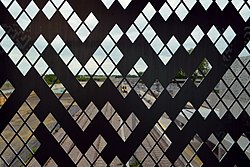
\includegraphics{train.jpg}
\caption{Railway Station}
\end{figure}

And a somewhat broken QR code:

\begin{figure}
\centering

\includegraphics{qr.png}
\caption{QR Code}
\end{figure}

    \hypertarget{initial-research}{%
\subsection{Initial research}\label{initial-research}}

A Google reverse image search reveals a
\href{https://en.wikipedia.org/wiki/Rule_30}{Wikipedia article} about
``Rule 30'', a cellular automaton similar to e.g.~Conway's Game of Life:

\begin{figure}
\centering

\includegraphics{rule30.png}
\caption{Rule 30}
\end{figure}

Pixels are set based on the pattern above them:

\begin{longtable}[]{@{}llllllll@{}}
\toprule
111 & 110 & 101 & 100 & 011 & 010 & 001 & 000\tabularnewline
\midrule
\endhead
0 & 0 & 0 & 1 & 1 & 1 & 1 & 0\tabularnewline
\bottomrule
\end{longtable}

    \hypertarget{loading-qr-code}{%
\subsection{Loading QR code}\label{loading-qr-code}}

First, let's try to load the QR code into Python via
\href{https://pillow.readthedocs.io/}{Pillow}. The QR code is 33x33
squares big, one square is 5x5px.

    \begin{tcolorbox}[breakable, size=fbox, boxrule=1pt, pad at break*=1mm,colback=cellbackground, colframe=cellborder]
\prompt{In}{incolor}{3}{\boxspacing}
\begin{Verbatim}[commandchars=\\\{\}]
\PY{k+kn}{from} \PY{n+nn}{PIL} \PY{k+kn}{import} \PY{n}{Image}

\PY{n}{CNT} \PY{o}{=} \PY{l+m+mi}{33}  \PY{c+c1}{\PYZsh{} squares in the QR\PYZhy{}code}

\PY{k}{def} \PY{n+nf}{read}\PY{p}{(}\PY{p}{)}\PY{p}{:}
    \PY{n}{qr} \PY{o}{=} \PY{n}{Image}\PY{o}{.}\PY{n}{open}\PY{p}{(}\PY{l+s+s2}{\PYZdq{}}\PY{l+s+s2}{qr.png}\PY{l+s+s2}{\PYZdq{}}\PY{p}{)}
    \PY{n}{data} \PY{o}{=} \PY{p}{[}\PY{p}{[}\PY{p}{]} \PY{k}{for} \PY{n}{\PYZus{}} \PY{o+ow}{in} \PY{n+nb}{range}\PY{p}{(}\PY{n}{CNT}\PY{p}{)}\PY{p}{]}
    \PY{k}{for} \PY{n}{sq\PYZus{}y} \PY{o+ow}{in} \PY{n+nb}{range}\PY{p}{(}\PY{n}{CNT}\PY{p}{)}\PY{p}{:}
        \PY{k}{for} \PY{n}{sq\PYZus{}x} \PY{o+ow}{in} \PY{n+nb}{range}\PY{p}{(}\PY{n}{CNT}\PY{p}{)}\PY{p}{:}
            \PY{n}{pixel} \PY{o}{=} \PY{n}{qr}\PY{o}{.}\PY{n}{getpixel}\PY{p}{(}\PY{p}{(}\PY{n}{sq\PYZus{}x} \PY{o}{*} \PY{l+m+mi}{5}\PY{p}{,} \PY{n}{sq\PYZus{}y} \PY{o}{*} \PY{l+m+mi}{5}\PY{p}{)}\PY{p}{)}
            \PY{n}{val} \PY{o}{=} \PY{p}{\PYZob{}}\PY{l+m+mi}{0}\PY{p}{:} \PY{l+m+mi}{1}\PY{p}{,} \PY{l+m+mi}{255}\PY{p}{:} \PY{l+m+mi}{0}\PY{p}{\PYZcb{}}\PY{p}{[}\PY{n}{pixel}\PY{p}{]}
            \PY{n}{data}\PY{p}{[}\PY{n}{sq\PYZus{}y}\PY{p}{]}\PY{o}{.}\PY{n}{append}\PY{p}{(}\PY{n}{val}\PY{p}{)}
        
    \PY{k}{return} \PY{n}{data}

\PY{k}{def} \PY{n+nf}{display}\PY{p}{(}\PY{n}{data}\PY{p}{)}\PY{p}{:}
    \PY{n}{chars} \PY{o}{=} \PY{p}{\PYZob{}}\PY{l+m+mi}{1}\PY{p}{:} \PY{l+s+s1}{\PYZsq{}}\PY{l+s+s1}{*}\PY{l+s+s1}{\PYZsq{}}\PY{p}{,} \PY{l+m+mi}{0}\PY{p}{:} \PY{l+s+s1}{\PYZsq{}}\PY{l+s+s1}{ }\PY{l+s+s1}{\PYZsq{}}\PY{p}{\PYZcb{}}
    \PY{k}{for} \PY{n}{line} \PY{o+ow}{in} \PY{n}{data}\PY{p}{:}
        \PY{n+nb}{print}\PY{p}{(}\PY{l+s+s1}{\PYZsq{}}\PY{l+s+s1}{\PYZsq{}}\PY{o}{.}\PY{n}{join}\PY{p}{(}\PY{n}{chars}\PY{p}{[}\PY{n}{c}\PY{p}{]} \PY{k}{for} \PY{n}{c} \PY{o+ow}{in} \PY{n}{line}\PY{p}{)}\PY{p}{)}
\end{Verbatim}
\end{tcolorbox}

    \begin{tcolorbox}[breakable, size=fbox, boxrule=1pt, pad at break*=1mm,colback=cellbackground, colframe=cellborder]
\prompt{In}{incolor}{4}{\boxspacing}
\begin{Verbatim}[commandchars=\\\{\}]
\PY{n}{data} \PY{o}{=} \PY{n}{read}\PY{p}{(}\PY{p}{)}
\PY{n}{display}\PY{p}{(}\PY{n}{data}\PY{p}{)}
\end{Verbatim}
\end{tcolorbox}

    \begin{Verbatim}[commandchars=\\\{\}]
*******   *  * **   ***   *******
*     * **  ** *****  * * *     *
* *** * ** * *** *****  * * *** *
* *** * **   * * * ****   * *** *
* *** * **** *     **  *  * *** *
*     * ****  ****  ** *  *     *
******* * **  *** *   *** *******
         ***** ** *  **
  *  ****   * *   *     *  *****
  **** ** * *** * *   **       **
* * * **   * * * * ** * ******* *
 *    **  * *     * * ***  ***
    **  *   *  *    **  *** ** **
 ***    ** * * * *     ** * ***
   ** *   *  **     *** ***   ***
 **   * *  *    * * **** ****** *
  *   *    *  **  *      * *  **
****  * **  * *  * *   * **   * *
* *  ****** **  ** *  *  **  ****
*  *   **  * *     *** * ***  ***
 * **   * ***** ***  *  *******
*** *   * **  **  ****  *  *****
*** *    ** **** * ***  *  * * *
* *  ****  ***** * * * * * ******
*  ***  ** *  **  *  *** *    * *
**  *** * ** * *   *   *  * *  *
 *   *****    *** ** * **  ***
  *  * **** *** *    *   **  **
*    **   *   *** *   * **** ****
 * **   ** ** **  * **   *   *  *
  * **     **  * *    *  ** *****
**** ** ***   *  ***  *****    *
  ***  ***    **    ** **  * ** *
    \end{Verbatim}

    \hypertarget{first-idea}{%
\subsection{First idea}\label{first-idea}}

Looking at the QR code, the data in the top corners seems to be valid
(so we probably don't need to touch it), while the data in the bottom
corners clearly isn't a valid QR code. When taking a closer look, we
also see some other patterns that are missing - from Wikipedia:

\begin{figure}
\centering
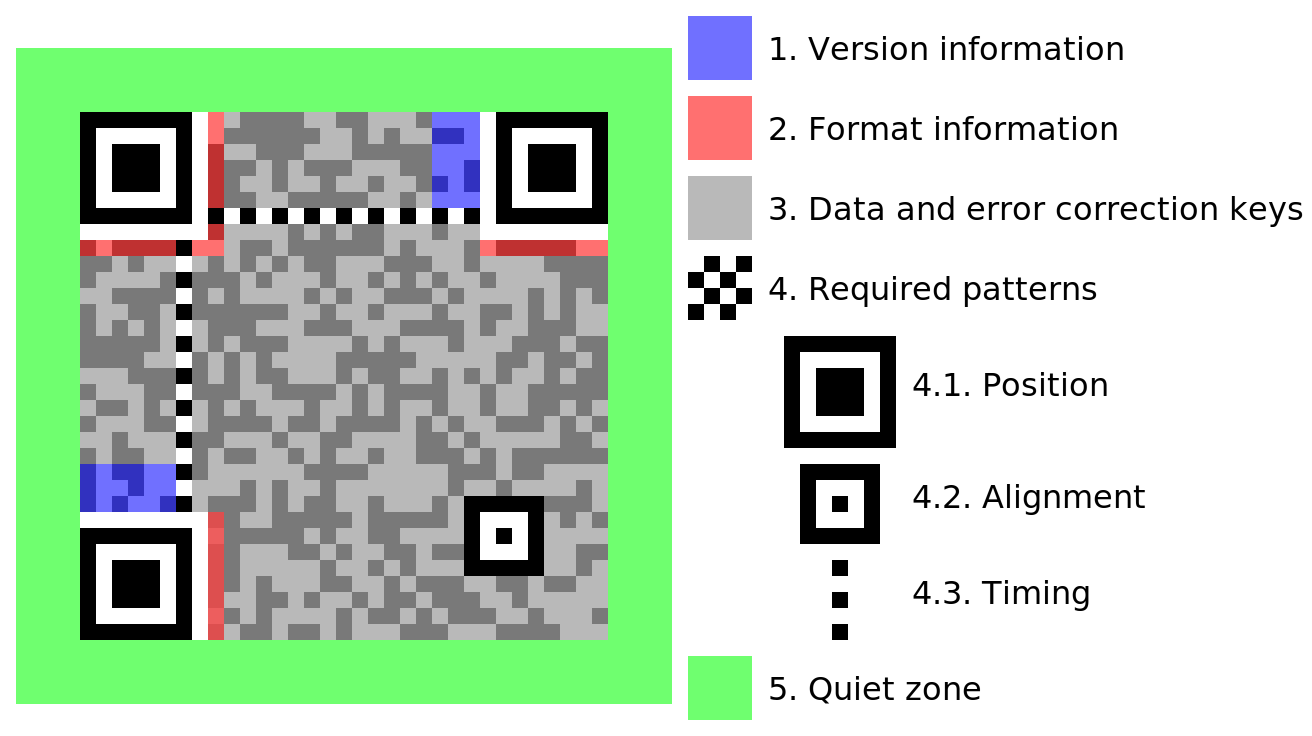
\includegraphics{qr-structure.pdf}
\caption{QR code structure}
\end{figure}

Thus, we maybe need to use the rule30 data to toggle bits, so that we
leave the top corners alone but modify the bottom corners?

I'll use the \href{https://pypi.org/project/rule30/}{rule30} Python
library to generate Rule30 patterns.

    \begin{tcolorbox}[breakable, size=fbox, boxrule=1pt, pad at break*=1mm,colback=cellbackground, colframe=cellborder]
\prompt{In}{incolor}{5}{\boxspacing}
\begin{Verbatim}[commandchars=\\\{\}]
\PY{k+kn}{import} \PY{n+nn}{rule30}

\PY{n}{r30} \PY{o}{=} \PY{n}{rule30}\PY{o}{.}\PY{n}{Automaton}\PY{p}{(}\PY{n}{rows}\PY{o}{=}\PY{n}{CNT}\PY{p}{)}
\PY{n+nb}{print}\PY{p}{(}\PY{n}{r30}\PY{o}{.}\PY{n}{string}\PY{p}{(}\PY{p}{)}\PY{p}{)}
\end{Verbatim}
\end{tcolorbox}

    \begin{Verbatim}[commandchars=\\\{\}]
00000000000000000000000000000000100000000000000000000000000000000
00000000000000000000000000000001110000000000000000000000000000000
00000000000000000000000000000011001000000000000000000000000000000
00000000000000000000000000000110111100000000000000000000000000000
00000000000000000000000000001100100010000000000000000000000000000
00000000000000000000000000011011110111000000000000000000000000000
00000000000000000000000000110010000100100000000000000000000000000
00000000000000000000000001101111001111110000000000000000000000000
00000000000000000000000011001000111000001000000000000000000000000
00000000000000000000000110111101100100011100000000000000000000000
00000000000000000000001100100001011110110010000000000000000000000
00000000000000000000011011110011010000101111000000000000000000000
00000000000000000000110010001110011001101000100000000000000000000
00000000000000000001101111011001110111001101110000000000000000000
00000000000000000011001000010111000100111001001000000000000000000
00000000000000000110111100110100101111100111111100000000000000000
00000000000000001100100011100111101000011100000010000000000000000
00000000000000011011110110011100001100110010000111000000000000000
00000000000000110010000101110010011011101111001100100000000000000
00000000000001101111001101001111110010001000111011110000000000000
00000000000011001000111001111000001111011101100010001000000000000
00000000000110111101100111000100011000010001010111011100000000000
00000000001100100001011100101110110100111011010100010010000000000
00000000011011110011010011101000100111100010010110111111000000000
00000000110010001110011110001101111100010111110100100000100000000
00000001101111011001110001011001000010110100000111110001110000000
00000011001000010111001011010111100110100110001100001011001000000
00000110111100110100111010010100011100111101011010011010111100000
00001100100011100111100011110110110011100001010011110010100010000
00011011110110011100010110000100101110010011011110001110110111000
00110010000101110010110101001111101001111110010001011000100100100
01101111001101001110100101111000001111000001111011010101111111110
11001000111001111000111101000100011000100011000010010101000000001
    \end{Verbatim}

    This looks like something we can use to try that theory, but it's not a
square\ldots{} Given that the QR code is 33x33 fields big, you'd think
you can just start with the middle pixel in the first row. This doesn't
result in a working QR code however.

After my original (failed) approach, I fired up GIMP and tried to create
a ``diff'' of what you'd need to change in the QR code to get the fixed
patterns. Dark read means ``is 0 but should be 1'', light red means ``is
1 but should be 0''.

\begin{figure}
\centering

\includegraphics{qr-diff.png}
\caption{QR code diff}
\end{figure}

I couldn't find those patterns in rule30, so I might have done a mistake
at some point. However, it later turned out that the start is shifted by
one pixel\ldots{} A challenge hint ``centering is hard'' was released
later, but I'm assuming this wasn't originally intended.

    \begin{tcolorbox}[breakable, size=fbox, boxrule=1pt, pad at break*=1mm,colback=cellbackground, colframe=cellborder]
\prompt{In}{incolor}{6}{\boxspacing}
\begin{Verbatim}[commandchars=\\\{\}]
\PY{n+nb}{len}\PY{p}{(}\PY{n}{r30}\PY{o}{.}\PY{n}{matrix}\PY{p}{[}\PY{l+m+mi}{0}\PY{p}{]}\PY{p}{)}\PY{p}{,} \PY{n+nb}{len}\PY{p}{(}\PY{n}{r30}\PY{o}{.}\PY{n}{matrix}\PY{p}{)}  \PY{c+c1}{\PYZsh{} width, height}
\end{Verbatim}
\end{tcolorbox}

            \begin{tcolorbox}[breakable, size=fbox, boxrule=.5pt, pad at break*=1mm, opacityfill=0]
\prompt{Out}{outcolor}{6}{\boxspacing}
\begin{Verbatim}[commandchars=\\\{\}]
(65, 33)
\end{Verbatim}
\end{tcolorbox}
        
    \begin{tcolorbox}[breakable, size=fbox, boxrule=1pt, pad at break*=1mm,colback=cellbackground, colframe=cellborder]
\prompt{In}{incolor}{7}{\boxspacing}
\begin{Verbatim}[commandchars=\\\{\}]
\PY{k}{def} \PY{n+nf}{flip\PYZus{}bits}\PY{p}{(}\PY{n}{data}\PY{p}{)}\PY{p}{:}
    \PY{n}{diff} \PY{o}{=} \PY{l+m+mi}{65} \PY{o}{\PYZhy{}} \PY{n}{CNT}
    \PY{c+c1}{\PYZsh{} For some reason, it\PYZsq{}s not centered in the challenge...}
    \PY{n}{left} \PY{o}{=} \PY{n}{diff} \PY{o}{/}\PY{o}{/} \PY{l+m+mi}{2} \PY{o}{\PYZhy{}} \PY{l+m+mi}{1}
    \PY{n}{right} \PY{o}{=} \PY{n}{diff} \PY{o}{/}\PY{o}{/} \PY{l+m+mi}{2} \PY{o}{+} \PY{l+m+mi}{1}
    \PY{k}{for} \PY{n}{y} \PY{o+ow}{in} \PY{n+nb}{range}\PY{p}{(}\PY{n}{CNT}\PY{p}{)}\PY{p}{:}
        \PY{n}{r30\PYZus{}line} \PY{o}{=} \PY{n}{r30}\PY{o}{.}\PY{n}{matrix}\PY{p}{[}\PY{n}{y}\PY{p}{]}\PY{p}{[}\PY{n}{left}\PY{p}{:}\PY{o}{\PYZhy{}}\PY{n}{right}\PY{p}{]}
        \PY{c+c1}{\PYZsh{} print(r30\PYZus{}line)}
        \PY{k}{for} \PY{n}{x} \PY{o+ow}{in} \PY{n+nb}{range}\PY{p}{(}\PY{n}{CNT}\PY{p}{)}\PY{p}{:}
            \PY{n}{data}\PY{p}{[}\PY{n}{y}\PY{p}{]}\PY{p}{[}\PY{n}{x}\PY{p}{]} \PY{o}{\PYZca{}}\PY{o}{=} \PY{n}{r30\PYZus{}line}\PY{p}{[}\PY{n}{x}\PY{p}{]}
\end{Verbatim}
\end{tcolorbox}

    \begin{tcolorbox}[breakable, size=fbox, boxrule=1pt, pad at break*=1mm,colback=cellbackground, colframe=cellborder]
\prompt{In}{incolor}{8}{\boxspacing}
\begin{Verbatim}[commandchars=\\\{\}]
\PY{n}{data} \PY{o}{=} \PY{n}{read}\PY{p}{(}\PY{p}{)}
\PY{n}{flip\PYZus{}bits}\PY{p}{(}\PY{n}{data}\PY{p}{)}
\end{Verbatim}
\end{tcolorbox}

    This results in something which looks like a QR-code!

    \begin{tcolorbox}[breakable, size=fbox, boxrule=1pt, pad at break*=1mm,colback=cellbackground, colframe=cellborder]
\prompt{In}{incolor}{9}{\boxspacing}
\begin{Verbatim}[commandchars=\\\{\}]
\PY{n}{display}\PY{p}{(}\PY{n}{data}\PY{p}{)}
\end{Verbatim}
\end{tcolorbox}

    \begin{Verbatim}[commandchars=\\\{\}]
*******   *  * ***  ***   *******
*     * **  ** *   *  * * *     *
* *** * ** * ** *** **  * * *** *
* *** * **   **   *  **   * *** *
* *** * ****  *  * *** *  * *** *
*     * *******   *   **  *     *
******* * * * * * * * * * *******
         *  * *   ***  **
  *  ****** ***  * *    ** *****
  **** * ***     ** * *****    **
* * * * *    * ****  *** ** *** *
 *       * *   **   * * ***  *
    * * **  ***   ******* * *  **
 ***** *  ***  ** * ******
      **  * ** **    ***  * * * *
 * * * *    * * ****     *     *
 *   **  **     ****    * **  **
  * **       *   *  *   ****  *
  ** *** * * * ****  * *   ****
*** *     **  *******  *  ** *  *
   ******     * ***** *    *  *
     *   * *   *    **     * * **
***   *******     ** * * *  *****
  **** **** * **   ** *  *  ** *
*** ****   * * *** ***********
        *  **  **  * *  *   *  **
******* * * *    ****   * * ** **
*     * * *  *  * **** **   ** *
* *** *  * **   **   * ******* **
* *** *    **  * ***    ** *****
* *** * * ***** *  *   **  *** **
*     *  * ****  ** ** **** ***
*******  **    *  ****  *   *** *
    \end{Verbatim}

    \begin{tcolorbox}[breakable, size=fbox, boxrule=1pt, pad at break*=1mm,colback=cellbackground, colframe=cellborder]
\prompt{In}{incolor}{13}{\boxspacing}
\begin{Verbatim}[commandchars=\\\{\}]
\PY{k+kn}{import} \PY{n+nn}{itertools}

\PY{k}{def} \PY{n+nf}{write\PYZus{}img}\PY{p}{(}\PY{n}{data}\PY{p}{)}\PY{p}{:}
    \PY{n}{img} \PY{o}{=} \PY{n}{Image}\PY{o}{.}\PY{n}{new}\PY{p}{(}\PY{n}{mode}\PY{o}{=}\PY{l+s+s1}{\PYZsq{}}\PY{l+s+s1}{1}\PY{l+s+s1}{\PYZsq{}}\PY{p}{,} \PY{n}{size}\PY{o}{=}\PY{p}{(}\PY{n}{CNT}\PY{p}{,} \PY{n}{CNT}\PY{p}{)}\PY{p}{)}
    \PY{k}{for} \PY{n}{y}\PY{p}{,} \PY{n}{line} \PY{o+ow}{in} \PY{n+nb}{enumerate}\PY{p}{(}\PY{n}{data}\PY{p}{)}\PY{p}{:}
        \PY{k}{for} \PY{n}{x}\PY{p}{,} \PY{n}{val} \PY{o+ow}{in} \PY{n+nb}{enumerate}\PY{p}{(}\PY{n}{line}\PY{p}{)}\PY{p}{:}
            \PY{n}{img}\PY{o}{.}\PY{n}{putpixel}\PY{p}{(}\PY{p}{(}\PY{n}{x}\PY{p}{,} \PY{n}{y}\PY{p}{)}\PY{p}{,} \PY{o+ow}{not} \PY{n}{val}\PY{p}{)}
    
    \PY{k}{return} \PY{n}{img}\PY{o}{.}\PY{n}{resize}\PY{p}{(}\PY{p}{(}\PY{n}{CNT} \PY{o}{*} \PY{l+m+mi}{5}\PY{p}{,} \PY{n}{CNT} \PY{o}{*} \PY{l+m+mi}{5}\PY{p}{)}\PY{p}{)}

\PY{n}{img} \PY{o}{=} \PY{n}{write\PYZus{}img}\PY{p}{(}\PY{n}{data}\PY{p}{)}
\PY{n}{img}\PY{o}{.}\PY{n}{save}\PY{p}{(}\PY{l+s+s2}{\PYZdq{}}\PY{l+s+s2}{result.png}\PY{l+s+s2}{\PYZdq{}}\PY{p}{)}
\end{Verbatim}
\end{tcolorbox}

    This gives us the QR code. For some extra h4xx0r points, let's use
\href{https://github.com/Polyconseil/zbarlight/}{zbarlight} to get the
flag as well.

    \begin{figure}
\centering

\includegraphics{result.png}
\caption{Resulting QR-Code}
\end{figure}

    \begin{tcolorbox}[breakable, size=fbox, boxrule=1pt, pad at break*=1mm,colback=cellbackground, colframe=cellborder]
\prompt{In}{incolor}{14}{\boxspacing}
\begin{Verbatim}[commandchars=\\\{\}]
\PY{k+kn}{import} \PY{n+nn}{zbarlight}
    
\PY{n}{codes} \PY{o}{=} \PY{n}{zbarlight}\PY{o}{.}\PY{n}{scan\PYZus{}codes}\PY{p}{(}\PY{p}{[}\PY{l+s+s1}{\PYZsq{}}\PY{l+s+s1}{qrcode}\PY{l+s+s1}{\PYZsq{}}\PY{p}{]}\PY{p}{,} \PY{n}{img}\PY{p}{)}
\PY{n+nb}{print}\PY{p}{(}\PY{n}{codes}\PY{p}{[}\PY{l+m+mi}{0}\PY{p}{]}\PY{o}{.}\PY{n}{decode}\PY{p}{(}\PY{l+s+s1}{\PYZsq{}}\PY{l+s+s1}{ascii}\PY{l+s+s1}{\PYZsq{}}\PY{p}{)}\PY{p}{)}
\end{Verbatim}
\end{tcolorbox}

    \begin{Verbatim}[commandchars=\\\{\}]
HV19\{Cha0tic\_yet-0rdered\}
    \end{Verbatim}


    
\pagebreak{}
    \hypertarget{hv19.10-guess-what}{%
\section{HV19.10 Guess what}\label{hv19.10-guess-what}}

With the new (v3) fixed binary, this was easy - I suspect there would be
a harder ``proper'' solution, maybe?

Running the binary asks for an input:

    \begin{tcolorbox}[breakable, size=fbox, boxrule=1pt, pad at break*=1mm,colback=cellbackground, colframe=cellborder]
\prompt{In}{incolor}{1}{\boxspacing}
\begin{Verbatim}[commandchars=\\\{\}]
\PY{o}{!}./guess3
\end{Verbatim}
\end{tcolorbox}

    \begin{Verbatim}[commandchars=\\\{\}]
Your input:
    \end{Verbatim}

    With some input, we get an error:

    \begin{tcolorbox}[breakable, size=fbox, boxrule=1pt, pad at break*=1mm,colback=cellbackground, colframe=cellborder]
\prompt{In}{incolor}{4}{\boxspacing}
\begin{Verbatim}[commandchars=\\\{\}]
\PY{o}{!}\PY{n+nb}{echo} foo \PY{p}{|} ./guess3
\end{Verbatim}
\end{tcolorbox}

    \begin{Verbatim}[commandchars=\\\{\}]
nooooh. try harder!
    \end{Verbatim}

    When giving an empty input, we get a bash error:

    \begin{tcolorbox}[breakable, size=fbox, boxrule=1pt, pad at break*=1mm,colback=cellbackground, colframe=cellborder]
\prompt{In}{incolor}{5}{\boxspacing}
\begin{Verbatim}[commandchars=\\\{\}]
\PY{o}{!}\PY{n+nb}{echo} \PY{p}{|} ./guess3
\end{Verbatim}
\end{tcolorbox}

    \begin{Verbatim}[commandchars=\\\{\}]
./guess3: line 4: [: =: unary operator expected
nooooh. try harder!
    \end{Verbatim}

    \hypertarget{interesting-but-irrelevant-analysis}{%
\subsection{Interesting but irrelevant
analysis}\label{interesting-but-irrelevant-analysis}}

With \href{https://www.ltrace.org/}{ltrace} we can find out that it does
some weird stuff with environment variables (which change every time)
and executes itself. Probably to make it harder to attach a debugger?

    \begin{tcolorbox}[breakable, size=fbox, boxrule=1pt, pad at break*=1mm,colback=cellbackground, colframe=cellborder]
\prompt{In}{incolor}{6}{\boxspacing}
\begin{Verbatim}[commandchars=\\\{\}]
\PY{o}{!}\PY{n+nb}{echo} \PY{p}{|} ltrace \PYZhy{}e execvp+getenv+putenv ./guess3
\end{Verbatim}
\end{tcolorbox}

    \begin{Verbatim}[commandchars=\\\{\}]
guess3->getenv("x2e7e802a0a5b594b")              = nil
guess3->putenv("x2e7e802a0a5b594b=33502560908609"{\ldots}) = 0
guess3->execvp(0x555ba2cba09a, 0x555ba2e78530, 32, 0x7ffd9033ef48 <no return
{\ldots}>
--- Called exec() ---
--- Called exec() ---
guess3->getenv("x2e7e802a0a5b594b")              = "3350256090860968267 1"
guess3->execvp(0x5575de99809a, 0x5575e00b12a0, 32, 0x7ffc43710278 <no return
{\ldots}>
--- Called exec() ---
./guess3: line 4: [: =: unary operator expected
nooooh. try harder!
+++ exited (status 0) +++
    \end{Verbatim}

    \begin{tcolorbox}[breakable, size=fbox, boxrule=1pt, pad at break*=1mm,colback=cellbackground, colframe=cellborder]
\prompt{In}{incolor}{8}{\boxspacing}
\begin{Verbatim}[commandchars=\\\{\}]
\PY{o}{!}\PY{n+nb}{echo} \PY{p}{|} ltrace \PYZhy{}e execvp+getenv+putenv ./guess3
\end{Verbatim}
\end{tcolorbox}

    \begin{Verbatim}[commandchars=\\\{\}]
guess3->getenv("xbb69d14a79547d5b")              = nil
guess3->putenv("xbb69d14a79547d5b=13504555075440"{\ldots}) = 0
guess3->execvp(0x563178b4509a, 0x56317a284540, 32, 0x7fffaaa4f178 <no return
{\ldots}>
--- Called exec() ---
--- Called exec() ---
guess3->getenv("xbb69d14a79547d5b")              = "13504555075440508251 1"
guess3->execvp(0x56332b84b09a, 0x56332c6002a0, 32, 0x7fff989c4e18 <no return
{\ldots}>
--- Called exec() ---
./guess3: line 4: [: =: unary operator expected
nooooh. try harder!
+++ exited (status 0) +++
    \end{Verbatim}

    \texttt{strace} reveals that it calls \texttt{getpid()} before doing
that. With
\href{https://jvns.ca/blog/2014/11/27/ld-preload-is-super-fun-and-easy/}{LD\_PRELOAD}
and the \href{https://github.com/AdamSimpson/set_pid}{set\_pid} preload
library we can influence which PID it gets, which makes those numbers
stable:

    \begin{tcolorbox}[breakable, size=fbox, boxrule=1pt, pad at break*=1mm,colback=cellbackground, colframe=cellborder]
\prompt{In}{incolor}{10}{\boxspacing}
\begin{Verbatim}[commandchars=\\\{\}]
\PY{o}{!}\PY{n+nb}{echo} \PY{p}{|} \PY{n+nv}{LD\PYZus{}PRELOAD}\PY{o}{=}\PY{l+s+s2}{\PYZdq{}}\PY{n+nv}{\PYZdl{}PWD}\PY{l+s+s2}{/set\PYZus{}pid/libset\PYZus{}pid.so}\PY{l+s+s2}{\PYZdq{}} \PY{n+nv}{OLCF\PYZus{}PID}\PY{o}{=}\PY{l+m}{42} ltrace \PYZhy{}e execvp+getenv+putenv\PYZhy{}@libset\PYZus{}pid.so ./guess3
\end{Verbatim}
\end{tcolorbox}

    \begin{Verbatim}[commandchars=\\\{\}]
guess3->getenv("x874892971c6f3796")              = nil
guess3->putenv("x874892971c6f3796=97482025711582"{\ldots}) = 0
guess3->execvp(0x555cd3cfe09a, 0x555cd448e540, 32, 0x7ffd2a3423c8 <no return
{\ldots}>
--- Called exec() ---
--- Called exec() ---
guess3->getenv("x874892971c6f3796")              = "9748202571158206358 1"
guess3->execvp(0x55601a06809a, 0x55601bea62a0, 32, 0x7ffe15eea918 <no return
{\ldots}>
--- Called exec() ---
./guess3: line 4: [: =: unary operator expected
nooooh. try harder!
+++ exited (status 0) +++
    \end{Verbatim}

    \begin{tcolorbox}[breakable, size=fbox, boxrule=1pt, pad at break*=1mm,colback=cellbackground, colframe=cellborder]
\prompt{In}{incolor}{11}{\boxspacing}
\begin{Verbatim}[commandchars=\\\{\}]
\PY{o}{!}\PY{n+nb}{echo} \PY{p}{|} \PY{n+nv}{LD\PYZus{}PRELOAD}\PY{o}{=}\PY{l+s+s2}{\PYZdq{}}\PY{n+nv}{\PYZdl{}PWD}\PY{l+s+s2}{/set\PYZus{}pid/libset\PYZus{}pid.so}\PY{l+s+s2}{\PYZdq{}} \PY{n+nv}{OLCF\PYZus{}PID}\PY{o}{=}\PY{l+m}{42} ltrace \PYZhy{}e execvp+getenv+putenv\PYZhy{}@libset\PYZus{}pid.so ./guess3
\end{Verbatim}
\end{tcolorbox}

    \begin{Verbatim}[commandchars=\\\{\}]
guess3->getenv("x874892971c6f3796")              = nil
guess3->putenv("x874892971c6f3796=97482025711582"{\ldots}) = 0
guess3->execvp(0x55f4c0b5d09a, 0x55f4c0fc4540, 32, 0x7ffc4fba8da8 <no return
{\ldots}>
--- Called exec() ---
--- Called exec() ---
guess3->getenv("x874892971c6f3796")              = "9748202571158206358 1"
guess3->execvp(0x55fd94dd609a, 0x55fd95db52a0, 32, 0x7ffcb6a90648 <no return
{\ldots}>
--- Called exec() ---
./guess3: line 4: [: =: unary operator expected
nooooh. try harder!
+++ exited (status 0) +++
    \end{Verbatim}

    If we now set that environment variable to the correct value, it doesn't
re-execute itself:

    \begin{tcolorbox}[breakable, size=fbox, boxrule=1pt, pad at break*=1mm,colback=cellbackground, colframe=cellborder]
\prompt{In}{incolor}{13}{\boxspacing}
\begin{Verbatim}[commandchars=\\\{\}]
\PY{o}{!}\PY{n+nb}{echo} \PY{p}{|} \PY{n+nv}{LD\PYZus{}PRELOAD}\PY{o}{=}\PY{l+s+s2}{\PYZdq{}}\PY{n+nv}{\PYZdl{}PWD}\PY{l+s+s2}{/set\PYZus{}pid/libset\PYZus{}pid.so}\PY{l+s+s2}{\PYZdq{}} \PY{n+nv}{OLCF\PYZus{}PID}\PY{o}{=}\PY{l+m}{42} \PY{n+nv}{x874892971c6f3796}\PY{o}{=}\PY{l+s+s2}{\PYZdq{}9748202571158206358 1\PYZdq{}} ltrace \PYZhy{}e execvp+getenv+putenv\PYZhy{}@libset\PYZus{}pid.so ./guess3
\end{Verbatim}
\end{tcolorbox}

    \begin{Verbatim}[commandchars=\\\{\}]
guess3->getenv("x874892971c6f3796")              = "9748202571158206358 1"
guess3->execvp(0x5578d5e8a09a, 0x5578d702a2a0, 32, 0x7fffa0a86578 <no return
{\ldots}>
--- Called exec() ---
./guess3: line 4: [: =: unary operator expected
nooooh. try harder!
+++ exited (status 0) +++
    \end{Verbatim}

    We can also set the " 1" at the end to something else\ldots{} However, 0
does the same, 2 always seems to re-execute\ldots{} With 3 we get an
error:

    \begin{tcolorbox}[breakable, size=fbox, boxrule=1pt, pad at break*=1mm,colback=cellbackground, colframe=cellborder]
\prompt{In}{incolor}{15}{\boxspacing}
\begin{Verbatim}[commandchars=\\\{\}]
\PY{o}{!}\PY{n+nb}{echo} \PY{p}{|} \PY{n+nv}{LD\PYZus{}PRELOAD}\PY{o}{=}\PY{l+s+s2}{\PYZdq{}}\PY{n+nv}{\PYZdl{}PWD}\PY{l+s+s2}{/set\PYZus{}pid/libset\PYZus{}pid.so}\PY{l+s+s2}{\PYZdq{}} \PY{n+nv}{OLCF\PYZus{}PID}\PY{o}{=}\PY{l+m}{42} \PY{n+nv}{x874892971c6f3796}\PY{o}{=}\PY{l+s+s2}{\PYZdq{}9748202571158206358 3\PYZdq{}} ltrace \PYZhy{}e execvp+getenv+putenv\PYZhy{}@libset\PYZus{}pid.so ./guess3
\end{Verbatim}
\end{tcolorbox}

    \begin{Verbatim}[commandchars=\\\{\}]
guess3->getenv("x874892971c6f3796")              = "9748202571158206358 3"
./guess3: abnormal behavior!
+++ exited (status 1) +++
    \end{Verbatim}

    \hypertarget{solution}{%
\subsection{Solution}\label{solution}}

We already found out that the binary calls bash somehow. To do so, it'll
need to pass a bash script, either as file or as string. Let's try to
find out more via \href{https://strace.io}{strace}:

    \begin{tcolorbox}[breakable, size=fbox, boxrule=1pt, pad at break*=1mm,colback=cellbackground, colframe=cellborder]
\prompt{In}{incolor}{16}{\boxspacing}
\begin{Verbatim}[commandchars=\\\{\}]
\PY{o}{!}\PY{n+nb}{echo} \PY{p}{|} strace \PYZhy{}e execve ./guess3
\end{Verbatim}
\end{tcolorbox}

    \begin{Verbatim}[commandchars=\\\{\}]
\textcolor{ansi-green-intense}{\textbf{execve}}("./guess3", ["./guess3"], 0x7ffef9990ab0 /* 72 vars */)
\textcolor{ansi-blue}{=} \textcolor{ansi-blue-intense}{\textbf{0}}
\textcolor{ansi-green-intense}{\textbf{execve}}("/bin/bash", ["./guess3", "-c", "exec './guess3' \textbackslash{}"\$@\textbackslash{}"",
"./guess3"], 0x55e65735f2d0 /* 73 vars */) \textcolor{ansi-blue}{=} \textcolor{ansi-blue-intense}{\textbf{0}}
\textcolor{ansi-green-intense}{\textbf{execve}}("/home/florian/proj/hackinglab/2019\_hackvent/10/guess3",
["./guess3"], 0x5621657283c0 /* 73 vars */) \textcolor{ansi-blue}{=} \textcolor{ansi-blue-intense}{\textbf{0}}
\textcolor{ansi-green-intense}{\textbf{execve}}("/bin/bash", ["./guess3", "-c", "
"{\ldots}, "./guess3"], 0x7ffd1d452898 /* 72 vars */) \textcolor{ansi-blue}{=} \textcolor{ansi-blue-intense}{\textbf{0}}
./guess3: line 4: [: =: unary operator expected
nooooh. try harder!
+++ exited with 0 +++
    \end{Verbatim}

    Looks like there is some whitespace there - let's tell strace to show us
more.

    \begin{tcolorbox}[breakable, size=fbox, boxrule=1pt, pad at break*=1mm,colback=cellbackground, colframe=cellborder]
\prompt{In}{incolor}{17}{\boxspacing}
\begin{Verbatim}[commandchars=\\\{\}]
\PY{o}{!}\PY{n+nb}{echo} \PY{p}{|} strace \PYZhy{}e execve \PYZhy{}s \PY{l+m}{8192} ./guess3
\end{Verbatim}
\end{tcolorbox}

    \begin{Verbatim}[commandchars=\\\{\}]
\textcolor{ansi-green-intense}{\textbf{execve}}("./guess3", ["./guess3"], 0x7fff344629d0 /* 72 vars */)
\textcolor{ansi-blue}{=} \textcolor{ansi-blue-intense}{\textbf{0}}
\textcolor{ansi-green-intense}{\textbf{execve}}("/bin/bash", ["./guess3", "-c", "exec './guess3' \textbackslash{}"\$@\textbackslash{}"",
"./guess3"], 0x556f24c712d0 /* 73 vars */) \textcolor{ansi-blue}{=} \textcolor{ansi-blue-intense}{\textbf{0}}
\textcolor{ansi-green-intense}{\textbf{execve}}("/home/florian/proj/hackinglab/2019\_hackvent/10/guess3",
["./guess3"], 0x56322ef503c0 /* 73 vars */) \textcolor{ansi-blue}{=} \textcolor{ansi-blue-intense}{\textbf{0}}
\textcolor{ansi-green-intense}{\textbf{execve}}("/bin/bash", ["./guess3", "-c", "
\#!/bin/bash\textbackslash{}n\textbackslash{}nread -p \textbackslash{}"Your input: \textbackslash{}" input\textbackslash{}n\textbackslash{}nif [ \$input =
\textbackslash{}"HV19\{Sh3ll\_0bfuscat10n\_1s\_fut1l3\}\textbackslash{}" ] \textbackslash{}nthen\textbackslash{}n  echo \textbackslash{}"success\textbackslash{}"\textbackslash{}nelse \textbackslash{}n
echo \textbackslash{}"nooooh. try harder!\textbackslash{}"\textbackslash{}nfi\textbackslash{}n\textbackslash{}n", "./guess3"], 0x7ffda1c55b78 /* 72 vars
*/) \textcolor{ansi-blue}{=} \textcolor{ansi-blue-intense}{\textbf{0}}
./guess3: line 4: [: =: unary operator expected
nooooh. try harder!
+++ exited with 0 +++
    \end{Verbatim}

    If we print that string, we see the script and flag embedded into it:

    \begin{tcolorbox}[breakable, size=fbox, boxrule=1pt, pad at break*=1mm,colback=cellbackground, colframe=cellborder]
\prompt{In}{incolor}{18}{\boxspacing}
\begin{Verbatim}[commandchars=\\\{\}]
\PY{n+nb}{print}\PY{p}{(}\PY{l+s+s2}{\PYZdq{}}\PY{l+s+s2}{\PYZsh{}!/bin/bash}\PY{l+s+se}{\PYZbs{}n}\PY{l+s+se}{\PYZbs{}n}\PY{l+s+s2}{read \PYZhy{}p }\PY{l+s+se}{\PYZbs{}\PYZdq{}}\PY{l+s+s2}{Your input: }\PY{l+s+se}{\PYZbs{}\PYZdq{}}\PY{l+s+s2}{ input}\PY{l+s+se}{\PYZbs{}n}\PY{l+s+se}{\PYZbs{}n}\PY{l+s+s2}{if [ \PYZdl{}input = }\PY{l+s+se}{\PYZbs{}\PYZdq{}}\PY{l+s+s2}{HV19}\PY{l+s+si}{\PYZob{}Sh3ll\PYZus{}0bfuscat10n\PYZus{}1s\PYZus{}fut1l3\PYZcb{}}\PY{l+s+se}{\PYZbs{}\PYZdq{}}\PY{l+s+s2}{ ] }\PY{l+s+se}{\PYZbs{}n}\PY{l+s+s2}{then}\PY{l+s+se}{\PYZbs{}n}\PY{l+s+s2}{  echo }\PY{l+s+se}{\PYZbs{}\PYZdq{}}\PY{l+s+s2}{success}\PY{l+s+se}{\PYZbs{}\PYZdq{}}\PY{l+s+se}{\PYZbs{}n}\PY{l+s+s2}{else }\PY{l+s+se}{\PYZbs{}n}\PY{l+s+s2}{  echo }\PY{l+s+se}{\PYZbs{}\PYZdq{}}\PY{l+s+s2}{nooooh. try harder!}\PY{l+s+se}{\PYZbs{}\PYZdq{}}\PY{l+s+se}{\PYZbs{}n}\PY{l+s+s2}{fi}\PY{l+s+se}{\PYZbs{}n}\PY{l+s+se}{\PYZbs{}n}\PY{l+s+s2}{\PYZdq{}}\PY{p}{)}
\end{Verbatim}
\end{tcolorbox}

    \begin{Verbatim}[commandchars=\\\{\}]
\#!/bin/bash

read -p "Your input: " input

if [ \$input = "HV19\{Sh3ll\_0bfuscat10n\_1s\_fut1l3\}" ]
then
  echo "success"
else
  echo "nooooh. try harder!"
fi


    \end{Verbatim}

    \hypertarget{solution-2}{%
\subsection{Solution 2}\label{solution-2}}

We can tell bash to do the equivalent of \texttt{set\ -x} (tracing of
various builtin calls) via environment variables:

    \begin{tcolorbox}[breakable, size=fbox, boxrule=1pt, pad at break*=1mm,colback=cellbackground, colframe=cellborder]
\prompt{In}{incolor}{19}{\boxspacing}
\begin{Verbatim}[commandchars=\\\{\}]
\PY{o}{!}\PY{n+nb}{echo} blah \PY{p}{|} env \PY{n+nv}{SHELLOPTS}\PY{o}{=}xtrace ./guess3
\end{Verbatim}
\end{tcolorbox}

    \begin{Verbatim}[commandchars=\\\{\}]
+ exec ./guess3
+ read -p 'Your input: ' input
+ '[' blah = 'HV19\{Sh3ll\_0bfuscat10n\_1s\_fut1l3\}' ']'
+ echo 'nooooh. try harder!'
nooooh. try harder!
    \end{Verbatim}

    \hypertarget{solution-3}{%
\subsection{Solution 3}\label{solution-3}}

Use \texttt{LD\_PRELOAD} and
\href{https://github.com/gonoph/execvhack}{execvehack} to log the
arguments:

    \begin{tcolorbox}[breakable, size=fbox, boxrule=1pt, pad at break*=1mm,colback=cellbackground, colframe=cellborder]
\prompt{In}{incolor}{21}{\boxspacing}
\begin{Verbatim}[commandchars=\\\{\}]
\PY{o}{!}\PY{n+nb}{echo} blah \PY{p}{|} env \PY{n+nv}{LD\PYZus{}PRELOAD}\PY{o}{=}execvhack/execvhack.so ./guess3
\end{Verbatim}
\end{tcolorbox}

    \begin{Verbatim}[commandchars=\\\{\}]
Loading hack.
/bin/bash: argv[0]: [[./guess3]]
/bin/bash: argv[1]: [[-c]]
/bin/bash: argv[2]: [[exec './guess3' "\$@"]]
/bin/bash: argv[3]: [[./guess3]]
Loading hack.
/home/florian/proj/hackinglab/2019\_hackvent/10/guess3: argv[0]: [[./guess3]]
Loading hack.
/bin/bash: argv[0]: [[./guess3]]
/bin/bash: argv[1]: [[-c]]
/bin/bash: argv[2]: [[
\#!/bin/bash

read -p "Your input: " input

if [ \$input = "HV19\{Sh3ll\_0bfuscat10n\_1s\_fut1l3\}" ]
then
  echo "success"
else
  echo "nooooh. try harder!"
fi

]]
/bin/bash: argv[3]: [[./guess3]]
Loading hack.
nooooh. try harder!
    \end{Verbatim}

    \hypertarget{solution-4}{%
\subsection{Solution 4}\label{solution-4}}

Use the Linux Audit framework to log the arguments.

Set up audit:

\begin{verbatim}
sudo auditctl -a exit,always -F path=/bin/bash -F arch=x86_64 -S execve
sudo systemctl start auditd
\end{verbatim}

Run \texttt{./guess3} and find this in
\texttt{/var/log/audit/audit.log}:

\begin{verbatim}
type=EXECVE msg=audit(1576014591.504:1146):  a2[1]=202020[...] a3="./guess3"
\end{verbatim}

Using a bit of Python, we can get the script again:

    \begin{tcolorbox}[breakable, size=fbox, boxrule=1pt, pad at break*=1mm,colback=cellbackground, colframe=cellborder]
\prompt{In}{incolor}{24}{\boxspacing}
\begin{Verbatim}[commandchars=\\\{\}]
\PY{k+kn}{import} \PY{n+nn}{binascii}

\PY{n}{data} \PY{o}{=} \PY{l+s+s2}{\PYZdq{}}\PY{l+s+s2}{2020[...]202023212F6[...]}\PY{l+s+s2}{\PYZdq{}}
\PY{n+nb}{print}\PY{p}{(}\PY{n}{binascii}\PY{o}{.}\PY{n}{unhexlify}\PY{p}{(}\PY{n}{data}\PY{p}{)}\PY{o}{.}\PY{n}{strip}\PY{p}{(}\PY{p}{)}\PY{o}{.}\PY{n}{decode}\PY{p}{(}\PY{l+s+s1}{\PYZsq{}}\PY{l+s+s1}{ascii}\PY{l+s+s1}{\PYZsq{}}\PY{p}{)}\PY{p}{)}
\end{Verbatim}
\end{tcolorbox}

    \begin{Verbatim}[commandchars=\\\{\}]
\#!/bin/bash

read -p "Your input: " input

if [ \$input = "HV19\{Sh3ll\_0bfuscat10n\_1s\_fut1l3\}" ]
then
  echo "success"
else
  echo "nooooh. try harder!"
fi
    \end{Verbatim}

    \hypertarget{bonus}{%
\subsection{Bonus}\label{bonus}}

The variable expansion in \texttt{if\ {[}\ \$input\ =\ "HV..."\ {]}} is
\href{https://mywiki.wooledge.org/Quotes}{improperly quoted}.

With a specially crafted input, we can trick the condition to read
\texttt{{[}\ !\ a\ =\ "HV.."\ {]}} so it prints ``success'' despite not
having the flag:

    \begin{tcolorbox}[breakable, size=fbox, boxrule=1pt, pad at break*=1mm,colback=cellbackground, colframe=cellborder]
\prompt{In}{incolor}{1}{\boxspacing}
\begin{Verbatim}[commandchars=\\\{\}]
\PY{o}{!}\PY{n+nb}{echo} \PY{l+s+s2}{\PYZdq{}! a\PYZdq{}} \PY{p}{|} ./guess3
\end{Verbatim}
\end{tcolorbox}

    \begin{Verbatim}[commandchars=\\\{\}]
success
    \end{Verbatim}



    
\pagebreak{}
    \hypertarget{hv19.11-frolicsome-santa-jokes-api}{%
\section{HV19.11 Frolicsome Santa Jokes
API}\label{hv19.11-frolicsome-santa-jokes-api}}

We get an API to get Santa Jokes with some API description. Let's try it
out.

    \begin{tcolorbox}[breakable, size=fbox, boxrule=1pt, pad at break*=1mm,colback=cellbackground, colframe=cellborder]
\prompt{In}{incolor}{21}{\boxspacing}
\begin{Verbatim}[commandchars=\\\{\}]
\PY{k+kn}{import} \PY{n+nn}{requests}
\PY{n}{URL} \PY{o}{=} \PY{l+s+s2}{\PYZdq{}}\PY{l+s+s2}{http://whale.hacking\PYZhy{}lab.com:10101/fsja}\PY{l+s+s2}{\PYZdq{}}
\PY{n}{PASS} \PY{o}{=} \PY{l+s+s2}{\PYZdq{}}\PY{l+s+s2}{hunter2hunter2}\PY{l+s+s2}{\PYZdq{}}
\end{Verbatim}
\end{tcolorbox}

    \begin{tcolorbox}[breakable, size=fbox, boxrule=1pt, pad at break*=1mm,colback=cellbackground, colframe=cellborder]
\prompt{In}{incolor}{6}{\boxspacing}
\begin{Verbatim}[commandchars=\\\{\}]
\PY{n}{r} \PY{o}{=} \PY{n}{requests}\PY{o}{.}\PY{n}{post}\PY{p}{(}\PY{l+s+sa}{f}\PY{l+s+s2}{\PYZdq{}}\PY{l+s+si}{\PYZob{}URL\PYZcb{}}\PY{l+s+s2}{/register}\PY{l+s+s2}{\PYZdq{}}\PY{p}{,} \PY{n}{json}\PY{o}{=}\PY{p}{\PYZob{}}\PY{l+s+s2}{\PYZdq{}}\PY{l+s+s2}{username}\PY{l+s+s2}{\PYZdq{}}\PY{p}{:} \PY{l+s+s2}{\PYZdq{}}\PY{l+s+s2}{tc\PYZhy{}testuser1}\PY{l+s+s2}{\PYZdq{}}\PY{p}{,} \PY{l+s+s2}{\PYZdq{}}\PY{l+s+s2}{password}\PY{l+s+s2}{\PYZdq{}}\PY{p}{:} \PY{l+s+s2}{\PYZdq{}}\PY{l+s+s2}{hunter2}\PY{l+s+s2}{\PYZdq{}}\PY{p}{\PYZcb{}}\PY{p}{)}
\PY{n+nb}{print}\PY{p}{(}\PY{n}{r}\PY{o}{.}\PY{n}{json}\PY{p}{(}\PY{p}{)}\PY{p}{)}
\end{Verbatim}
\end{tcolorbox}

    \begin{Verbatim}[commandchars=\\\{\}]
\{'errorMessage': 'Password empty or too short', 'errorCode': 400\}
    \end{Verbatim}

    \begin{tcolorbox}[breakable, size=fbox, boxrule=1pt, pad at break*=1mm,colback=cellbackground, colframe=cellborder]
\prompt{In}{incolor}{7}{\boxspacing}
\begin{Verbatim}[commandchars=\\\{\}]
\PY{n}{r} \PY{o}{=} \PY{n}{requests}\PY{o}{.}\PY{n}{post}\PY{p}{(}\PY{l+s+sa}{f}\PY{l+s+s2}{\PYZdq{}}\PY{l+s+si}{\PYZob{}URL\PYZcb{}}\PY{l+s+s2}{/register}\PY{l+s+s2}{\PYZdq{}}\PY{p}{,} \PY{n}{json}\PY{o}{=}\PY{p}{\PYZob{}}\PY{l+s+s2}{\PYZdq{}}\PY{l+s+s2}{username}\PY{l+s+s2}{\PYZdq{}}\PY{p}{:} \PY{l+s+s2}{\PYZdq{}}\PY{l+s+s2}{tc\PYZhy{}testuser1}\PY{l+s+s2}{\PYZdq{}}\PY{p}{,} \PY{l+s+s2}{\PYZdq{}}\PY{l+s+s2}{password}\PY{l+s+s2}{\PYZdq{}}\PY{p}{:} \PY{n}{PASS}\PY{p}{\PYZcb{}}\PY{p}{)}
\PY{n+nb}{print}\PY{p}{(}\PY{n}{r}\PY{o}{.}\PY{n}{json}\PY{p}{(}\PY{p}{)}\PY{p}{)}
\end{Verbatim}
\end{tcolorbox}

    \begin{Verbatim}[commandchars=\\\{\}]
\{'message': 'User created', 'code': 201\}
    \end{Verbatim}

    \begin{tcolorbox}[breakable, size=fbox, boxrule=1pt, pad at break*=1mm,colback=cellbackground, colframe=cellborder]
\prompt{In}{incolor}{28}{\boxspacing}
\begin{Verbatim}[commandchars=\\\{\}]
\PY{n}{r} \PY{o}{=} \PY{n}{requests}\PY{o}{.}\PY{n}{post}\PY{p}{(}\PY{l+s+sa}{f}\PY{l+s+s2}{\PYZdq{}}\PY{l+s+si}{\PYZob{}URL\PYZcb{}}\PY{l+s+s2}{/login}\PY{l+s+s2}{\PYZdq{}}\PY{p}{,} \PY{n}{json}\PY{o}{=}\PY{p}{\PYZob{}}\PY{l+s+s2}{\PYZdq{}}\PY{l+s+s2}{username}\PY{l+s+s2}{\PYZdq{}}\PY{p}{:} \PY{l+s+s2}{\PYZdq{}}\PY{l+s+s2}{tc\PYZhy{}testuser1}\PY{l+s+s2}{\PYZdq{}}\PY{p}{,} \PY{l+s+s2}{\PYZdq{}}\PY{l+s+s2}{password}\PY{l+s+s2}{\PYZdq{}}\PY{p}{:} \PY{n}{PASS}\PY{p}{\PYZcb{}}\PY{p}{)}
\PY{n+nb}{print}\PY{p}{(}\PY{n}{r}\PY{o}{.}\PY{n}{json}\PY{p}{(}\PY{p}{)}\PY{p}{)}
\PY{n}{token} \PY{o}{=} \PY{n}{r}\PY{o}{.}\PY{n}{json}\PY{p}{(}\PY{p}{)}\PY{p}{[}\PY{l+s+s1}{\PYZsq{}}\PY{l+s+s1}{token}\PY{l+s+s1}{\PYZsq{}}\PY{p}{]}
\end{Verbatim}
\end{tcolorbox}

    \begin{Verbatim}[commandchars=\\\{\}]
\{'message': 'Token generated', 'code': 201, 'token': 'eyJhbGciOiJIUzI1NiJ9.eyJ1c
2VyIjp7InVzZXJuYW1lIjoidGMtdGVzdHVzZXIxIiwicGxhdGludW0iOmZhbHNlfSwiZXhwIjoxNTc2M
DUzMTQ3LjEyMTAwMDAwMH0.unuL2pt7vpnB3HWgFL9Yx8Uf4SmC\_VL6Y3X7lw-KVxI'\}
    \end{Verbatim}

    \begin{tcolorbox}[breakable, size=fbox, boxrule=1pt, pad at break*=1mm,colback=cellbackground, colframe=cellborder]
\prompt{In}{incolor}{29}{\boxspacing}
\begin{Verbatim}[commandchars=\\\{\}]
\PY{n}{r} \PY{o}{=} \PY{n}{requests}\PY{o}{.}\PY{n}{get}\PY{p}{(}\PY{l+s+sa}{f}\PY{l+s+s2}{\PYZdq{}}\PY{l+s+si}{\PYZob{}URL\PYZcb{}}\PY{l+s+s2}{/random}\PY{l+s+s2}{\PYZdq{}}\PY{p}{,} \PY{n}{params}\PY{o}{=}\PY{p}{\PYZob{}}\PY{l+s+s2}{\PYZdq{}}\PY{l+s+s2}{token}\PY{l+s+s2}{\PYZdq{}}\PY{p}{:} \PY{n}{token}\PY{p}{\PYZcb{}}\PY{p}{)}
\PY{n+nb}{print}\PY{p}{(}\PY{n}{r}\PY{o}{.}\PY{n}{json}\PY{p}{(}\PY{p}{)}\PY{p}{)}
\end{Verbatim}
\end{tcolorbox}

    \begin{Verbatim}[commandchars=\\\{\}]
\{'joke': 'Anyone who believes that men are the equal of women has never seen a
man trying to wrap a Christmas present.', 'author': 'Author Unknown',
'platinum': False\}
    \end{Verbatim}

    \begin{tcolorbox}[breakable, size=fbox, boxrule=1pt, pad at break*=1mm,colback=cellbackground, colframe=cellborder]
\prompt{In}{incolor}{30}{\boxspacing}
\begin{Verbatim}[commandchars=\\\{\}]
\PY{n}{r} \PY{o}{=} \PY{n}{requests}\PY{o}{.}\PY{n}{get}\PY{p}{(}\PY{l+s+sa}{f}\PY{l+s+s2}{\PYZdq{}}\PY{l+s+si}{\PYZob{}URL\PYZcb{}}\PY{l+s+s2}{/random}\PY{l+s+s2}{\PYZdq{}}\PY{p}{,} \PY{n}{params}\PY{o}{=}\PY{p}{\PYZob{}}\PY{l+s+s2}{\PYZdq{}}\PY{l+s+s2}{token}\PY{l+s+s2}{\PYZdq{}}\PY{p}{:} \PY{n}{token}\PY{p}{\PYZcb{}}\PY{p}{)}
\PY{n+nb}{print}\PY{p}{(}\PY{n}{r}\PY{o}{.}\PY{n}{json}\PY{p}{(}\PY{p}{)}\PY{p}{)}
\end{Verbatim}
\end{tcolorbox}

    \begin{Verbatim}[commandchars=\\\{\}]
\{'joke': "Dear Santa, This Year I want a big fat Bank account and a slim body.
Please don't mix those two up like you did last year. Thanks", 'author': 'R.
Shoeman', 'platinum': False\}
    \end{Verbatim}

    Note the \texttt{"platinum":\ false} in the quotes\ldots{} I wonder, can
we somehow register a ``platinum user'' by passing that? Let's try!

    \begin{tcolorbox}[breakable, size=fbox, boxrule=1pt, pad at break*=1mm,colback=cellbackground, colframe=cellborder]
\prompt{In}{incolor}{22}{\boxspacing}
\begin{Verbatim}[commandchars=\\\{\}]
\PY{n}{r} \PY{o}{=} \PY{n}{requests}\PY{o}{.}\PY{n}{post}\PY{p}{(}\PY{l+s+sa}{f}\PY{l+s+s2}{\PYZdq{}}\PY{l+s+si}{\PYZob{}URL\PYZcb{}}\PY{l+s+s2}{/register}\PY{l+s+s2}{\PYZdq{}}\PY{p}{,} \PY{n}{json}\PY{o}{=}\PY{p}{\PYZob{}}\PY{l+s+s2}{\PYZdq{}}\PY{l+s+s2}{username}\PY{l+s+s2}{\PYZdq{}}\PY{p}{:} \PY{l+s+s2}{\PYZdq{}}\PY{l+s+s2}{tc\PYZhy{}testuser2}\PY{l+s+s2}{\PYZdq{}}\PY{p}{,} \PY{l+s+s2}{\PYZdq{}}\PY{l+s+s2}{password}\PY{l+s+s2}{\PYZdq{}}\PY{p}{:} \PY{n}{PASS}\PY{p}{,} \PY{l+s+s2}{\PYZdq{}}\PY{l+s+s2}{platinum}\PY{l+s+s2}{\PYZdq{}}\PY{p}{:} \PY{k+kc}{True}\PY{p}{\PYZcb{}}\PY{p}{)}
\PY{n+nb}{print}\PY{p}{(}\PY{n}{r}\PY{o}{.}\PY{n}{json}\PY{p}{(}\PY{p}{)}\PY{p}{)}
\end{Verbatim}
\end{tcolorbox}

    \begin{Verbatim}[commandchars=\\\{\}]
\{'message': 'User created', 'code': 201\}
    \end{Verbatim}

    \begin{tcolorbox}[breakable, size=fbox, boxrule=1pt, pad at break*=1mm,colback=cellbackground, colframe=cellborder]
\prompt{In}{incolor}{23}{\boxspacing}
\begin{Verbatim}[commandchars=\\\{\}]
\PY{n}{r} \PY{o}{=} \PY{n}{requests}\PY{o}{.}\PY{n}{post}\PY{p}{(}\PY{l+s+sa}{f}\PY{l+s+s2}{\PYZdq{}}\PY{l+s+si}{\PYZob{}URL\PYZcb{}}\PY{l+s+s2}{/login}\PY{l+s+s2}{\PYZdq{}}\PY{p}{,} \PY{n}{json}\PY{o}{=}\PY{p}{\PYZob{}}\PY{l+s+s2}{\PYZdq{}}\PY{l+s+s2}{username}\PY{l+s+s2}{\PYZdq{}}\PY{p}{:} \PY{l+s+s2}{\PYZdq{}}\PY{l+s+s2}{tc\PYZhy{}testuser2}\PY{l+s+s2}{\PYZdq{}}\PY{p}{,} \PY{l+s+s2}{\PYZdq{}}\PY{l+s+s2}{password}\PY{l+s+s2}{\PYZdq{}}\PY{p}{:} \PY{n}{PASS}\PY{p}{\PYZcb{}}\PY{p}{)}
\PY{n+nb}{print}\PY{p}{(}\PY{n}{r}\PY{o}{.}\PY{n}{json}\PY{p}{(}\PY{p}{)}\PY{p}{)}
\PY{n}{token} \PY{o}{=} \PY{n}{r}\PY{o}{.}\PY{n}{json}\PY{p}{(}\PY{p}{)}\PY{p}{[}\PY{l+s+s1}{\PYZsq{}}\PY{l+s+s1}{token}\PY{l+s+s1}{\PYZsq{}}\PY{p}{]}
\end{Verbatim}
\end{tcolorbox}

    \begin{Verbatim}[commandchars=\\\{\}]
\{'message': 'Token generated', 'code': 201, 'token': 'eyJhbGciOiJIUzI1NiJ9.eyJ1c
2VyIjp7InVzZXJuYW1lIjoidGMtdGVzdHVzZXIyIiwicGxhdGludW0iOnRydWV9LCJleHAiOjE1NzYwN
TIzNDQuNTE4MDAwMDAwfQ.hpu3xujyv4sIMiDvnZAuMu1giVTOLx11a7Lh-hW\_gl4'\}
    \end{Verbatim}

    \begin{tcolorbox}[breakable, size=fbox, boxrule=1pt, pad at break*=1mm,colback=cellbackground, colframe=cellborder]
\prompt{In}{incolor}{26}{\boxspacing}
\begin{Verbatim}[commandchars=\\\{\}]
\PY{n}{r} \PY{o}{=} \PY{n}{requests}\PY{o}{.}\PY{n}{get}\PY{p}{(}\PY{l+s+sa}{f}\PY{l+s+s2}{\PYZdq{}}\PY{l+s+si}{\PYZob{}URL\PYZcb{}}\PY{l+s+s2}{/random}\PY{l+s+s2}{\PYZdq{}}\PY{p}{,} \PY{n}{params}\PY{o}{=}\PY{p}{\PYZob{}}\PY{l+s+s2}{\PYZdq{}}\PY{l+s+s2}{token}\PY{l+s+s2}{\PYZdq{}}\PY{p}{:} \PY{n}{token}\PY{p}{\PYZcb{}}\PY{p}{)}
\PY{n+nb}{print}\PY{p}{(}\PY{n}{r}\PY{o}{.}\PY{n}{json}\PY{p}{(}\PY{p}{)}\PY{p}{)}
\end{Verbatim}
\end{tcolorbox}

    \begin{Verbatim}[commandchars=\\\{\}]
\{'joke': "Congratulation! Sometimes bugs are rather stupid. But that's how it
happens, sometimes. Doing all the crypto stuff right and forgetting the trivial
stuff like input validation, Hohoho! Here's your flag:
HV19\{th3\_cha1n\_1s\_0nly\_as\_str0ng\_as\_th3\_w3ak3st\_l1nk\}", 'author': 'Santa',
'platinum': True\}
    \end{Verbatim}


    
\pagebreak{}
    \hypertarget{hv19.12-back-to-basic}{%
\section{HV19.12 back to basic}\label{hv19.12-back-to-basic}}

We get an exe which seems to be a VisualBasic application:

    \begin{tcolorbox}[breakable, size=fbox, boxrule=1pt, pad at break*=1mm,colback=cellbackground, colframe=cellborder]
\prompt{In}{incolor}{1}{\boxspacing}
\begin{Verbatim}[commandchars=\\\{\}]
\PY{o}{!}strings BackToBasic.exe \PY{p}{|} grep \PYZus{}\PYZus{}vba
\end{Verbatim}
\end{tcolorbox}

    \begin{Verbatim}[commandchars=\\\{\}]
\_\_vbaFreeVar
\_\_vbaVarForNext
\_\_vbaStrVarVal
\_\_vbaVarXor
\_\_vbaI4Var
\_\_vbaVarAdd
\_\_vbaVarSub
\_\_vbaVarForInit
\_\_vbaLenVar
\_\_vbaVarTstEq
\_\_vbaFreeVarList
\_\_vbaVarCmpEq
\_\_vbaVarAnd
\_\_vbaBoolVarNull
\_\_vbaVarMove
\_\_vbaFreeObjList
\_\_vbaFreeStr
\_\_vbaLenBstr
\_\_vbaFreeObj
\_\_vbaHresultCheckObj
\_\_vbaObjSet
\_\_vbaVarSub
\_\_vbaVarMove
\_\_vbaFreeVar
\_\_vbaLenBstr
\_\_vbaFreeVarList
\_\_vbaFreeObjList
\_\_vbaHresultCheckObj
\_\_vbaLenVar
\_\_vbaVarXor
\_\_vbaVarForInit
\_\_vbaObjSet
\_\_vbaBoolVarNull
\_\_vbaChkstk
\_\_vbaVarTstEq
\_\_vbaVarAnd
\_\_vbaExceptHandler
\_\_vbaFPException
\_\_vbaStrVarVal
\_\_vbaI4Var
\_\_vbaVarCmpEq
\_\_vbaVarAdd
\_\_vbaVarForNext
\_\_vbaFreeObj
\_\_vbaFreeStr
    \end{Verbatim}

    If we run it on Windows, we get:

\begin{figure}
\centering
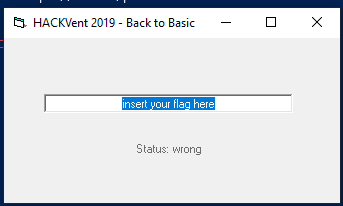
\includegraphics{./basic.png}
\caption{Screenshot}
\end{figure}

So the big question was how to get that into some readable format. At
the point I solved this challenge, I hadn't used Ghidra/IDA yet (I later
did on day 16). I also wasn't sure if it was the right tool for this
job, so I looked for VBA disassemblers.

I found \href{https://www.vb-decompiler.org/}{VB Decompiler} and
\href{https://qiil.io/}{VBReFormer} and used them to analyze the
function called when the entered text changed. Unfortunately, all the
free versions could produce was some 600 lines of disassembly.

At that point, I also found the string
\texttt{"6klzic\textless{}=bPBtdvff\textquotesingle{}y\textbackslash{}x7fFI\textasciitilde{}on//N"}
(not a literal \texttt{\textbackslash{}x7f}, but an ASCII DEL). This
will be important for alter

A big part of the disassembly looked like this:

\begin{verbatim}
loc_004020B5: mov esi, [00401054h] ; rtcMidCharVar
loc_004020BB: lea eax, var_5C
loc_004020BE: push eax
loc_004020BF: lea ecx, var_34
loc_004020C2: push 00000001h
loc_004020C4: lea edx, var_6C
loc_004020C7: mov ebx, 00000002h
loc_004020CC: push ecx
loc_004020CD: push edx
loc_004020CE: mov var_54, 00000001h
loc_004020D5: mov var_5C, ebx
loc_004020D8: call rtcMidCharVar
\end{verbatim}

In this snippet, the following happens:

\begin{itemize}
\tightlist
\item
  \texttt{var\_54} is set to 1
\item
  \texttt{var\_5C} is set to 2 (via \texttt{ebx} which was set earlier)
\item
  A call to the
  \href{https://docs.microsoft.com/en-us/office/vba/language/reference/user-interface-help/mid-function}{\texttt{Mid}
  Visual Basic function}
\end{itemize}

To understand how the VisualBasic calls worked, I mainly used a
\href{https://hvoidcode.wordpress.com/2016/02/06/vb-function-description-for-reversing/}{weirdly
formatted blogpost} and the
\href{https://blog.csdn.net/weixin_30736301/article/details/95964460}{Chinese
original}. Here's an example, based on the same code, but shortened and
rearranged:

\begin{verbatim}
lea eax, var_5C
push eax

push 00000001h

lea ecx, var_34
push ecx

lea edx, var_6C
push edx

call rtcMidCharVar
\end{verbatim}

The calling convention seems to be so that this corresponds to:

\begin{verbatim}
var_6C = Mid(var_34, 1, var_5C)
\end{verbatim}

I basically did that for some six hours until I had an idea what the
application was doing. Two things made this much more difficult:

\begin{itemize}
\tightlist
\item
  At some points where I was supposed to see some data, I only saw
  0x8008 (same when looking at the file in Ghidra as part of writing
  this writeup)
\item
  Some arguments in the disassembly seemed to be wrong. For example, for
  a (very important) \texttt{for}-loop which starts with 6,
  \texttt{var\_164} is set to 6 (and never used), but then
  \texttt{\_\_vbaVarForInit} is called with \texttt{var\_6C},
  \texttt{var\_16C}, \texttt{var\_1E4}, \texttt{var\_1D4} and
  \texttt{var\_24}. The VBReFormer tool ended up showing me
  \texttt{For\ var\_24\ =\ var\_25\ To\ \#NOT\ SUPPORTED\#\ Step\ 1} but
  not showing me \texttt{var\_25} and \texttt{var\_25} anywhere.
\end{itemize}

Because of all those issues, I needed a hint or two from someone who
already solved the challenge.

After an excruciating six hours, I had an idea of what was happening -
here is a rough Python reimplementation (trying to more or less keep the
original structure, so not using Python idioms):

    \begin{tcolorbox}[breakable, size=fbox, boxrule=1pt, pad at break*=1mm,colback=cellbackground, colframe=cellborder]
\prompt{In}{incolor}{19}{\boxspacing}
\begin{Verbatim}[commandchars=\\\{\}]
\PY{n}{DATA} \PY{o}{=} \PY{l+s+sa}{b}\PY{l+s+s2}{\PYZdq{}}\PY{l+s+s2}{6klzic\PYZlt{}=bPBtdvff}\PY{l+s+s2}{\PYZsq{}}\PY{l+s+s2}{y}\PY{l+s+se}{\PYZbs{}x7f}\PY{l+s+s2}{FI\PYZti{}on//N}\PY{l+s+s2}{\PYZdq{}}

\PY{k}{def} \PY{n+nf}{check}\PY{p}{(}\PY{n}{inp}\PY{p}{)}\PY{p}{:}
    \PY{n}{mid1} \PY{o}{=} \PY{n}{inp}\PY{p}{[}\PY{l+m+mi}{0}\PY{p}{]} \PY{c+c1}{\PYZsh{} 004020B5}
    \PY{n}{mid2} \PY{o}{=} \PY{n}{inp}\PY{p}{[}\PY{l+m+mi}{1}\PY{p}{]} \PY{c+c1}{\PYZsh{} 004020DA}
    \PY{n}{mid3} \PY{o}{=} \PY{n}{inp}\PY{p}{[}\PY{l+m+mi}{2}\PY{p}{]} \PY{c+c1}{\PYZsh{} 00402113}
    \PY{n}{mid4} \PY{o}{=} \PY{n}{inp}\PY{p}{[}\PY{l+m+mi}{3}\PY{p}{]} \PY{c+c1}{\PYZsh{} 0040214D}
    
    \PY{n}{ok} \PY{o}{=} \PY{n}{mid1} \PY{o}{==} \PY{l+s+s1}{\PYZsq{}}\PY{l+s+s1}{H}\PY{l+s+s1}{\PYZsq{}}  \PY{c+c1}{\PYZsh{} 00402187}
    
    \PY{n}{ok2} \PY{o}{=} \PY{n}{mid2} \PY{o}{==} \PY{l+s+s1}{\PYZsq{}}\PY{l+s+s1}{V}\PY{l+s+s1}{\PYZsq{}} \PY{c+c1}{\PYZsh{} 004021B0}
    \PY{n}{ok} \PY{o}{\PYZam{}}\PY{o}{=} \PY{n}{ok2}         \PY{c+c1}{\PYZsh{} 004021CC}
    
    \PY{n}{ok3} \PY{o}{=} \PY{n}{mid3} \PY{o}{==} \PY{l+s+s1}{\PYZsq{}}\PY{l+s+s1}{1}\PY{l+s+s1}{\PYZsq{}} \PY{c+c1}{\PYZsh{} 004021DA}
    \PY{n}{ok} \PY{o}{\PYZam{}}\PY{o}{=} \PY{n}{ok3}         \PY{c+c1}{\PYZsh{} 004021F6}
    
    \PY{n}{ok4} \PY{o}{=} \PY{n}{mid4} \PY{o}{==} \PY{l+s+s1}{\PYZsq{}}\PY{l+s+s1}{9}\PY{l+s+s1}{\PYZsq{}} \PY{c+c1}{\PYZsh{} 00402204}
    \PY{n}{ok} \PY{o}{\PYZam{}}\PY{o}{=} \PY{n}{ok4}         \PY{c+c1}{\PYZsh{} 00402220}
    
    \PY{k}{assert} \PY{n}{ok}
    
    \PY{n}{length} \PY{o}{=} \PY{n+nb}{len}\PY{p}{(}\PY{n}{inp}\PY{p}{)}    \PY{c+c1}{\PYZsh{} 00402286}
    \PY{k}{assert} \PY{n}{length} \PY{o}{==} \PY{l+m+mi}{33}  \PY{c+c1}{\PYZsh{} 004022A8}
    
    \PY{k}{for} \PY{n}{i} \PY{o+ow}{in} \PY{n+nb}{range}\PY{p}{(}\PY{l+m+mi}{6}\PY{p}{,} \PY{l+m+mi}{33}\PY{p}{)}\PY{p}{:}  \PY{c+c1}{\PYZsh{} 004022BF to 0040232D}
        \PY{k}{assert} \PY{n+nb}{ord}\PY{p}{(}\PY{n}{inp}\PY{p}{[}\PY{n}{i}\PY{o}{\PYZhy{}}\PY{l+m+mi}{1}\PY{p}{]}\PY{p}{)} \PY{o}{\PYZca{}} \PY{n}{i} \PY{o}{==} \PY{n}{DATA}\PY{p}{[}\PY{n}{i}\PY{o}{\PYZhy{}}\PY{l+m+mi}{6}\PY{p}{]}  \PY{c+c1}{\PYZsh{} 00402339 to 004023C0}
\end{Verbatim}
\end{tcolorbox}

    So we can get the flag based on that weird string we found initially:

    \begin{tcolorbox}[breakable, size=fbox, boxrule=1pt, pad at break*=1mm,colback=cellbackground, colframe=cellborder]
\prompt{In}{incolor}{20}{\boxspacing}
\begin{Verbatim}[commandchars=\\\{\}]
\PY{n+nb}{print}\PY{p}{(}\PY{l+s+s1}{\PYZsq{}}\PY{l+s+s1}{HV19}\PY{l+s+s1}{\PYZob{}}\PY{l+s+s1}{\PYZsq{}} \PY{o}{+} \PY{l+s+s1}{\PYZsq{}}\PY{l+s+s1}{\PYZsq{}}\PY{o}{.}\PY{n}{join}\PY{p}{(}\PY{n+nb}{chr}\PY{p}{(}\PY{n}{k} \PY{o}{\PYZca{}} \PY{n}{i}\PY{p}{)} \PY{k}{for} \PY{n}{i}\PY{p}{,} \PY{n}{k} \PY{o+ow}{in} \PY{n+nb}{enumerate}\PY{p}{(}\PY{n}{DATA}\PY{p}{,} \PY{n}{start}\PY{o}{=}\PY{l+m+mi}{6}\PY{p}{)}\PY{p}{)} \PY{o}{+} \PY{l+s+s1}{\PYZsq{}}\PY{l+s+s1}{\PYZcb{}}\PY{l+s+s1}{\PYZsq{}}\PY{p}{)}
\end{Verbatim}
\end{tcolorbox}

    \begin{Verbatim}[commandchars=\\\{\}]
HV19\{0ldsch00l\_Revers1ng\_Sess10n\}
    \end{Verbatim}



    
\pagebreak{}
    \hypertarget{hv19.13-trieme}{%
\section{HV19.13 TrieMe}\label{hv19.13-trieme}}

\begin{quote}
Switzerland's national security is at risk. As you try to infiltrate a
secret spy facility to save the nation you stumble upon an interesting
looking login portal.

Can you break it and retrieve the critical information?
\end{quote}

We get a website and some code - here's the part I consider important:

\begin{Shaded}
\begin{Highlighting}[]
\KeywordTok{import}\ImportTok{ org.apache.commons.collections4.trie.PatriciaTrie;}
\KeywordTok{import static}\ImportTok{ org.apache.commons.lang3.StringEscapeUtils.unescapeJava;}

\KeywordTok{public} \KeywordTok{class}\NormalTok{ NotesBean }\KeywordTok{implements} \BuiltInTok{Serializable}\NormalTok{ \{}
    \KeywordTok{private}\NormalTok{ PatriciaTrie<}\BuiltInTok{Integer}\NormalTok{> trie = }\FunctionTok{init}\NormalTok{();}
    \KeywordTok{private} \DataTypeTok{static} \DataTypeTok{final} \BuiltInTok{String}\NormalTok{ securitytoken = }\StringTok{"auth\_token\_4835989"}\NormalTok{;}

    \KeywordTok{public} \FunctionTok{NotesBean}\NormalTok{() \{}
        \KeywordTok{super}\NormalTok{();}
        \FunctionTok{init}\NormalTok{();}
\NormalTok{    \}}

    \KeywordTok{public} \BuiltInTok{String} \FunctionTok{getTrie}\NormalTok{() }\KeywordTok{throws} \BuiltInTok{IOException}\NormalTok{ \{}
        \KeywordTok{if}\NormalTok{(}\FunctionTok{isAdmin}\NormalTok{(trie)) \{ }\CommentTok{/* show flag */}\NormalTok{ \}}
        \KeywordTok{return} \StringTok{"INTRUSION WILL BE REPORTED!"}\NormalTok{;}
\NormalTok{    \}}

    \KeywordTok{public} \DataTypeTok{void} \FunctionTok{setTrie}\NormalTok{(}\BuiltInTok{String}\NormalTok{ note) \{}
\NormalTok{        trie.}\FunctionTok{put}\NormalTok{(}\FunctionTok{unescapeJava}\NormalTok{(note), }\DecValTok{0}\NormalTok{);}
\NormalTok{    \}}
        
    \KeywordTok{private} \DataTypeTok{static}\NormalTok{ PatriciaTrie<}\BuiltInTok{Integer}\NormalTok{> }\FunctionTok{init}\NormalTok{()\{}
\NormalTok{        PatriciaTrie<}\BuiltInTok{Integer}\NormalTok{> trie = }\KeywordTok{new}\NormalTok{ PatriciaTrie<}\BuiltInTok{Integer}\NormalTok{>();}
\NormalTok{        trie.}\FunctionTok{put}\NormalTok{(securitytoken,}\DecValTok{0}\NormalTok{);}
        \KeywordTok{return}\NormalTok{ trie;}
\NormalTok{    \}}

    \KeywordTok{private} \DataTypeTok{static} \DataTypeTok{boolean} \FunctionTok{isAdmin}\NormalTok{(PatriciaTrie<}\BuiltInTok{Integer}\NormalTok{> trie)\{}
        \KeywordTok{return}\NormalTok{ !trie.}\FunctionTok{containsKey}\NormalTok{(securitytoken);}
\NormalTok{    \}}
\NormalTok{\}}
\end{Highlighting}
\end{Shaded}

I can see two ways of getting the flag:

\begin{itemize}
\tightlist
\item
  Reading the file somehow
\item
  Somehow finding a way to make the trie not contain the securitytoken
  anymore
\end{itemize}

We have:

\begin{itemize}
\tightlist
\item
  A
  \href{https://commons.apache.org/proper/commons-collections/apidocs/org/apache/commons/collections4/trie/PatriciaTrie.html}{PatriciaTree}
\item
  A
  \href{https://commons.apache.org/proper/commons-lang/apidocs/org/apache/commons/lang3/StringEscapeUtils.html\#unescapeJava-java.lang.String-}{unescapeJava}
  call (deprecated, but only moved to
  \href{http://commons.apache.org/proper/commons-text/javadocs/api-release/index.html}{commons.text})
\end{itemize}

After some Googling for \texttt{PatriciaTrie} and \texttt{containsKey} I
found an article,
\href{https://www.pentagrid.ch/de/blog/fuzzing_java_with_jqf/}{Fuzzing
Java with JQF}. It's written by
\href{https://www.pentagrid.ch/}{Pentagrid} (a Swiss security company),
and \href{https://twitter.com/xorkiwi}{xorkiwi} (the author) is from
Switzerland as well (maybe even working there?). Seems like a great
starting point!

The article talks about fuzzing \texttt{PatriciaKey.containsKey}, where
did something like:

\begin{Shaded}
\begin{Highlighting}[]
\CommentTok{// [...]}
\FunctionTok{assumeTrue}\NormalTok{(map.}\FunctionTok{containsKey}\NormalTok{(key));}
\NormalTok{PatriciaTrie trie = }\KeywordTok{new} \FunctionTok{PatriciaTrie}\NormalTok{(map);}
\FunctionTok{assertTrue}\NormalTok{(trie.}\FunctionTok{containsKey}\NormalTok{(key));}
\end{Highlighting}
\end{Shaded}

and found that this doesn't hold true for a key with a null-byte:

\begin{verbatim}
Key in UTF-16 hexadecimal: 0000
[...]
java.lang.AssertionError
\end{verbatim}

Thanks to the \texttt{unescapeJava} call, we can use an input like
\texttt{\textbackslash{}u0000} to insert a null byte into the trie. That
didn't work, but I was pretty sure I was on the right track, everything
just fit together nicely.

Given that we want to get \texttt{auth\_token\_4835989} ``out'' of the
tree, I tried \texttt{auth\_token\_4835989\textbackslash{}u0000} which
worked and presented me with the flag:

\begin{quote}
STATUS: We will steal all the national chocolate supplies at christmas,
3pm: Here's the building codes: HV19\{get\_th3\_chocolateZ\} !
\end{quote}

After solving the challenge, I also found the corresponding bug report
where this issue is discussed in more detail:
\href{https://issues.apache.org/jira/browse/COLLECTIONS-714}{PatriciaTrie
ignores trailing null characters in keys}.


    
\pagebreak{}
    \hypertarget{hv19.14-achtung-das-flag}{%
\section{HV19.14 Achtung das Flag}\label{hv19.14-achtung-das-flag}}

\emph{Let's play another little game this year. Once again, I promise it
is hardly obfuscated.}

For this challenge, we get the following Perl \sout{garbage} script:

\begin{Shaded}
\begin{Highlighting}[]
\FunctionTok{use}\NormalTok{ Tk;}\FunctionTok{use} \FunctionTok{MIME::Base64}\NormalTok{;}\FunctionTok{chomp}\NormalTok{((}\DataTypeTok{$a}\NormalTok{,}\DataTypeTok{$a}\NormalTok{,}\DataTypeTok{$b}\NormalTok{,}\DataTypeTok{$c}\NormalTok{,}\DataTypeTok{$f}\NormalTok{,}\DataTypeTok{$u}\NormalTok{,}\DataTypeTok{$z}\NormalTok{,}\DataTypeTok{$y}\NormalTok{,}\DataTypeTok{$r}\NormalTok{,}\DataTypeTok{$r}\NormalTok{,}\DataTypeTok{$u}\NormalTok{)=}\KeywordTok{<DATA>}\NormalTok{);}\KeywordTok{sub }\FunctionTok{M}\NormalTok{\{}\DataTypeTok{$M}\NormalTok{=}\FunctionTok{shift}\NormalTok{;}\CommentTok{\#\#}
\DataTypeTok{@m}\NormalTok{=}\FunctionTok{keys}\NormalTok{ \%::;(}\FunctionTok{grep}\NormalTok{\{(}\FunctionTok{unpack}\NormalTok{(}\KeywordTok{"}\DataTypeTok{\%32W}\StringTok{*}\KeywordTok{"}\NormalTok{,}\DataTypeTok{$\_}\NormalTok{).}\FunctionTok{length}\NormalTok{(}\DataTypeTok{$\_}\NormalTok{))eq}\DataTypeTok{$M}\NormalTok{\}}\DataTypeTok{@m}\NormalTok{)[}\DecValTok{0}\NormalTok{]\};}\DataTypeTok{$zvYPxUpXMSsw}\NormalTok{=}\BaseNTok{0x1337C0DE}\NormalTok{;}\CommentTok{\#\#\#}
\KeywordTok{/}\OtherTok{\_help\_me\_}\KeywordTok{/}\NormalTok{;}\DataTypeTok{$PMMtQJOcHm8eFQfdsdNAS20}\NormalTok{=}\KeywordTok{sub}\NormalTok{\{}\DataTypeTok{$zvYPxUpXMSsw}\NormalTok{=(}\DataTypeTok{$zvYPxUpXMSsw}\NormalTok{*}\DecValTok{16807}\NormalTok{)\&}\BaseNTok{0xFFFFFFFF}\NormalTok{;\};}
\NormalTok{(}\DataTypeTok{$a1Ivn0ECw49I5I0oE0}\NormalTok{=}\KeywordTok{\textquotesingle{}}\StringTok{07\&3{-}"11*/(}\KeywordTok{\textquotesingle{}}\NormalTok{)=\textasciitilde{}}\KeywordTok{y}\OtherTok{$!{-}=$\textasciigrave{}{-}\textasciitilde{}$;($Sk61A7pO=\textquotesingle{}K\&:P3\&44\textquotesingle{})=\textasciitilde{}y$!{-}=$\textasciigrave{}{-}\textasciitilde{}$}\NormalTok{;}\KeywordTok{m/}\OtherTok{Mm}\KeywordTok{/g}\NormalTok{;}
\NormalTok{(}\DataTypeTok{$sk6i47pO}\NormalTok{=}\KeywordTok{\textquotesingle{}}\StringTok{K\&:R\&{-}\&"4\&}\KeywordTok{\textquotesingle{}}\NormalTok{)=\textasciitilde{}}\KeywordTok{y}\OtherTok{$!{-}=$\textasciigrave{}{-}\textasciitilde{}$;;;;$d28Vt03MEbdY0=sub\{pack(\textquotesingle{}n\textquotesingle{},$fff[$}\NormalTok{S9cXJIGB0BWce++]}
\NormalTok{\^{}(}\DataTypeTok{$PMMtQJOcHm8eFQfdsdNAS20}\NormalTok{{-}>()\&}\BaseNTok{0xDEAD}\NormalTok{));\};}\KeywordTok{\textquotesingle{}}\StringTok{42}\KeywordTok{\textquotesingle{}}\NormalTok{;(}\DataTypeTok{$vgOjwRk4wIo7\_}\NormalTok{=MainWindow{-}>new){-}>title(}\DataTypeTok{$r}\NormalTok{)}
\NormalTok{;(}\DataTypeTok{$vMnyQdAkfgIIik}\NormalTok{=}\DataTypeTok{$vgOjwRk4wIo7\_}\NormalTok{{-}>}\DataTypeTok{Canvas}\NormalTok{(}\KeywordTok{"}\StringTok{{-}}\DataTypeTok{$a}\KeywordTok{"}\NormalTok{=>}\DecValTok{640}\NormalTok{,}\KeywordTok{"}\StringTok{{-}}\DataTypeTok{$b}\KeywordTok{"}\NormalTok{=>}\DecValTok{480}\NormalTok{,}\KeywordTok{"}\StringTok{{-}}\DataTypeTok{$u}\KeywordTok{"}\NormalTok{=>}\DataTypeTok{$f}\NormalTok{)){-}>}\FunctionTok{pack}\NormalTok{;}\DataTypeTok{@p}\NormalTok{=(}\DecValTok{42}\NormalTok{,}\DecValTok{42}
\NormalTok{);}\DataTypeTok{$cqI}\NormalTok{=}\DataTypeTok{$vMnyQdAkfgIIik}\NormalTok{{-}>}\DataTypeTok{createLine}\NormalTok{(}\DataTypeTok{@p}\NormalTok{,}\DataTypeTok{@p}\NormalTok{,}\KeywordTok{"}\StringTok{{-}}\DataTypeTok{$y}\KeywordTok{"}\NormalTok{=>}\DataTypeTok{$c}\NormalTok{,}\KeywordTok{"}\StringTok{{-}}\DataTypeTok{$a}\KeywordTok{"}\NormalTok{=>}\DecValTok{3}\NormalTok{);;;}\DataTypeTok{$S9cXJIGB0BWce}\NormalTok{=}\DecValTok{0}\NormalTok{;}\DataTypeTok{$\_2kY10}\NormalTok{=}\DecValTok{0}\NormalTok{;}
\DataTypeTok{$\_8NZQooI5K4b}\NormalTok{=}\DecValTok{0}\NormalTok{;}\DataTypeTok{$Sk6lA7p0}\NormalTok{=}\DecValTok{0}\NormalTok{;}\DataTypeTok{$MMM\_\_}\NormalTok{;}\DataTypeTok{$\_}\NormalTok{=M(}\DecValTok{120812}\NormalTok{).}\KeywordTok{\textquotesingle{}}\StringTok{/}\KeywordTok{\textquotesingle{}}\NormalTok{.M(}\DecValTok{191323}\NormalTok{).M(}\DecValTok{133418}\NormalTok{).M(}\DecValTok{98813}\NormalTok{).M(}\DecValTok{121913}\NormalTok{)}
\NormalTok{.M(}\DecValTok{134214}\NormalTok{).M(}\DecValTok{101213}\NormalTok{).}\KeywordTok{\textquotesingle{}}\StringTok{/}\KeywordTok{\textquotesingle{}}\NormalTok{.M(}\DecValTok{97312}\NormalTok{).M(}\DecValTok{6328}\NormalTok{).M(}\DecValTok{2853}\NormalTok{).}\KeywordTok{\textquotesingle{}}\StringTok{+}\KeywordTok{\textquotesingle{}}\NormalTok{.M(}\DecValTok{4386}\NormalTok{);}\KeywordTok{s|}\OtherTok{\_}\CharTok{||}\OtherTok{gi;}\DataTypeTok{@fff}\OtherTok{=map\{unpack}\CharTok{(}\OtherTok{\textquotesingle{}n\textquotesingle{},}
\CharTok{$}\OtherTok{::\{M}\CharTok{(}\OtherTok{122413}\CharTok{)}\OtherTok{\}{-}>}\CharTok{($}\OtherTok{\_}\CharTok{))}\OtherTok{\}m:...:g;}\CharTok{($}\OtherTok{T=sub\{}\CharTok{$}\OtherTok{vMnyQdAkfgIIik{-}>delete}\CharTok{($}\OtherTok{t}\CharTok{)}\OtherTok{;}\CharTok{$}\OtherTok{t=}\CharTok{$}\OtherTok{vMnyQdAkfgIIik{-}>\#FOO}
\OtherTok{createText}\CharTok{($}\OtherTok{PMMtQJOcHm8eFQfdsdNAS20{-}>}\CharTok{()}\OtherTok{\%600}\CharTok{+}\OtherTok{20,}\CharTok{$}\OtherTok{PMMtQJOcHm8eFQfdsdNAS20{-}>}\CharTok{()}\OtherTok{\%440}\CharTok{+}\OtherTok{20,\#Perl!!}
\OtherTok{"{-}text"=>}\CharTok{$}\OtherTok{d28Vt03MEbdY0{-}>}\CharTok{()}\OtherTok{,"{-}}\CharTok{$}\OtherTok{y"=>}\CharTok{$}\OtherTok{z}\CharTok{)}\OtherTok{;\}}\CharTok{)}\OtherTok{{-}>}\CharTok{()}\OtherTok{;}\CharTok{$}\OtherTok{HACK;}\CharTok{$}\OtherTok{i=}\CharTok{$}\OtherTok{vMnyQdAkfgIIik{-}>repeat}\CharTok{(}\OtherTok{25,sub\{}\CharTok{$}\OtherTok{\_=}\CharTok{(}
\CharTok{$}\OtherTok{\_8NZQooI5K4b}\CharTok{+}\OtherTok{=0.1}\CharTok{*$}\OtherTok{Sk6lA7p0}\CharTok{)}\OtherTok{;;}\CharTok{$}\OtherTok{p}\CharTok{[}\BaseNTok{0}\CharTok{]+}\OtherTok{=3.0}\CharTok{*}\OtherTok{cos;}\CharTok{$}\OtherTok{p}\CharTok{[}\BaseNTok{1}\CharTok{]}\OtherTok{{-}=3}\CharTok{*}\OtherTok{sin;;}\CharTok{($}\OtherTok{p}\CharTok{[}\BaseNTok{0}\CharTok{]}\OtherTok{>1\&\&}\CharTok{$}\OtherTok{p}\CharTok{[}\BaseNTok{1}\CharTok{]}\OtherTok{>1\&\&}\CharTok{$}\OtherTok{p}\CharTok{[}\BaseNTok{0}\CharTok{]}\OtherTok{<639\&\&}
\CharTok{$}\OtherTok{p}\CharTok{[}\BaseNTok{1}\CharTok{]}\OtherTok{<479}\CharTok{)||$}\OtherTok{i{-}>cancel}\CharTok{()}\OtherTok{;00;}\CharTok{$}\OtherTok{q=}\CharTok{($}\OtherTok{vMnyQdAkfgIIik{-}>find}\CharTok{($}\OtherTok{a1Ivn0ECw49I5I0oE0,}\CharTok{$}\OtherTok{p}\CharTok{[}\BaseNTok{0}\CharTok{]}\OtherTok{{-}1,}\CharTok{$}\OtherTok{p}\CharTok{[}\BaseNTok{1}\CharTok{]}\OtherTok{{-}1,}
\CharTok{$}\OtherTok{p}\CharTok{[}\BaseNTok{0}\CharTok{]+}\OtherTok{1,}\CharTok{$}\OtherTok{p}\CharTok{[}\BaseNTok{1}\CharTok{]+}\OtherTok{1}\CharTok{)||[])}\OtherTok{{-}>}\CharTok{[}\BaseNTok{0}\CharTok{]}\OtherTok{;}\CharTok{$}\OtherTok{q==}\CharTok{$}\OtherTok{t\&\&}\CharTok{$}\OtherTok{T{-}>}\CharTok{()}\OtherTok{;}\CharTok{$}\OtherTok{vMnyQdAkfgIIik{-}>insert}\CharTok{($}\OtherTok{cqI,\textquotesingle{}end\textquotesingle{},\textbackslash{}@p}\CharTok{)}\OtherTok{;}\CharTok{($}\OtherTok{q==\#\#\#}
\CharTok{$}\OtherTok{cqI}\CharTok{||$}\OtherTok{S9cXJIGB0BWce>44}\CharTok{)}\OtherTok{\&\&}\CharTok{$}\OtherTok{i{-}>cancel}\CharTok{()}\OtherTok{;\}}\CharTok{)}\OtherTok{;}\CharTok{$}\OtherTok{KE=5;}\CharTok{$}\OtherTok{vgOjwRk4wIo7\_{-}>bind}\CharTok{(}\OtherTok{"<}\CharTok{$}\OtherTok{Sk61A7pO{-}n>"=>sub\{}
\CharTok{$}\OtherTok{Sk6lA7p0=1;\}}\CharTok{)}\OtherTok{;}\CharTok{$}\OtherTok{vgOjwRk4wIo7\_{-}>bind}\CharTok{(}\OtherTok{"<}\CharTok{$}\OtherTok{Sk61A7pO{-}m>"=>sub\{}\CharTok{$}\OtherTok{Sk6lA7p0={-}1;\}}\CharTok{)}\OtherTok{;}\CharTok{$}\OtherTok{vgOjwRk4wIo7\_\#\%"}
\OtherTok{{-}>bind}\CharTok{(}\OtherTok{"<}\CharTok{$}\OtherTok{sk6i47pO{-}n>"=>sub\{}\CharTok{$}\OtherTok{Sk6lA7p0=0 if}\CharTok{$}\OtherTok{Sk6lA7p0>0;\}}\CharTok{)}\OtherTok{;}\CharTok{$}\OtherTok{vgOjwRk4wIo7\_{-}>bind}\CharTok{(}\OtherTok{"<}\CharTok{$}\OtherTok{sk6i47pO"}
\OtherTok{."{-}m>"=>sub\{}\CharTok{$}\OtherTok{Sk6lA7p0=0 if }\CharTok{$}\OtherTok{Sk6lA7p0<0;\}}\CharTok{)}\OtherTok{;}\CharTok{$}\OtherTok{::\{M}\CharTok{(}\OtherTok{7998}\CharTok{)}\OtherTok{\}{-}>}\CharTok{()}\OtherTok{;}\CharTok{$}\OtherTok{M\_decrypt=sub\{\textquotesingle{}HACKVENT2019\textquotesingle{}\};}
\OtherTok{\_\_DATA\_\_}
\OtherTok{The cake is a lie!}
\OtherTok{width}
\OtherTok{height}
\OtherTok{orange}
\OtherTok{black}
\OtherTok{green}
\OtherTok{cyan}
\OtherTok{fill}
\OtherTok{Only perl can parse Perl!}
\OtherTok{Achtung das Flag! {-}{-}> Use N and M}
\OtherTok{background}
\OtherTok{M\textquotesingle{}}\CharTok{)}\OtherTok{; DROP TABLE flags; {-}{-} }
\OtherTok{Run me in Perl!}
\OtherTok{\_\_DATA\_\_}
\end{Highlighting}
\end{Shaded}

When running the script, something quite surprising happens: We get a
Snake-like game inspired by \href{https://achtungdiekurve.net/}{Achtung,
die Kurve!} which allows us to get the flag by eating parts of it:

\begin{figure}
\centering
\includegraphics{./snake.png}
\caption{Snake screenshot}
\end{figure}

I got as far as \texttt{HV19\{s@@jSfx}, but at some point, the game is
much too hard to play.

I started by adding some newlines to the source:

\begin{Shaded}
\begin{Highlighting}[]
\FunctionTok{use}\NormalTok{ Tk;}
\FunctionTok{use} \FunctionTok{MIME::Base64}\NormalTok{;}

\FunctionTok{chomp}\NormalTok{((}\DataTypeTok{$a}\NormalTok{,}\DataTypeTok{$a}\NormalTok{,}\DataTypeTok{$b}\NormalTok{,}\DataTypeTok{$c}\NormalTok{,}\DataTypeTok{$f}\NormalTok{,}\DataTypeTok{$u}\NormalTok{,}\DataTypeTok{$z}\NormalTok{,}\DataTypeTok{$y}\NormalTok{,}\DataTypeTok{$r}\NormalTok{,}\DataTypeTok{$r}\NormalTok{,}\DataTypeTok{$u}\NormalTok{)=}\KeywordTok{<DATA>}\NormalTok{);}

\KeywordTok{sub }\FunctionTok{M}\NormalTok{\{}
    \DataTypeTok{$M}\NormalTok{=}\FunctionTok{shift}\NormalTok{;}
    \DataTypeTok{@m}\NormalTok{=}\FunctionTok{keys}\NormalTok{ \%::;}
    \DataTypeTok{$F}\NormalTok{ = (}\FunctionTok{grep}\NormalTok{\{(}\FunctionTok{unpack}\NormalTok{(}\KeywordTok{"}\DataTypeTok{\%32W}\StringTok{*}\KeywordTok{"}\NormalTok{,}\DataTypeTok{$\_}\NormalTok{).}\FunctionTok{length}\NormalTok{(}\DataTypeTok{$\_}\NormalTok{))eq}\DataTypeTok{$M}\NormalTok{\}}\DataTypeTok{@m}\NormalTok{)[}\DecValTok{0}\NormalTok{];}
    \DataTypeTok{$F}\NormalTok{;}
\NormalTok{\};}

\DataTypeTok{$zvYPxUpXMSsw}\NormalTok{=}\BaseNTok{0x1337C0DE}\NormalTok{;}
\DataTypeTok{$PMMtQJOcHm8eFQfdsdNAS20}\NormalTok{=}\KeywordTok{sub}\NormalTok{\{}\DataTypeTok{$zvYPxUpXMSsw}\NormalTok{=(}\DataTypeTok{$zvYPxUpXMSsw}\NormalTok{*}\DecValTok{16807}\NormalTok{)\&}\BaseNTok{0xFFFFFFFF}\NormalTok{;\};}

\NormalTok{(}\DataTypeTok{$a1Ivn0ECw49I5I0oE0}\NormalTok{=}\KeywordTok{\textquotesingle{}}\StringTok{07\&3{-}"11*/(}\KeywordTok{\textquotesingle{}}\NormalTok{)=\textasciitilde{}}\KeywordTok{y}\OtherTok{$!{-}=$\textasciigrave{}{-}\textasciitilde{}$}\NormalTok{;}
\NormalTok{(}\DataTypeTok{$Sk61A7pO}\NormalTok{=}\KeywordTok{\textquotesingle{}}\StringTok{K\&:P3\&44}\KeywordTok{\textquotesingle{}}\NormalTok{)=\textasciitilde{}}\KeywordTok{y}\OtherTok{$!{-}=$\textasciigrave{}{-}\textasciitilde{}$}\NormalTok{;}

\NormalTok{(}\DataTypeTok{$sk6i47pO}\NormalTok{=}\KeywordTok{\textquotesingle{}}\StringTok{K\&:R\&{-}\&"4\&}\KeywordTok{\textquotesingle{}}\NormalTok{)=\textasciitilde{}}\KeywordTok{y}\OtherTok{$!{-}=$\textasciigrave{}{-}\textasciitilde{}$}\NormalTok{;}

\DataTypeTok{$d28Vt03MEbdY0}\NormalTok{=}\KeywordTok{sub}\NormalTok{\{}
    \DataTypeTok{$res}\NormalTok{ = }\FunctionTok{pack}\NormalTok{(}\KeywordTok{\textquotesingle{}}\StringTok{n}\KeywordTok{\textquotesingle{}}\NormalTok{,}\DataTypeTok{$fff}\NormalTok{[}\DataTypeTok{$S9cXJIGB0BWce}\NormalTok{++]\^{}(}\DataTypeTok{$PMMtQJOcHm8eFQfdsdNAS20}\NormalTok{{-}>()\&}\BaseNTok{0xDEAD}\NormalTok{));}
    \FunctionTok{print} \KeywordTok{"}\DataTypeTok{$res}\KeywordTok{"}\NormalTok{;}
    \DataTypeTok{$res}\NormalTok{;}
\NormalTok{\};}

\NormalTok{(}\DataTypeTok{$vgOjwRk4wIo7\_}\NormalTok{=MainWindow{-}>new){-}>title(}\DataTypeTok{$r}\NormalTok{);}
\NormalTok{(}\DataTypeTok{$vMnyQdAkfgIIik}\NormalTok{=}\DataTypeTok{$vgOjwRk4wIo7\_}\NormalTok{{-}>}\DataTypeTok{Canvas}\NormalTok{(}\KeywordTok{"}\StringTok{{-}}\DataTypeTok{$a}\KeywordTok{"}\NormalTok{=>}\DecValTok{640}\NormalTok{,}\KeywordTok{"}\StringTok{{-}}\DataTypeTok{$b}\KeywordTok{"}\NormalTok{=>}\DecValTok{480}\NormalTok{,}\KeywordTok{"}\StringTok{{-}}\DataTypeTok{$u}\KeywordTok{"}\NormalTok{=>}\DataTypeTok{$f}\NormalTok{)){-}>}\FunctionTok{pack}\NormalTok{;}
\DataTypeTok{@p}\NormalTok{=(}\DecValTok{42}\NormalTok{,}\DecValTok{42}\NormalTok{);}
\DataTypeTok{$cqI}\NormalTok{=}\DataTypeTok{$vMnyQdAkfgIIik}\NormalTok{{-}>}\DataTypeTok{createLine}\NormalTok{(}\DataTypeTok{@p}\NormalTok{,}\DataTypeTok{@p}\NormalTok{,}\KeywordTok{"}\StringTok{{-}}\DataTypeTok{$y}\KeywordTok{"}\NormalTok{=>}\DataTypeTok{$c}\NormalTok{,}\KeywordTok{"}\StringTok{{-}}\DataTypeTok{$a}\KeywordTok{"}\NormalTok{=>}\DecValTok{3}\NormalTok{);}
\DataTypeTok{$S9cXJIGB0BWce}\NormalTok{=}\DecValTok{0}\NormalTok{;}
\DataTypeTok{$\_2kY10}\NormalTok{=}\DecValTok{0}\NormalTok{;}
\DataTypeTok{$\_8NZQooI5K4b}\NormalTok{=}\DecValTok{0}\NormalTok{;}
\DataTypeTok{$Sk6lA7p0}\NormalTok{=}\DecValTok{0}\NormalTok{;}
\DataTypeTok{$\_}\NormalTok{=M(}\DecValTok{120812}\NormalTok{).}\KeywordTok{\textquotesingle{}}\StringTok{/}\KeywordTok{\textquotesingle{}}\NormalTok{.M(}\DecValTok{191323}\NormalTok{).M(}\DecValTok{133418}\NormalTok{).M(}\DecValTok{98813}\NormalTok{).M(}\DecValTok{121913}\NormalTok{).M(}\DecValTok{134214}\NormalTok{).M(}\DecValTok{101213}\NormalTok{).}\KeywordTok{\textquotesingle{}}\StringTok{/}\KeywordTok{\textquotesingle{}}\NormalTok{.M(}\DecValTok{97312}\NormalTok{).M(}\DecValTok{6328}\NormalTok{).M(}\DecValTok{2853}\NormalTok{).}\KeywordTok{\textquotesingle{}}\StringTok{+}\KeywordTok{\textquotesingle{}}\NormalTok{.M(}\DecValTok{4386}\NormalTok{);}
\KeywordTok{s|}\OtherTok{\_}\CharTok{||}\OtherTok{gi;}

\DataTypeTok{@fff}\OtherTok{=map\{unpack}\CharTok{(}\OtherTok{\textquotesingle{}n\textquotesingle{}, }\CharTok{$}\OtherTok{::\{M}\CharTok{(}\OtherTok{122413}\CharTok{)}\OtherTok{\}{-}>}\CharTok{($}\OtherTok{\_}\CharTok{))}\OtherTok{\}m:...:g;}

\CharTok{($}\OtherTok{T=sub\{}
\OtherTok{     }\CharTok{$}\OtherTok{vMnyQdAkfgIIik{-}>delete}\CharTok{($}\OtherTok{t}\CharTok{)}\OtherTok{;}
\OtherTok{     }\CharTok{$}\OtherTok{t=}\CharTok{$}\OtherTok{vMnyQdAkfgIIik{-}>createText}\CharTok{($}\OtherTok{PMMtQJOcHm8eFQfdsdNAS20{-}>}\CharTok{()}\OtherTok{\%600}\CharTok{+}\OtherTok{20,}\CharTok{$}\OtherTok{PMMtQJOcHm8eFQfdsdNAS20{-}>}\CharTok{()}\OtherTok{\%440}\CharTok{+}\OtherTok{20,"{-}text"=>}\CharTok{$}\OtherTok{d28Vt03MEbdY0{-}>}\CharTok{()}\OtherTok{,"{-}}\CharTok{$}\OtherTok{y"=>}\CharTok{$}\OtherTok{z}\CharTok{)}\OtherTok{;}
\OtherTok{ \}}\CharTok{)}\OtherTok{{-}>}\CharTok{()}\OtherTok{;}
\OtherTok{ }
\CharTok{$}\OtherTok{i=}\CharTok{$}\OtherTok{vMnyQdAkfgIIik{-}>repeat}\CharTok{(}\OtherTok{25,}
\OtherTok{  sub\{}
\OtherTok{      }\CharTok{$}\OtherTok{\_=}\CharTok{($}\OtherTok{\_8NZQooI5K4b}\CharTok{+}\OtherTok{=0.1}\CharTok{*$}\OtherTok{Sk6lA7p0}\CharTok{)}\OtherTok{;}
\OtherTok{      ;}\CharTok{$}\OtherTok{p}\CharTok{[}\BaseNTok{0}\CharTok{]+}\OtherTok{=3.0}\CharTok{*}\OtherTok{cos;}\CharTok{$}\OtherTok{p}\CharTok{[}\BaseNTok{1}\CharTok{]}\OtherTok{{-}=3}\CharTok{*}\OtherTok{sin;;}\CharTok{($}\OtherTok{p}\CharTok{[}\BaseNTok{0}\CharTok{]}\OtherTok{>1\&\&}\CharTok{$}\OtherTok{p}\CharTok{[}\BaseNTok{1}\CharTok{]}\OtherTok{>1\&\&}\CharTok{$}\OtherTok{p}\CharTok{[}\BaseNTok{0}\CharTok{]}\OtherTok{<639\&\&}\CharTok{$}\OtherTok{p}\CharTok{[}\BaseNTok{1}\CharTok{]}\OtherTok{<479}\CharTok{)||$}\OtherTok{i{-}>cancel}\CharTok{()}\OtherTok{;}
\OtherTok{      00;}
\OtherTok{      }\CharTok{$}\OtherTok{q=}\CharTok{($}\OtherTok{vMnyQdAkfgIIik{-}>find}\CharTok{($}\OtherTok{a1Ivn0ECw49I5I0oE0,}\CharTok{$}\OtherTok{p}\CharTok{[}\BaseNTok{0}\CharTok{]}\OtherTok{{-}1,}\CharTok{$}\OtherTok{p}\CharTok{[}\BaseNTok{1}\CharTok{]}\OtherTok{{-}1, }\CharTok{$}\OtherTok{p}\CharTok{[}\BaseNTok{0}\CharTok{]+}\OtherTok{1,}\CharTok{$}\OtherTok{p}\CharTok{[}\BaseNTok{1}\CharTok{]+}\OtherTok{1}\CharTok{)||[])}\OtherTok{{-}>}\CharTok{[}\BaseNTok{0}\CharTok{]}\OtherTok{;}
\OtherTok{      }\CharTok{$}\OtherTok{q==}\CharTok{$}\OtherTok{t\&\&}\CharTok{$}\OtherTok{T{-}>}\CharTok{()}\OtherTok{;}
\OtherTok{      }\CharTok{$}\OtherTok{vMnyQdAkfgIIik{-}>insert}\CharTok{($}\OtherTok{cqI,\textquotesingle{}end\textquotesingle{},\textbackslash{}@p}\CharTok{)}\OtherTok{;}
\OtherTok{      }\CharTok{($}\OtherTok{q==}\CharTok{$}\OtherTok{cqI}\CharTok{||$}\OtherTok{S9cXJIGB0BWce>44}\CharTok{)}\OtherTok{\&\&}\CharTok{$}\OtherTok{i{-}>cancel}\CharTok{()}\OtherTok{;}
\OtherTok{  \}}\CharTok{)}\OtherTok{;}
\OtherTok{  }
\CharTok{$}\OtherTok{vgOjwRk4wIo7\_{-}>bind}\CharTok{(}\OtherTok{"<}\CharTok{$}\OtherTok{Sk61A7pO{-}n>"=>sub\{}\CharTok{$}\OtherTok{Sk6lA7p0=1;\}}\CharTok{)}\OtherTok{;}
\CharTok{$}\OtherTok{vgOjwRk4wIo7\_{-}>bind}\CharTok{(}\OtherTok{"<}\CharTok{$}\OtherTok{Sk61A7pO{-}m>"=>sub\{}\CharTok{$}\OtherTok{Sk6lA7p0={-}1;\}}\CharTok{)}\OtherTok{;}
\CharTok{$}\OtherTok{vgOjwRk4wIo7\_{-}>bind}\CharTok{(}\OtherTok{"<}\CharTok{$}\OtherTok{sk6i47pO{-}n>"=>sub\{}\CharTok{$}\OtherTok{Sk6lA7p0=0 if}\CharTok{$}\OtherTok{Sk6lA7p0>0;\}}\CharTok{)}\OtherTok{;}
\CharTok{$}\OtherTok{vgOjwRk4wIo7\_{-}>bind}\CharTok{(}\OtherTok{"<}\CharTok{$}\OtherTok{sk6i47pO" ."{-}m>"=>sub\{}\CharTok{$}\OtherTok{Sk6lA7p0=0 if }\CharTok{$}\OtherTok{Sk6lA7p0<0;\}}\CharTok{)}\OtherTok{;}

\CharTok{$}\OtherTok{::\{M}\CharTok{(}\OtherTok{7998}\CharTok{)}\OtherTok{\}{-}>}\CharTok{()}\OtherTok{;}
\OtherTok{\_\_DATA\_\_}
\OtherTok{The cake is a lie!}
\OtherTok{width}
\OtherTok{height}
\OtherTok{orange}
\OtherTok{black}
\OtherTok{green}
\OtherTok{cyan}
\OtherTok{fill}
\OtherTok{Only perl can parse Perl!}
\OtherTok{Achtung das Flag! {-}{-}> Use N and M}
\OtherTok{background}
\OtherTok{M\textquotesingle{}}\CharTok{)}\OtherTok{; DROP TABLE flags; {-}{-} }
\OtherTok{Run me in Perl!}
\OtherTok{\_\_DATA\_\_}
\end{Highlighting}
\end{Shaded}

I next tried to rename the variables, but that corrupted the flag. I
guess the script somehow reads the variable names as base64 data, which
is quite a nice idea!

I already wondered why there were no \texttt{base64} call in the code,
despite that being imported. Adjusting the \texttt{M} function to do
some printing revealed why:

\begin{Shaded}
\begin{Highlighting}[]
\KeywordTok{sub }\FunctionTok{M}\NormalTok{\{}
    \DataTypeTok{$M}\NormalTok{=}\FunctionTok{shift}\NormalTok{;}
    \DataTypeTok{@m}\NormalTok{=}\FunctionTok{keys}\NormalTok{ \%::;}
    \CommentTok{\# foreach (@m) \{}
    \CommentTok{\#    print "$\_\textbackslash{}n";}
    \CommentTok{\# \}}
    \DataTypeTok{$F}\NormalTok{ = (}\FunctionTok{grep}\NormalTok{\{(}\FunctionTok{unpack}\NormalTok{(}\KeywordTok{"}\DataTypeTok{\%32W}\StringTok{*}\KeywordTok{"}\NormalTok{,}\DataTypeTok{$\_}\NormalTok{).}\FunctionTok{length}\NormalTok{(}\DataTypeTok{$\_}\NormalTok{))eq}\DataTypeTok{$M}\NormalTok{\}}\DataTypeTok{@m}\NormalTok{)[}\DecValTok{0}\NormalTok{];}
    \FunctionTok{print} \KeywordTok{"}\DataTypeTok{$M}\StringTok{: }\DataTypeTok{$F}\CharTok{\textbackslash{}n}\KeywordTok{"}\NormalTok{;}
    \DataTypeTok{$F}\NormalTok{;}
\NormalTok{\};}
\end{Highlighting}
\end{Shaded}

That prints:

\begin{verbatim}
120812: zvYPxUpXMSsw
191323: PMMtQJOcHm8eFQfdsdNAS20
133418: a1Ivn0ECw49I5I0oE0
98813: d28Vt03MEbdY0
121913: vgOjwRk4wIo7_
134214: vMnyQdAkfgIIik
101213: S9cXJIGB0BWce
97312: _8NZQooI5K4b
6328: Sk6lA7p0
2853: cqI
4386: _2kY10
122413: decode_base64
[...]
\end{verbatim}

So indeed that \texttt{M(...)} function is used to get something like
all local variables\ldots{}

Before cleaning that up, I decided to analyze the code some more. I
figured out that \texttt{T()} must be the function called when a text
gets eaten, and \texttt{d28Vt03MEbdY0()} gets called to get the text,
based on the \texttt{\$S9cXJIGB0BWce} counter.

I decided to first make \texttt{d28Vt03MEbdY0} print the text:

\begin{Shaded}
\begin{Highlighting}[]
\DataTypeTok{$d28Vt03MEbdY0}\NormalTok{=}\KeywordTok{sub}\NormalTok{\{}
    \DataTypeTok{$res}\NormalTok{ = }\FunctionTok{pack}\NormalTok{(}\KeywordTok{\textquotesingle{}}\StringTok{n}\KeywordTok{\textquotesingle{}}\NormalTok{,}\DataTypeTok{$fff}\NormalTok{[}\DataTypeTok{$S9cXJIGB0BWce}\NormalTok{++]\^{}(}\DataTypeTok{$PMMtQJOcHm8eFQfdsdNAS20}\NormalTok{{-}>()\&}\BaseNTok{0xDEAD}\NormalTok{));}
    \FunctionTok{print} \KeywordTok{"}\DataTypeTok{$res}\KeywordTok{"}\NormalTok{;}
    \DataTypeTok{$res}\NormalTok{;}
\NormalTok{\};}
\end{Highlighting}
\end{Shaded}

then I found the \texttt{\$q==\$t\&\&\$T-\textgreater{}();} call in the
main drawing function and removed \texttt{\$q==\$t} so that it'd always
assume a flag part was eaten.

This results in the flag getting printed:

\begin{verbatim}
HV19{s@@jSfx4gPcvtiwxPCagrtQ@,y^p-za-oPQ^a-z\x20\n^&&s[(.)(..)][\2\1]g;s%4(...)%"p$1t"%ee}
\end{verbatim}

Looks weird, but that was the actual flag. See H4 to see what's going on
with that text.


    
\pagebreak{}
    \hypertarget{hv19.15-santas-workshop}{%
\section{HV19.15 Santa's Workshop}\label{hv19.15-santas-workshop}}

\emph{The Elves are working very hard. Look at
http://whale.hacking-lab.com:2080/ to see how busy they are.}

On that website, we can find a counter:

\begin{figure}
\centering
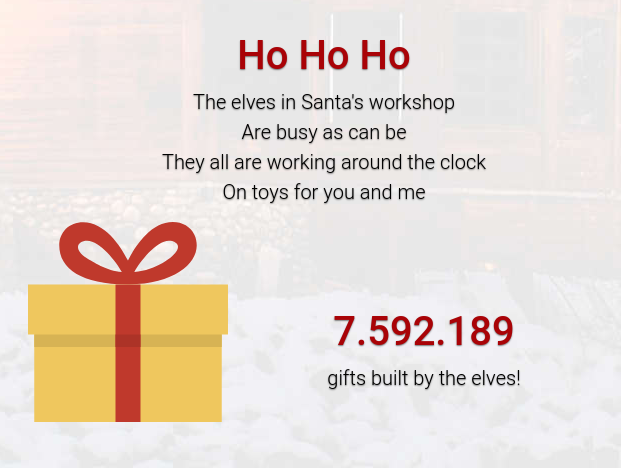
\includegraphics{./elves.png}
\caption{Website screenshot}
\end{figure}

Looking at the JavaScript source, we find a
\href{https://en.wikipedia.org/wiki/MQTT}{MQTT} connection used to
increment the counter. We also find out that the flag seems to be
published via MQTT as well:

\begin{Shaded}
\begin{Highlighting}[]
\KeywordTok{var}\NormalTok{ topic }\OperatorTok{=} \StringTok{\textquotesingle{}HV19/gifts/\textquotesingle{}}\OperatorTok{+}\NormalTok{clientid}\OperatorTok{;}
\CommentTok{// var topic = \textquotesingle{}HV19/gifts/\textquotesingle{}+clientid+\textquotesingle{}/flag{-}tbd\textquotesingle{};}
\end{Highlighting}
\end{Shaded}

I started with replicating what the website does in Python - I first
didn't get it to run, until I got a hint that I need to set
\texttt{transport="websockets"} for it to be equivalent with the
JavaScript code. I also added a counter so that the loop automatically
exits after getting 5 messages. I mainly use that to have a clean way to
exit the mainloop for this writeup.

After that, I got gift counter messages via Python and
\href{https://pypi.org/project/paho-mqtt/}{paho-mqtt}:

    \begin{tcolorbox}[breakable, size=fbox, boxrule=1pt, pad at break*=1mm,colback=cellbackground, colframe=cellborder]
\prompt{In}{incolor}{17}{\boxspacing}
\begin{Verbatim}[commandchars=\\\{\}]
\PY{k+kn}{import} \PY{n+nn}{logging}
\PY{k+kn}{import} \PY{n+nn}{paho}\PY{n+nn}{.}\PY{n+nn}{mqtt}\PY{n+nn}{.}\PY{n+nn}{client} \PY{k}{as} \PY{n+nn}{mqtt}
\PY{k+kn}{import} \PY{n+nn}{itertools}


\PY{n}{CID} \PY{o}{=} \PY{l+s+s2}{\PYZdq{}}\PY{l+s+s2}{0483191873374145}\PY{l+s+s2}{\PYZdq{}}
\PY{n}{USER} \PY{o}{=} \PY{l+s+s2}{\PYZdq{}}\PY{l+s+s2}{workshop}\PY{l+s+s2}{\PYZdq{}}
\PY{n}{PASS} \PY{o}{=} \PY{l+s+s2}{\PYZdq{}}\PY{l+s+s2}{2fXc7AWINBXyruvKLiX}\PY{l+s+s2}{\PYZdq{}}
\PY{n}{HOST} \PY{o}{=} \PY{l+s+s2}{\PYZdq{}}\PY{l+s+s2}{whale.hacking\PYZhy{}lab.com}\PY{l+s+s2}{\PYZdq{}}
\PY{n}{PORT} \PY{o}{=} \PY{l+m+mi}{9001}
\PY{n}{TOPIC} \PY{o}{=} \PY{l+s+sa}{f}\PY{l+s+s2}{\PYZdq{}}\PY{l+s+s2}{HV19/gifts/}\PY{l+s+si}{\PYZob{}CID\PYZcb{}}\PY{l+s+s2}{\PYZdq{}}
\PY{n}{LIMIT} \PY{o}{=} \PY{l+m+mi}{5}

\PY{n}{counter} \PY{o}{=} \PY{k+kc}{None}


\PY{k}{def} \PY{n+nf}{on\PYZus{}connect}\PY{p}{(}\PY{n}{client}\PY{p}{,} \PY{n}{userdata}\PY{p}{,} \PY{n}{flags}\PY{p}{,} \PY{n}{rc}\PY{p}{)}\PY{p}{:}
    \PY{k}{if} \PY{n}{rc} \PY{o}{!=} \PY{l+m+mi}{0}\PY{p}{:}
        \PY{n+nb}{print}\PY{p}{(}\PY{l+s+sa}{f}\PY{l+s+s2}{\PYZdq{}}\PY{l+s+s2}{Failed to connect: }\PY{l+s+si}{\PYZob{}rc\PYZcb{}}\PY{l+s+s2}{\PYZdq{}}\PY{p}{)}

    \PY{n}{client}\PY{o}{.}\PY{n}{subscribe}\PY{p}{(}\PY{n}{TOPIC}\PY{p}{)}
    
    \PY{k}{global} \PY{n}{counter}
    \PY{n}{counter} \PY{o}{=} \PY{n}{itertools}\PY{o}{.}\PY{n}{count}\PY{p}{(}\PY{n}{start}\PY{o}{=}\PY{l+m+mi}{1}\PY{p}{)}


\PY{k}{def} \PY{n+nf}{on\PYZus{}message}\PY{p}{(}\PY{n}{client}\PY{p}{,} \PY{n}{userdata}\PY{p}{,} \PY{n}{msg}\PY{p}{)}\PY{p}{:}
    \PY{n+nb}{print}\PY{p}{(}\PY{n}{msg}\PY{o}{.}\PY{n}{topic} \PY{o}{+} \PY{l+s+s2}{\PYZdq{}}\PY{l+s+s2}{ }\PY{l+s+s2}{\PYZdq{}} \PY{o}{+} \PY{n+nb}{str}\PY{p}{(}\PY{n}{msg}\PY{o}{.}\PY{n}{payload}\PY{p}{)}\PY{p}{)}
    \PY{k}{if} \PY{n+nb}{next}\PY{p}{(}\PY{n}{counter}\PY{p}{)} \PY{o}{==} \PY{n}{LIMIT}\PY{p}{:}
        \PY{n}{client}\PY{o}{.}\PY{n}{disconnect}\PY{p}{(}\PY{p}{)}

        
\PY{k}{def} \PY{n+nf}{run}\PY{p}{(}\PY{n}{client}\PY{p}{)}\PY{p}{:}
    \PY{n}{client}\PY{o}{.}\PY{n}{enable\PYZus{}logger}\PY{p}{(}\PY{p}{)}
    \PY{n}{logging}\PY{o}{.}\PY{n}{basicConfig}\PY{p}{(}\PY{n}{level}\PY{o}{=}\PY{n}{logging}\PY{o}{.}\PY{n}{DEBUG}\PY{p}{)}

    \PY{n}{client}\PY{o}{.}\PY{n}{username\PYZus{}pw\PYZus{}set}\PY{p}{(}\PY{n}{USER}\PY{p}{,} \PY{n}{PASS}\PY{p}{)}

    \PY{n}{client}\PY{o}{.}\PY{n}{on\PYZus{}connect} \PY{o}{=} \PY{n}{on\PYZus{}connect}
    \PY{n}{client}\PY{o}{.}\PY{n}{on\PYZus{}message} \PY{o}{=} \PY{n}{on\PYZus{}message}

    \PY{n}{client}\PY{o}{.}\PY{n}{connect}\PY{p}{(}\PY{n}{HOST}\PY{p}{,} \PY{n}{PORT}\PY{p}{)}

    \PY{n}{client}\PY{o}{.}\PY{n}{loop\PYZus{}forever}\PY{p}{(}\PY{p}{)}
    
\PY{n}{client} \PY{o}{=} \PY{n}{mqtt}\PY{o}{.}\PY{n}{Client}\PY{p}{(}\PY{n}{client\PYZus{}id}\PY{o}{=}\PY{n}{CID}\PY{p}{,} \PY{n}{transport}\PY{o}{=}\PY{l+s+s2}{\PYZdq{}}\PY{l+s+s2}{websockets}\PY{l+s+s2}{\PYZdq{}}\PY{p}{)}
\PY{n}{run}\PY{p}{(}\PY{n}{client}\PY{p}{)}
\end{Verbatim}
\end{tcolorbox}

    \begin{Verbatim}[commandchars=\\\{\}]
DEBUG:paho.mqtt.client:Sending CONNECT (u1, p1, wr0, wq0, wf0, c1, k60)
client\_id=b'0483191873374145'
DEBUG:paho.mqtt.client:Received CONNACK (0, 0)
DEBUG:paho.mqtt.client:Sending SUBSCRIBE (d0, m1)
[(b'HV19/gifts/0483191873374145', 0)]
DEBUG:paho.mqtt.client:Received SUBACK
DEBUG:paho.mqtt.client:Received PUBLISH (d0, q0, r0, m0),
'HV19/gifts/0483191873374145', {\ldots}  (7 bytes)
    \end{Verbatim}

    \begin{Verbatim}[commandchars=\\\{\}]
HV19/gifts/0483191873374145 b'7596557'
    \end{Verbatim}

    \begin{Verbatim}[commandchars=\\\{\}]
DEBUG:paho.mqtt.client:Received PUBLISH (d0, q0, r0, m0),
'HV19/gifts/0483191873374145', {\ldots}  (7 bytes)
    \end{Verbatim}

    \begin{Verbatim}[commandchars=\\\{\}]
HV19/gifts/0483191873374145 b'7596560'
    \end{Verbatim}

    \begin{Verbatim}[commandchars=\\\{\}]
DEBUG:paho.mqtt.client:Received PUBLISH (d0, q0, r0, m0),
'HV19/gifts/0483191873374145', {\ldots}  (7 bytes)
    \end{Verbatim}

    \begin{Verbatim}[commandchars=\\\{\}]
HV19/gifts/0483191873374145 b'7596569'
    \end{Verbatim}

    \begin{Verbatim}[commandchars=\\\{\}]
DEBUG:paho.mqtt.client:Received PUBLISH (d0, q0, r0, m0),
'HV19/gifts/0483191873374145', {\ldots}  (7 bytes)
    \end{Verbatim}

    \begin{Verbatim}[commandchars=\\\{\}]
HV19/gifts/0483191873374145 b'7596570'
    \end{Verbatim}

    \begin{Verbatim}[commandchars=\\\{\}]
DEBUG:paho.mqtt.client:Received PUBLISH (d0, q0, r0, m0),
'HV19/gifts/0483191873374145', {\ldots}  (7 bytes)
DEBUG:paho.mqtt.client:Sending DISCONNECT
    \end{Verbatim}

    \begin{Verbatim}[commandchars=\\\{\}]
HV19/gifts/0483191873374145 b'7596580'
    \end{Verbatim}

    I then did some reading about MQTT and found out that there are
wildcards using
\href{https://www.hivemq.com/blog/mqtt-essentials-part-5-mqtt-topics-best-practices/}{this
article}. Let's try to get everything!

    \begin{tcolorbox}[breakable, size=fbox, boxrule=1pt, pad at break*=1mm,colback=cellbackground, colframe=cellborder]
\prompt{In}{incolor}{18}{\boxspacing}
\begin{Verbatim}[commandchars=\\\{\}]
\PY{n}{TOPIC} \PY{o}{=} \PY{l+s+s2}{\PYZdq{}}\PY{l+s+s2}{\PYZsh{}}\PY{l+s+s2}{\PYZdq{}}
\PY{n}{client}\PY{o}{.}\PY{n}{connect}\PY{p}{(}\PY{n}{HOST}\PY{p}{,} \PY{n}{PORT}\PY{p}{)}
\PY{n}{client}\PY{o}{.}\PY{n}{loop\PYZus{}forever}\PY{p}{(}\PY{p}{)}
\end{Verbatim}
\end{tcolorbox}

    \begin{Verbatim}[commandchars=\\\{\}]
DEBUG:paho.mqtt.client:Sending CONNECT (u1, p1, wr0, wq0, wf0, c1, k60)
client\_id=b'0483191873374145'
DEBUG:paho.mqtt.client:Received CONNACK (0, 0)
DEBUG:paho.mqtt.client:Sending SUBSCRIBE (d0, m2) [(b'\#', 0)]
DEBUG:paho.mqtt.client:Received SUBACK
DEBUG:paho.mqtt.client:Received PUBLISH (d0, q0, r0, m0),
'HV19/gifts/0483191873374145', {\ldots}  (7 bytes)
    \end{Verbatim}

    \begin{Verbatim}[commandchars=\\\{\}]
HV19/gifts/0483191873374145 b'7596661'
    \end{Verbatim}

    \begin{Verbatim}[commandchars=\\\{\}]
DEBUG:paho.mqtt.client:Received PUBLISH (d0, q0, r0, m0),
'HV19/gifts/0483191873374145', {\ldots}  (7 bytes)
    \end{Verbatim}

    \begin{Verbatim}[commandchars=\\\{\}]
HV19/gifts/0483191873374145 b'7596664'
    \end{Verbatim}

    \begin{Verbatim}[commandchars=\\\{\}]
DEBUG:paho.mqtt.client:Received PUBLISH (d0, q0, r0, m0),
'HV19/gifts/0483191873374145', {\ldots}  (7 bytes)
    \end{Verbatim}

    \begin{Verbatim}[commandchars=\\\{\}]
HV19/gifts/0483191873374145 b'7596673'
    \end{Verbatim}

    \begin{Verbatim}[commandchars=\\\{\}]
DEBUG:paho.mqtt.client:Received PUBLISH (d0, q0, r0, m0),
'HV19/gifts/0483191873374145', {\ldots}  (7 bytes)
    \end{Verbatim}

    \begin{Verbatim}[commandchars=\\\{\}]
HV19/gifts/0483191873374145 b'7596677'
    \end{Verbatim}

    \begin{Verbatim}[commandchars=\\\{\}]
DEBUG:paho.mqtt.client:Received PUBLISH (d0, q0, r0, m0),
'HV19/gifts/0483191873374145', {\ldots}  (7 bytes)
DEBUG:paho.mqtt.client:Sending DISCONNECT
    \end{Verbatim}

    \begin{Verbatim}[commandchars=\\\{\}]
HV19/gifts/0483191873374145 b'7596686'
    \end{Verbatim}

            \begin{tcolorbox}[breakable, size=fbox, boxrule=.5pt, pad at break*=1mm, opacityfill=0]
\prompt{Out}{outcolor}{18}{\boxspacing}
\begin{Verbatim}[commandchars=\\\{\}]
7
\end{Verbatim}
\end{tcolorbox}
        
    Hmm, nothing new there. I'd have expected to also see gift messages for
other users at least, but I guess there are some access controls which
prevent that.

The article above mentions:

\begin{quote}
Topics that start with a \$ symbol have a different purpose. These
topics are not part of the subscription when you subscribe to the
multi-level wildcard as a topic (\#). \textbf{The \$-symbol topics are
reserved for internal statistics of the MQTT broker.}
\end{quote}

So let's check whether there's something interesting to see there!

    \begin{tcolorbox}[breakable, size=fbox, boxrule=1pt, pad at break*=1mm,colback=cellbackground, colframe=cellborder]
\prompt{In}{incolor}{19}{\boxspacing}
\begin{Verbatim}[commandchars=\\\{\}]
\PY{n}{TOPIC} \PY{o}{=} \PY{l+s+sa}{f}\PY{l+s+s2}{\PYZdq{}}\PY{l+s+s2}{\PYZdl{}SYS/\PYZsh{}}\PY{l+s+s2}{\PYZdq{}}
\PY{n}{LIMIT} \PY{o}{=} \PY{l+m+mi}{1}
\PY{n}{client}\PY{o}{.}\PY{n}{connect}\PY{p}{(}\PY{n}{HOST}\PY{p}{,} \PY{n}{PORT}\PY{p}{)}
\PY{n}{client}\PY{o}{.}\PY{n}{loop\PYZus{}forever}\PY{p}{(}\PY{p}{)}
\end{Verbatim}
\end{tcolorbox}

    \begin{Verbatim}[commandchars=\\\{\}]
DEBUG:paho.mqtt.client:Sending CONNECT (u1, p1, wr0, wq0, wf0, c1, k60)
client\_id=b'0483191873374145'
DEBUG:paho.mqtt.client:Received CONNACK (0, 0)
DEBUG:paho.mqtt.client:Sending SUBSCRIBE (d0, m3) [(b'\$SYS/\#', 0)]
DEBUG:paho.mqtt.client:Received PUBLISH (d0, q0, r1, m0), '\$SYS/broker/version',
{\ldots}  (157 bytes)
DEBUG:paho.mqtt.client:Sending DISCONNECT
DEBUG:paho.mqtt.client:Received SUBACK
    \end{Verbatim}

    \begin{Verbatim}[commandchars=\\\{\}]
\$SYS/broker/version b'mosquitto version 1.4.11 (We elves are super-smart and
know about CVE-2017-7650 and the POC. So we made a genious fix you never will be
able to pass. Hohoho)'
    \end{Verbatim}

            \begin{tcolorbox}[breakable, size=fbox, boxrule=.5pt, pad at break*=1mm, opacityfill=0]
\prompt{Out}{outcolor}{19}{\boxspacing}
\begin{Verbatim}[commandchars=\\\{\}]
7
\end{Verbatim}
\end{tcolorbox}
        
    Oh, that's interesting! The message informs us about
\href{http://cve.circl.lu/cve/CVE-2017-7650}{CVE-2017-7650}:

\begin{quote}
In Mosquitto before 1.4.12, pattern based ACLs can be bypassed by
clients that set their username/client id to `\#' or `+'. This allows
locally or remotely connected clients to access MQTT topics that they do
have the rights to.
\end{quote}

From the
\href{https://bugs.eclipse.org/bugs/show_bug.cgi?id=516765}{related bug
report} and the
\href{https://bugs.eclipse.org/bugs/attachment.cgi?id=268603}{attached
patch} we get some more information. The upstream patch seems fine, but
it looks like the elves fixed it in a different way, which apparently
can be circumvented somehow.

I first tried the obvious thing, a client ID of \texttt{\#}, but that
doesn't let us connect at all:

    \begin{tcolorbox}[breakable, size=fbox, boxrule=1pt, pad at break*=1mm,colback=cellbackground, colframe=cellborder]
\prompt{In}{incolor}{ }{\boxspacing}
\begin{Verbatim}[commandchars=\\\{\}]
\PY{n}{TOPIC} \PY{o}{=} \PY{l+s+s2}{\PYZdq{}}\PY{l+s+s2}{\PYZsh{}}\PY{l+s+s2}{\PYZdq{}}
\PY{n}{CID} \PY{o}{=} \PY{l+s+s2}{\PYZdq{}}\PY{l+s+s2}{\PYZsh{}}\PY{l+s+s2}{\PYZdq{}}

\PY{n}{client} \PY{o}{=} \PY{n}{mqtt}\PY{o}{.}\PY{n}{Client}\PY{p}{(}\PY{n}{client\PYZus{}id}\PY{o}{=}\PY{n}{CID}\PY{p}{,} \PY{n}{transport}\PY{o}{=}\PY{l+s+s2}{\PYZdq{}}\PY{l+s+s2}{websockets}\PY{l+s+s2}{\PYZdq{}}\PY{p}{)}
\PY{n}{run}\PY{p}{(}\PY{n}{client}\PY{p}{)}
\end{Verbatim}
\end{tcolorbox}

    The client ID is part of the published topic as well. So I did a guess -
what if I used \texttt{0483191873374145/\#} as client ID, so that
(maybe) the server sends to \texttt{HV19/gifts/0483191873374145/\#} or
so?

    \begin{tcolorbox}[breakable, size=fbox, boxrule=1pt, pad at break*=1mm,colback=cellbackground, colframe=cellborder]
\prompt{In}{incolor}{24}{\boxspacing}
\begin{Verbatim}[commandchars=\\\{\}]
\PY{n}{LIMIT} \PY{o}{=} \PY{l+m+mi}{5}
\PY{n}{CID} \PY{o}{=} \PY{l+s+s2}{\PYZdq{}}\PY{l+s+s2}{0483191873374145/\PYZsh{}}\PY{l+s+s2}{\PYZdq{}}
\PY{n}{client} \PY{o}{=} \PY{n}{mqtt}\PY{o}{.}\PY{n}{Client}\PY{p}{(}\PY{n}{client\PYZus{}id}\PY{o}{=}\PY{n}{CID}\PY{p}{,} \PY{n}{transport}\PY{o}{=}\PY{l+s+s2}{\PYZdq{}}\PY{l+s+s2}{websockets}\PY{l+s+s2}{\PYZdq{}}\PY{p}{)}
\PY{n}{run}\PY{p}{(}\PY{n}{client}\PY{p}{)}
\end{Verbatim}
\end{tcolorbox}

    \begin{Verbatim}[commandchars=\\\{\}]
DEBUG:paho.mqtt.client:Sending CONNECT (u1, p1, wr0, wq0, wf0, c1, k60)
client\_id=b'0483191873374145/\#'
DEBUG:paho.mqtt.client:Received CONNACK (0, 0)
DEBUG:paho.mqtt.client:Sending SUBSCRIBE (d0, m1) [(b'\#', 0)]
DEBUG:paho.mqtt.client:Received PUBLISH (d0, q0, r1, m0),
'HV19/gifts/0483191873374145/HV19\{N0\_1nput\_v4l1d4t10n\_3qu4ls\_d1s4st3r\}', {\ldots}
(70 bytes)
DEBUG:paho.mqtt.client:Received SUBACK
    \end{Verbatim}

    \begin{Verbatim}[commandchars=\\\{\}]
HV19/gifts/0483191873374145/HV19\{N0\_1nput\_v4l1d4t10n\_3qu4ls\_d1s4st3r\}
b'Congrats, you got it. The elves should not overrate their smartness!!!'
    \end{Verbatim}

    \begin{Verbatim}[commandchars=\\\{\}]
DEBUG:paho.mqtt.client:Received PUBLISH (d0, q0, r0, m0),
'HV19/gifts/0483191873374145/HV19\{N0\_1nput\_v4l1d4t10n\_3qu4ls\_d1s4st3r\}', {\ldots}
(70 bytes)
DEBUG:paho.mqtt.client:Received PUBLISH (d0, q0, r0, m0),
'HV19/gifts/0483191873374145', {\ldots}  (7 bytes)
    \end{Verbatim}

    \begin{Verbatim}[commandchars=\\\{\}]
HV19/gifts/0483191873374145/HV19\{N0\_1nput\_v4l1d4t10n\_3qu4ls\_d1s4st3r\}
b'Congrats, you got it. The elves should not overrate their smartness!!!'
HV19/gifts/0483191873374145 b'7599123'
    \end{Verbatim}

    \begin{Verbatim}[commandchars=\\\{\}]
DEBUG:paho.mqtt.client:Received PUBLISH (d0, q0, r0, m0),
'HV19/gifts/0483191873374145/HV19\{N0\_1nput\_v4l1d4t10n\_3qu4ls\_d1s4st3r\}', {\ldots}
(70 bytes)
DEBUG:paho.mqtt.client:Received PUBLISH (d0, q0, r0, m0),
'HV19/gifts/0483191873374145', {\ldots}  (7 bytes)
DEBUG:paho.mqtt.client:Sending DISCONNECT
    \end{Verbatim}

    \begin{Verbatim}[commandchars=\\\{\}]
HV19/gifts/0483191873374145/HV19\{N0\_1nput\_v4l1d4t10n\_3qu4ls\_d1s4st3r\}
b'Congrats, you got it. The elves should not overrate their smartness!!!'
HV19/gifts/0483191873374145 b'7599128'
    \end{Verbatim}

    And indeed, the flag is
\texttt{HV19\{N0\_1nput\_v4l1d4t10n\_3qu4ls\_d1s4st3r\}}.



    
\pagebreak{}
    \hypertarget{hv19.16-b0rked-calculator}{%
\section{HV19.16 B0rked Calculator}\label{hv19.16-b0rked-calculator}}

\emph{Santa has coded a simple project for you, but sadly he removed all
the operations. But when you restore them it will print the flag!}

We get an \texttt{.exe} file - thankfully it runs fine under
\href{https://www.winehq.org/}{Wine}, as I prefer to work on Linux
without a Windows VM when possible:

\begin{figure}
\centering
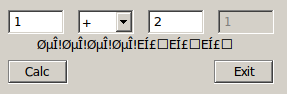
\includegraphics{./calc.png}
\caption{Calculator screenshot}
\end{figure}

Other than the ``Back to basic'' nightmare earlier this Hackvent, this
was the first time I reverse-engineered a binary. I already had
\href{https://ghidra-sre.org/}{Ghidra} installed on my machine, but
never used it so far. So I opened the exe in Ghidra to take a closer
look!

At address \texttt{0040145b} (in what's probably the \texttt{main}
function), we find (slightly edited):

\begin{Shaded}
\begin{Highlighting}[]
\ControlFlowTok{if}\NormalTok{ (DAT\_00402138 == }\CharTok{\textquotesingle{}+\textquotesingle{}}\NormalTok{) \{}
\NormalTok{    uValue = FUN\_004015b6((}\DataTypeTok{char}\NormalTok{)uValue,}
\NormalTok{                          extraout\_DL\_02,}
\NormalTok{                          extraout\_CL\_02,}
\NormalTok{                          DAT\_00402120);}
\NormalTok{\} }\ControlFlowTok{else} \ControlFlowTok{if}\NormalTok{ (DAT\_00402138 == }\CharTok{\textquotesingle{}{-}\textquotesingle{}}\NormalTok{) \{}
\NormalTok{    uValue = FUN\_004015c4((}\DataTypeTok{char}\NormalTok{)uValue,}
\NormalTok{                          extraout\_DL\_02,}
\NormalTok{                          extraout\_CL\_02,}
\NormalTok{                          (}\DataTypeTok{char}\NormalTok{)DAT\_00402120,}
\NormalTok{                          uValue);}
\NormalTok{\} }\ControlFlowTok{else} \ControlFlowTok{if}\NormalTok{ (DAT\_00402138 == }\CharTok{\textquotesingle{}*\textquotesingle{}}\NormalTok{) \{}
\NormalTok{    uValue = FUN\_004015d4();}
\NormalTok{\} }\ControlFlowTok{else} \ControlFlowTok{if}\NormalTok{ (DAT\_00402138 == }\CharTok{\textquotesingle{}/\textquotesingle{}}\NormalTok{) \{}
\NormalTok{    uValue = FUN\_004015e4();}
\NormalTok{\}}
\end{Highlighting}
\end{Shaded}

So I renamed those functions to \texttt{op\_plus}, \texttt{op\_minus},
\texttt{op\_times} and \texttt{op\_divide}. They all look something like
this:

\begin{verbatim}
004015b6 c8 00 00 00     ENTER      0x0,0x0
004015ba 8b 45 08        MOV        param_1,dword ptr [EBP + param_4]
004015bd 90              NOP
004015be 90              NOP
004015bf 90              NOP
004015c0 c9              LEAVE
004015c1 c2 08 00        RET        0x8
\end{verbatim}

It looks like we're supposed to patch the binary so the calculator works
and the flag is shown. Unfortunately, Ghidra
\href{https://github.com/NationalSecurityAgency/ghidra/issues/19}{can't
save patched files} (unless they're opened as raw binary, which seems to
disable many useful analysis features). I found a
\href{https://github.com/schlafwandler/ghidra_SavePatch}{SavePatch.py
script} which seems to work fine.

However, I was a bit confused about the calling convention at that point
- where do I get the arguments, which registers can I use, and how do I
need to return the result?

I decided to dig a bit deeper - looking at references, we also find a
function I call \texttt{show\_flag} at \texttt{00401519}:

\begin{verbatim}
ENTER      0x0,0x0

PUSH       0x1762a070
PUSH       0x21ceb5d8
CALL       op_plus
MOV        [DAT_004020a0],param_1

PUSH       0x38b57698
PUSH       0xaae5b913
CALL       op_minus
MOV        [DAT_004020a4],param_1

PUSH       0x2
PUSH       0xbec8cad6
CALL       op_divide
MOV        [DAT_004020a8],param_1

PUSH       0x2
PUSH       0x33b0b623
CALL       op_times
MOV        [DAT_004020ac],param_1

PUSH       0x53bd761a
PUSH       0x18a3cd45
CALL       op_plus
MOV        [DAT_004020b0],param_1

PUSH       0x46c920f4
PUSH       0xa8359657
CALL       op_minus
MOV        [DAT_004020b4],param_1

PUSH       0x4
PUSH       0x1f5c8c1d
CALL       op_times
MOV        [DAT_004020b8],param_1

PUSH       DAT_004020a0
PUSH       0x3e8
PUSH       dword ptr [EBP + param_4]
CALL       SetDlgItemTextA

LEAVE
RET        0x4
\end{verbatim}

Since those oparations seemed quite straightforward, I thought I'd
instead reimplement them in Python instead.

If we look at the displayed flag, it starts with \texttt{صÎ!}. Encoded
as \href{https://de.wikipedia.org/wiki/ISO_8859-1}{Latin1} that'd be:
0xD8, 0xB5, 0xCE, 0x21

This matches up with the \texttt{0x21ceb5d8} above after some
bit-twiddling. Let's write a decoding function:

    \begin{tcolorbox}[breakable, size=fbox, boxrule=1pt, pad at break*=1mm,colback=cellbackground, colframe=cellborder]
\prompt{In}{incolor}{11}{\boxspacing}
\begin{Verbatim}[commandchars=\\\{\}]
\PY{k}{def} \PY{n+nf}{decode}\PY{p}{(}\PY{n}{dword}\PY{p}{)}\PY{p}{:}
    \PY{n}{data} \PY{o}{=} \PY{n}{dword}\PY{o}{.}\PY{n}{to\PYZus{}bytes}\PY{p}{(}\PY{l+m+mi}{4}\PY{p}{,} \PY{n}{byteorder}\PY{o}{=}\PY{l+s+s1}{\PYZsq{}}\PY{l+s+s1}{little}\PY{l+s+s1}{\PYZsq{}}\PY{p}{)}
    \PY{k}{return} \PY{n}{data}\PY{o}{.}\PY{n}{decode}\PY{p}{(}\PY{l+s+s1}{\PYZsq{}}\PY{l+s+s1}{latin1}\PY{l+s+s1}{\PYZsq{}}\PY{p}{)}

\PY{n+nb}{print}\PY{p}{(}\PY{n}{decode}\PY{p}{(}\PY{l+m+mh}{0x21ceb5d8}\PY{p}{)}\PY{p}{)}
\end{Verbatim}
\end{tcolorbox}

    \begin{Verbatim}[commandchars=\\\{\}]
صÎ!
    \end{Verbatim}

    Then we can get the flag by reimplementing the same calculations in
Python:

    \begin{tcolorbox}[breakable, size=fbox, boxrule=1pt, pad at break*=1mm,colback=cellbackground, colframe=cellborder]
\prompt{In}{incolor}{14}{\boxspacing}
\begin{Verbatim}[commandchars=\\\{\}]
\PY{n}{flag} \PY{o}{=} \PY{n}{decode}\PY{p}{(}\PY{l+m+mh}{0x21ceb5d8} \PY{o}{+} \PY{l+m+mh}{0x1762a070}\PY{p}{)}
\PY{n}{flag} \PY{o}{+}\PY{o}{=} \PY{n}{decode}\PY{p}{(}\PY{l+m+mh}{0xaae5b913} \PY{o}{\PYZhy{}} \PY{l+m+mh}{0x38b57698}\PY{p}{)}
\PY{n}{flag} \PY{o}{+}\PY{o}{=} \PY{n}{decode}\PY{p}{(}\PY{l+m+mh}{0xbec8cad6} \PY{o}{/}\PY{o}{/} \PY{l+m+mi}{2}\PY{p}{)}
\PY{n}{flag} \PY{o}{+}\PY{o}{=} \PY{n}{decode}\PY{p}{(}\PY{l+m+mh}{0x33b0b623} \PY{o}{*} \PY{l+m+mi}{2}\PY{p}{)}
\PY{n}{flag} \PY{o}{+}\PY{o}{=} \PY{n}{decode}\PY{p}{(}\PY{l+m+mh}{0x53bd761a} \PY{o}{+} \PY{l+m+mh}{0x18a3cd45}\PY{p}{)}
\PY{n}{flag} \PY{o}{+}\PY{o}{=} \PY{n}{decode}\PY{p}{(}\PY{l+m+mh}{0xa8359657} \PY{o}{\PYZhy{}} \PY{l+m+mh}{0x46c920f4}\PY{p}{)}
\PY{n}{flag} \PY{o}{+}\PY{o}{=} \PY{n}{decode}\PY{p}{(}\PY{l+m+mh}{0x1f5c8c1d} \PY{o}{*} \PY{l+m+mi}{4}\PY{p}{)}
\PY{n+nb}{print}\PY{p}{(}\PY{n}{flag}\PY{p}{)}
\end{Verbatim}
\end{tcolorbox}

    \begin{Verbatim}[commandchars=\\\{\}]
HV19\{B0rked\_Flag\_Calculat0r\}
    \end{Verbatim}



    
\pagebreak{}
    \hypertarget{hv19.17-unicode-portal}{%
\section{HV19.17 Unicode Portal}\label{hv19.17-unicode-portal}}

\emph{Buy your special gifts online, but for the ultimative gift you
have to become admin.}

In this challenge, we get a web portal focused on unicode characters:

\begin{figure}
\centering

\includegraphics{./portal.png}
\caption{Portal screenshot}
\end{figure}

After registering an account and logging in, we can access a ``Source''
page: \emph{Since Santa is a big fan of open source software, he
publicly provides his authentication code. For free!}.

From there, we can get this PHP snippet:

\begin{Shaded}
\begin{Highlighting}[]
\KeywordTok{<?php}

\KeywordTok{if} \OtherTok{(}\KeywordTok{isset}\OtherTok{(}\KeywordTok{$\_GET}\OtherTok{[}\StringTok{\textquotesingle{}show\textquotesingle{}}\OtherTok{]))} \FunctionTok{highlight\_file}\OtherTok{(}\KeywordTok{\_\_FILE\_\_}\OtherTok{);}

\CommentTok{/**}
\CommentTok{ * Verifies user credentials.}
\CommentTok{ */}
\KeywordTok{function}\NormalTok{ verifyCreds}\OtherTok{(}\KeywordTok{$conn}\OtherTok{,} \KeywordTok{$username}\OtherTok{,} \KeywordTok{$password}\OtherTok{)}\NormalTok{ \{}
  \KeywordTok{$usr}\NormalTok{ = }\KeywordTok{$conn}\NormalTok{{-}>real\_escape\_string}\OtherTok{(}\KeywordTok{$username}\OtherTok{);}
  \KeywordTok{$res}\NormalTok{ = }\KeywordTok{$conn}\NormalTok{{-}>query}\OtherTok{(}\StringTok{"SELECT password FROM users WHERE username=\textquotesingle{}"}\NormalTok{.}\KeywordTok{$usr}\NormalTok{.}\StringTok{"\textquotesingle{}"}\OtherTok{);}
  \KeywordTok{$row}\NormalTok{ = }\KeywordTok{$res}\NormalTok{{-}>fetch\_assoc}\OtherTok{();}
  \KeywordTok{if} \OtherTok{(}\KeywordTok{$row}\OtherTok{)}\NormalTok{ \{}
    \KeywordTok{if} \OtherTok{(}\FunctionTok{password\_verify}\OtherTok{(}\KeywordTok{$password}\OtherTok{,} \KeywordTok{$row}\OtherTok{[}\StringTok{\textquotesingle{}password\textquotesingle{}}\OtherTok{]))} \KeywordTok{return} \KeywordTok{true}\OtherTok{;}
    \KeywordTok{else}\NormalTok{ addFailedLoginAttempt}\OtherTok{(}\KeywordTok{$conn}\OtherTok{,} \KeywordTok{$\_SERVER}\OtherTok{[}\StringTok{\textquotesingle{}REMOTE\_ADDR\textquotesingle{}}\OtherTok{]);}
\NormalTok{  \}}
  \KeywordTok{return} \KeywordTok{false}\OtherTok{;}
\NormalTok{\}}

\CommentTok{/**}
\CommentTok{ * Determines if the given user is admin.}
\CommentTok{ */}
\KeywordTok{function}\NormalTok{ isAdmin}\OtherTok{(}\KeywordTok{$username}\OtherTok{)}\NormalTok{ \{}
  \KeywordTok{return} \OtherTok{(}\KeywordTok{$username}\NormalTok{ === }\StringTok{\textquotesingle{}santa\textquotesingle{}}\OtherTok{);}
\NormalTok{\}}

\CommentTok{/**}
\CommentTok{ * Determines if the given username is already taken.}
\CommentTok{ */}
\KeywordTok{function}\NormalTok{ isUsernameAvailable}\OtherTok{(}\KeywordTok{$conn}\OtherTok{,} \KeywordTok{$username}\OtherTok{)}\NormalTok{ \{}
  \KeywordTok{$usr}\NormalTok{ = }\KeywordTok{$conn}\NormalTok{{-}>real\_escape\_string}\OtherTok{(}\KeywordTok{$username}\OtherTok{);}
  \KeywordTok{$res}\NormalTok{ = }\KeywordTok{$conn}\NormalTok{{-}>query}\OtherTok{(}\StringTok{"SELECT COUNT(*) AS cnt FROM users}
\StringTok{WHERE LOWER(username) = BINARY LOWER(\textquotesingle{}"}\NormalTok{.}\KeywordTok{$usr}\NormalTok{.}\StringTok{"\textquotesingle{})"}\OtherTok{);}
  \KeywordTok{$row}\NormalTok{ = }\KeywordTok{$res}\NormalTok{{-}>fetch\_assoc}\OtherTok{();}
  \KeywordTok{return} \DataTypeTok{(int)}\KeywordTok{$row}\OtherTok{[}\StringTok{\textquotesingle{}cnt\textquotesingle{}}\OtherTok{]}\NormalTok{ === }\DecValTok{0}\OtherTok{;}
\NormalTok{\}}

\CommentTok{/**}
\CommentTok{ * Registers a new user.}
\CommentTok{ */}
\KeywordTok{function}\NormalTok{ registerUser}\OtherTok{(}\KeywordTok{$conn}\OtherTok{,} \KeywordTok{$username}\OtherTok{,} \KeywordTok{$password}\OtherTok{)}\NormalTok{ \{}
  \KeywordTok{$usr}\NormalTok{ = }\KeywordTok{$conn}\NormalTok{{-}>real\_escape\_string}\OtherTok{(}\KeywordTok{$username}\OtherTok{);}
  \KeywordTok{$pwd}\NormalTok{ = }\FunctionTok{password\_hash}\OtherTok{(}\KeywordTok{$password}\OtherTok{,} \KeywordTok{PASSWORD\_DEFAULT}\OtherTok{);}
  \KeywordTok{$conn}\NormalTok{{-}>query}\OtherTok{(}\StringTok{"INSERT INTO users (username, password) VALUES}
\StringTok{(UPPER(\textquotesingle{}"}\NormalTok{.}\KeywordTok{$usr}\NormalTok{.}\StringTok{"\textquotesingle{}),\textquotesingle{}"}\NormalTok{.}\KeywordTok{$pwd}\NormalTok{.}\StringTok{"\textquotesingle{}) ON DUPLICATE KEY UPDATE password=\textquotesingle{}"}\NormalTok{.}\KeywordTok{$pwd}\NormalTok{.}\StringTok{"\textquotesingle{}"}\OtherTok{);}
\NormalTok{\}}

\CommentTok{/**}
\CommentTok{ * Adds a failed login attempt for the given ip address. An ip address gets}
\CommentTok{blacklisted for 15 minutes if there are more than 3 failed login attempts.}
\CommentTok{ */}
\KeywordTok{function}\NormalTok{ addFailedLoginAttempt}\OtherTok{(}\KeywordTok{$conn}\OtherTok{,} \KeywordTok{$ip}\OtherTok{)}\NormalTok{ \{}
  \KeywordTok{$ip}\NormalTok{ = }\KeywordTok{$conn}\NormalTok{{-}>real\_escape\_string}\OtherTok{(}\KeywordTok{$ip}\OtherTok{);}
  \KeywordTok{$conn}\NormalTok{{-}>query}\OtherTok{(}\StringTok{"INSERT INTO fails (ip) VALUES (\textquotesingle{}"}\NormalTok{.}\KeywordTok{$ip}\NormalTok{.}\StringTok{"\textquotesingle{})"}\OtherTok{);}
\NormalTok{\}}

\KeywordTok{?>}
\end{Highlighting}
\end{Shaded}

I can't see any SQL injection or obvious PHP issues (like using
\texttt{==} instead of \texttt{===}) there, but there are some things
that seem strange:

\begin{itemize}
\tightlist
\item
  We can access the ``admin'' page (which probably gives us the flag) if
  we can log in as the ``santa'' user.
\item
  If \texttt{registerUser} gets called with a duplicate key, it updates
  the password of santa.
\item
  The \texttt{registerUser} function calls \texttt{UPPER(...)} on the
  username
\item
  However, we're prevented from registering an existing user due to the
  check in \texttt{isUsernameAvailable}
\item
  Note that that function uses
  \texttt{LOWER(...)\ =\ BINARY\ LOWER(...)} to check for usernames.
\end{itemize}

At that point I was pretty sure this was related to case handling
somehow. For \texttt{a-z}/\texttt{A-Z}, the mapping from lower- to
uppercase is quite obvious. However, the challenge makes it obvious that
we'll need to deal with Unicode somehow. In alphabets other than the
typical English/latin alphabet, things can get hairy.

The typical example of this is probably
\href{http://www.i18nguy.com/unicode/turkish-i18n.html}{Turkish}: Their
alphabet has lower-/uppercase version of a dotless i (ı/I) and a dotted
i (i/İ). Those are different sounds - in other words, upper/lowercasing
words in a non locale-aware way results in a wrong word:

    \begin{tcolorbox}[breakable, size=fbox, boxrule=1pt, pad at break*=1mm,colback=cellbackground, colframe=cellborder]
\prompt{In}{incolor}{1}{\boxspacing}
\begin{Verbatim}[commandchars=\\\{\}]
\PY{l+s+s2}{\PYZdq{}}\PY{l+s+s2}{Kadın}\PY{l+s+s2}{\PYZdq{}}\PY{o}{.}\PY{n}{upper}\PY{p}{(}\PY{p}{)}\PY{o}{.}\PY{n}{lower}\PY{p}{(}\PY{p}{)}
\end{Verbatim}
\end{tcolorbox}

            \begin{tcolorbox}[breakable, size=fbox, boxrule=.5pt, pad at break*=1mm, opacityfill=0]
\prompt{Out}{outcolor}{1}{\boxspacing}
\begin{Verbatim}[commandchars=\\\{\}]
'kadin'
\end{Verbatim}
\end{tcolorbox}
        
    This issue recently caused a
\href{https://eng.getwisdom.io/hacking-github-with-unicode-dotless-i/}{security
bug} on GitHub! We can get something similar with the German ß as well:

    \begin{tcolorbox}[breakable, size=fbox, boxrule=1pt, pad at break*=1mm,colback=cellbackground, colframe=cellborder]
\prompt{In}{incolor}{2}{\boxspacing}
\begin{Verbatim}[commandchars=\\\{\}]
\PY{l+s+s2}{\PYZdq{}}\PY{l+s+s2}{Straße}\PY{l+s+s2}{\PYZdq{}}\PY{o}{.}\PY{n}{upper}\PY{p}{(}\PY{p}{)}\PY{o}{.}\PY{n}{lower}\PY{p}{(}\PY{p}{)}
\end{Verbatim}
\end{tcolorbox}

            \begin{tcolorbox}[breakable, size=fbox, boxrule=.5pt, pad at break*=1mm, opacityfill=0]
\prompt{Out}{outcolor}{2}{\boxspacing}
\begin{Verbatim}[commandchars=\\\{\}]
'strasse'
\end{Verbatim}
\end{tcolorbox}
        
    To change the password of santa, we'll need to find something that
passes as ``santa'' when registering (thus changing the password of the
santa user), but doesn't get detected by \texttt{isUsernameAvailable}.

Since I wasn't exactly sure how those casing collisions work in
practice, I started by reading the
\href{http://unicode.org/faq/casemap_charprop.html}{Unicode case mapping
FAQ}. There, a question caught my attention:

\begin{quote}
Q: Why is there no unique uppercase character for ſ --- U+017F LATIN
SMALL LETTER LONG S (and about one hundred other characters)?
\end{quote}

The \href{https://en.wikipedia.org/wiki/Long_s}{history of this
character} was quite an interesting read for the linguistics/typography
nerd in me!

Anyways - that character sounds like something we could use to create a
fake santa user:

    \begin{tcolorbox}[breakable, size=fbox, boxrule=1pt, pad at break*=1mm,colback=cellbackground, colframe=cellborder]
\prompt{In}{incolor}{3}{\boxspacing}
\begin{Verbatim}[commandchars=\\\{\}]
\PY{l+s+s2}{\PYZdq{}}\PY{l+s+s2}{ſanta}\PY{l+s+s2}{\PYZdq{}}\PY{o}{.}\PY{n}{upper}\PY{p}{(}\PY{p}{)}
\end{Verbatim}
\end{tcolorbox}

            \begin{tcolorbox}[breakable, size=fbox, boxrule=.5pt, pad at break*=1mm, opacityfill=0]
\prompt{Out}{outcolor}{3}{\boxspacing}
\begin{Verbatim}[commandchars=\\\{\}]
'SANTA'
\end{Verbatim}
\end{tcolorbox}
        
    And indeed, after registering a ``ſanta'' user, we can then log in as
``santa'' with the password we selected. Then, we can access the admin
page and get the flag, \texttt{HV19\{h4v1ng\_fun\_w1th\_un1c0d3\}}.


    
\pagebreak{}
    \hypertarget{hv19.h1-hidden-one}{%
\section{HV19.H1 Hidden One}\label{hv19.h1-hidden-one}}

This challenge was released on the same day ``HV19.06 bacon and eggs''
was, so let's take a closer look there.

Something seems strange - why is a code block used for some information
about Francis Bacon?

\begin{figure}
\centering

\includegraphics{codeblock.png}
\caption{Code block}
\end{figure}

Pressing ``copy to clipboard'' and pasting it into a file gives us the
same info:

    \begin{tcolorbox}[breakable, size=fbox, boxrule=1pt, pad at break*=1mm,colback=cellbackground, colframe=cellborder]
\prompt{In}{incolor}{3}{\boxspacing}
\begin{Verbatim}[commandchars=\\\{\}]
\PY{o}{\PYZpc{}}\PY{k}{cat} text.txt
\end{Verbatim}
\end{tcolorbox}

    \begin{Verbatim}[commandchars=\\\{\}]
Born: January 22
Died: April 9
Mother: Lady Anne
Father: Sir Nicholas
Secrets: unknown
    \end{Verbatim}

    However, when taking a closer look, we can see a mixture of whitespace
there. That sure seems strange!

    \begin{tcolorbox}[breakable, size=fbox, boxrule=1pt, pad at break*=1mm,colback=cellbackground, colframe=cellborder]
\prompt{In}{incolor}{4}{\boxspacing}
\begin{Verbatim}[commandchars=\\\{\}]
\PY{o}{!}hexdump \PYZhy{}C text.txt
\end{Verbatim}
\end{tcolorbox}

    \begin{Verbatim}[commandchars=\\\{\}]
00000000  42 6f 72 6e 3a 20 4a 61  6e 75 61 72 79 20 32 32  |Born: January 22|
00000010  09 20 20 20 20 20 09 20  09 20 20 20 09 20 20 20  |.     . .   .   |
00000020  09 20 09 20 20 20 20 20  20 20 09 20 20 20 20 20  |. .       .     |
00000030  09 20 20 09 20 20 0a 44  69 65 64 3a 20 41 70 72  |.  .  .Died: Apr|
00000040  69 6c 20 39 20 20 20 09  20 20 09 20 09 20 20 20  |il 9   .  . .   |
00000050  20 09 20 20 09 20 20 20  20 20 20 09 20 20 20 09  | .  .      .   .|
00000060  09 20 20 09 20 20 0a 4d  6f 74 68 65 72 3a 20 4c  |.  .  .Mother: L|
00000070  61 64 79 20 41 6e 6e 65  20 20 20 09 09 20 09 20  |ady Anne   .. . |
00000080  20 20 09 20 20 20 09 20  20 20 20 20 20 09 20 20  |  .   .      .  |
00000090  09 20 20 20 20 20 20 09  20 20 0a 46 61 74 68 65  |.      .  .Fathe|
000000a0  72 3a 20 53 69 72 20 4e  69 63 68 6f 6c 61 73 09  |r: Sir Nicholas.|
000000b0  20 09 20 20 20 20 20 20  09 09 20 20 20 20 09 20  | .      ..    . |
000000c0  20 20 20 09 20 20 09 20  20 09 20 20 20 20 20 20  |   .  .  .      |
000000d0  09 20 20 20 20 20 20 0a  53 65 63 72 65 74 73 3a  |.      .Secrets:|
000000e0  20 75 6e 6b 6e 6f 77 6e  20 20 20 20 20 20 09 20  | unknown      . |
000000f0  09 20 20 09 20 09 20 20  20 20 09 20 20 20 20 09  |.  . .    .    .|
00000100  20 20 20 09 20 20 20 20  20 20 20 09 20 20 0a     |   .       .  .|
0000010f
    \end{Verbatim}

    I first assumed the tabs/spaces would be another bacon cipher (like in
the original challenge), but that wasn't the case. Hiding data via
steganography with whitespace sure seems like a nice idea though. After
some quick research I found \href{http://darkside.com.au/snow/}{SNOW}:

\begin{quote}
The program SNOW is used to conceal messages in ASCII text by appending
whitespace to the end of lines. Because spaces and tabs are generally
not visible in text viewers, the message is effectively hidden from
casual observers.
\end{quote}

That sounds great. Let's give it a try!

    \begin{tcolorbox}[breakable, size=fbox, boxrule=1pt, pad at break*=1mm,colback=cellbackground, colframe=cellborder]
\prompt{In}{incolor}{6}{\boxspacing}
\begin{Verbatim}[commandchars=\\\{\}]
\PY{o}{!}snow text.txt
\end{Verbatim}
\end{tcolorbox}

    \begin{Verbatim}[commandchars=\\\{\}]
Warning: residual of 5 bits not output
<some binary output here>
    \end{Verbatim}

    Argh. Maybe that was too good to be true? Looking at the
\href{http://darkside.com.au/snow/manual.html}{manpage}, there are only
two options which affect decryption:

\begin{quote}
-C Compress the data if concealing, or uncompress it if extracting.

-p password If this is set, the data will be encrypted with this
password during concealment, or decrypted during extraction.
\end{quote}

I assume we don't need to guess/bruteforce a password. Let's try if the
compression flag helps (spoiler: it does!).

    \begin{tcolorbox}[breakable, size=fbox, boxrule=1pt, pad at break*=1mm,colback=cellbackground, colframe=cellborder]
\prompt{In}{incolor}{7}{\boxspacing}
\begin{Verbatim}[commandchars=\\\{\}]
\PY{o}{!}snow \PYZhy{}C text.txt
\end{Verbatim}
\end{tcolorbox}

    \begin{Verbatim}[commandchars=\\\{\}]
HV19\{1stHiddenFound\}
    \end{Verbatim}



    
\pagebreak{}
    \hypertarget{hv19.h2-hidden-two}{%
\section{HV19.H2 Hidden Two}\label{hv19.h2-hidden-two}}

This hidden challenge was released on the same day ``HV19.07 Santa
Rider'' was, so let's take a closer look at that challenge again.

The video in the challenge doesn't contain any audio, and I also
couldn't see anything hidden in the frames. However, it's downloadable
as a .zip file. Let's take a closer look at that zip!

    \begin{tcolorbox}[breakable, size=fbox, boxrule=1pt, pad at break*=1mm,colback=cellbackground, colframe=cellborder]
\prompt{In}{incolor}{2}{\boxspacing}
\begin{Verbatim}[commandchars=\\\{\}]
\PY{o}{!}unzip \PYZhy{}l video.zip
\end{Verbatim}
\end{tcolorbox}

    \begin{Verbatim}[commandchars=\\\{\}]
Archive:  video.zip
  Length      Date    Time    Name
---------  ---------- -----   ----
  2612690  2019-12-06 22:04   3DULK2N7DcpXFg8qGo9Z9qEQqvaEDpUCBB1v.mp4
---------                     -------
  2612690                     1 file
    \end{Verbatim}

    That filename seems weird, it's different from the usual
(autogenerated?) hex-filenames. Could it be base64?

    \begin{tcolorbox}[breakable, size=fbox, boxrule=1pt, pad at break*=1mm,colback=cellbackground, colframe=cellborder]
\prompt{In}{incolor}{6}{\boxspacing}
\begin{Verbatim}[commandchars=\\\{\}]
\PY{k+kn}{import} \PY{n+nn}{base64}
\PY{n}{base64}\PY{o}{.}\PY{n}{b64decode}\PY{p}{(}\PY{l+s+s2}{\PYZdq{}}\PY{l+s+s2}{3DULK2N7DcpXFg8qGo9Z9qEQqvaEDpUCBB1v}\PY{l+s+s2}{\PYZdq{}}\PY{p}{)}
\end{Verbatim}
\end{tcolorbox}

            \begin{tcolorbox}[breakable, size=fbox, boxrule=.5pt, pad at break*=1mm, opacityfill=0]
\prompt{Out}{outcolor}{6}{\boxspacing}
\begin{Verbatim}[commandchars=\\\{\}]
b'\textbackslash{}xdc5\textbackslash{}x0b+c\{\textbackslash{}r\textbackslash{}xcaW\textbackslash{}x16\textbackslash{}x0f*\textbackslash{}x1a\textbackslash{}x8fY\textbackslash{}xf6\textbackslash{}xa1\textbackslash{}x10\textbackslash{}xaa\textbackslash{}xf6\textbackslash{}x84\textbackslash{}x0e\textbackslash{}x95\textbackslash{}x02\textbackslash{}x04\textbackslash{}
x1do'
\end{Verbatim}
\end{tcolorbox}
        
    Hmm, nope. What other
\href{https://en.wikipedia.org/wiki/Binary-to-text_encoding\#Encoding_standards}{encodings
are there} where this character set would make sense?

It contains digits, lowercase and uppercase characters, but not anything
else. Assuming one of those common encodings, anything baseX with X
\textless{} 62 is out of the question. The chances of it being base85
but not containing any special chars are pretty slim.

Let's try \href{https://en.wikipedia.org/wiki/Base58}{base58}:
\emph{Base58 is a group of binary-to-text encoding schemes used to
represent large integers as alphanumeric text, introduced by Satoshi
Nakamoto for use with Bitcoin. It has since been applied to other
cryptocurrencies and applications. It is similar to Base64 but has been
modified to avoid both non-alphanumeric characters and letters which
might look ambiguous when printed.}

Thankfully, there's a \href{https://github.com/keis/base58}{Python
package} we can use.

    \begin{tcolorbox}[breakable, size=fbox, boxrule=1pt, pad at break*=1mm,colback=cellbackground, colframe=cellborder]
\prompt{In}{incolor}{9}{\boxspacing}
\begin{Verbatim}[commandchars=\\\{\}]
\PY{k+kn}{import} \PY{n+nn}{base58}
\PY{n+nb}{print}\PY{p}{(}\PY{n}{base58}\PY{o}{.}\PY{n}{b58decode}\PY{p}{(}\PY{l+s+s2}{\PYZdq{}}\PY{l+s+s2}{3DULK2N7DcpXFg8qGo9Z9qEQqvaEDpUCBB1v}\PY{l+s+s2}{\PYZdq{}}\PY{p}{)}\PY{o}{.}\PY{n}{decode}\PY{p}{(}\PY{l+s+s1}{\PYZsq{}}\PY{l+s+s1}{ascii}\PY{l+s+s1}{\PYZsq{}}\PY{p}{)}\PY{p}{)}
\end{Verbatim}
\end{tcolorbox}

    \begin{Verbatim}[commandchars=\\\{\}]
HV19\{Dont\_confuse\_0\_and\_O\}
    \end{Verbatim}


    
\pagebreak{}
    \hypertarget{hv19.h3-hidden-three}{%
\section{HV19.H3 Hidden Three}\label{hv19.h3-hidden-three}}

Released with the Santa Jokes API, \emph{Not each quote is compl}.

I initially looked at the API more closely (even tried getting all
quotes, and googling them to see if some quote continues - at that
point, the challenge accidentally was set to manual/teacher grading).

After that, I had no idea where to get started. I got a hint from
someone to run \texttt{nmap} on \texttt{whale.hacking-lab.com} - that's
something I wouldn't have dared without any hints in that direction, as
IMHO it touches too far into the implicit ``don't mess with CTF server
infrastructure outside of the challenges'' rule\ldots{}

nmap shows us:

\begin{verbatim}
PORT      STATE  SERVICE
17/tcp    open   qotd
22/tcp    open   ssh
80/tcp    closed http
443/tcp   closed https
2222/tcp  closed EtherNetIP-1
4444/tcp  closed krb524
5555/tcp  closed freeciv 
10101/tcp open   ezmeeting-2   // quote API
\end{verbatim}

So there is a \href{https://en.wikipedia.org/wiki/QOTD}{Quote of the day
(QOTD)} server running there\ldots{} When I originally connected with
\texttt{nc\ whale.hacking-lab.com\ 17} I got ``4'', so I tried various
answers like ``8'' but only got disconnected.

Thankfully, that was at 22:58, so when I tried again at 23:02 I got
another character.

At that point, I wrote something in Python, then extended it to run
overnight and check for a new letter all ten minutes:

    \begin{tcolorbox}[breakable, size=fbox, boxrule=1pt, pad at break*=1mm,colback=cellbackground, colframe=cellborder]
\prompt{In}{incolor}{18}{\boxspacing}
\begin{Verbatim}[commandchars=\\\{\}]
\PY{k+kn}{import} \PY{n+nn}{socket}

\PY{k}{with} \PY{n}{socket}\PY{o}{.}\PY{n}{socket}\PY{p}{(}\PY{n}{socket}\PY{o}{.}\PY{n}{AF\PYZus{}INET}\PY{p}{,} \PY{n}{socket}\PY{o}{.}\PY{n}{SOCK\PYZus{}STREAM}\PY{p}{)} \PY{k}{as} \PY{n}{s}\PY{p}{:}
    \PY{n}{s}\PY{o}{.}\PY{n}{connect}\PY{p}{(}\PY{p}{(}\PY{l+s+s1}{\PYZsq{}}\PY{l+s+s1}{whale.hacking\PYZhy{}lab.com}\PY{l+s+s1}{\PYZsq{}}\PY{p}{,} \PY{l+m+mi}{17}\PY{p}{)}\PY{p}{)}
    \PY{n+nb}{print}\PY{p}{(}\PY{n}{s}\PY{o}{.}\PY{n}{recv}\PY{p}{(}\PY{l+m+mi}{4096}\PY{p}{)}\PY{o}{.}\PY{n}{decode}\PY{p}{(}\PY{l+s+s1}{\PYZsq{}}\PY{l+s+s1}{ascii}\PY{l+s+s1}{\PYZsq{}}\PY{p}{)}\PY{p}{)}
\end{Verbatim}
\end{tcolorbox}

    \begin{Verbatim}[commandchars=\\\{\}]
g

    \end{Verbatim}

    \begin{tcolorbox}[breakable, size=fbox, boxrule=1pt, pad at break*=1mm,colback=cellbackground, colframe=cellborder]
\prompt{In}{incolor}{ }{\boxspacing}
\begin{Verbatim}[commandchars=\\\{\}]
\PY{k+kn}{import} \PY{n+nn}{socket}
\PY{k+kn}{import} \PY{n+nn}{time}

\PY{n}{last} \PY{o}{=} \PY{k+kc}{None}

\PY{k}{while} \PY{k+kc}{True}\PY{p}{:}
    \PY{k}{with} \PY{n}{socket}\PY{o}{.}\PY{n}{socket}\PY{p}{(}\PY{n}{socket}\PY{o}{.}\PY{n}{AF\PYZus{}INET}\PY{p}{,} \PY{n}{socket}\PY{o}{.}\PY{n}{SOCK\PYZus{}STREAM}\PY{p}{)} \PY{k}{as} \PY{n}{s}\PY{p}{:}
        \PY{n}{s}\PY{o}{.}\PY{n}{connect}\PY{p}{(}\PY{p}{(}\PY{l+s+s1}{\PYZsq{}}\PY{l+s+s1}{whale.hacking\PYZhy{}lab.com}\PY{l+s+s1}{\PYZsq{}}\PY{p}{,} \PY{l+m+mi}{17}\PY{p}{)}\PY{p}{)}
        \PY{n}{data} \PY{o}{=} \PY{n}{s}\PY{o}{.}\PY{n}{recv}\PY{p}{(}\PY{l+m+mi}{4096}\PY{p}{)}\PY{o}{.}\PY{n}{decode}\PY{p}{(}\PY{l+s+s1}{\PYZsq{}}\PY{l+s+s1}{ascii}\PY{l+s+s1}{\PYZsq{}}\PY{p}{)}\PY{o}{.}\PY{n}{strip}\PY{p}{(}\PY{p}{)}
        \PY{k}{if} \PY{n}{data} \PY{o}{!=} \PY{n}{last}\PY{p}{:}
            \PY{n+nb}{print}\PY{p}{(}\PY{n}{data}\PY{o}{.}\PY{n}{strip}\PY{p}{(}\PY{p}{)}\PY{p}{)}
            \PY{n}{last} \PY{o}{=} \PY{n}{data}
    \PY{n}{time}\PY{o}{.}\PY{n}{sleep}\PY{p}{(}\PY{l+m+mi}{60} \PY{o}{*} \PY{l+m+mi}{10}\PY{p}{)}
\end{Verbatim}
\end{tcolorbox}

    Turns out the flag is 24 characters long, and a new one appears every
hour (starting at 00:00). After \sout{waiting long enough} \emph{waiting
a bit and then asking someone for the rest of the letters, because I was
late anyways}, this appears:

    \begin{verbatim}
4
g
}
H
V
1
9
{
a
n
0
t
h
e
r
_
D
A
I
L
Y
_
f
l
\end{verbatim}

    Which gives us the flag, \texttt{HV19\{an0ther\_DAILY\_fl4g\}}.


    
\pagebreak{}
    \hypertarget{hv19.h4-hidden-four}{%
\section{HV19.H4 Hidden Four}\label{hv19.h4-hidden-four}}

Released together with day 14.

On day 14, we got a very weird flag by modifying some Perl code:

\begin{verbatim}
HV19{s@@jSfx4gPcvtiwxPCagrtQ@,y^p-za-oPQ^a-z\x20\n^&&s[(.)(..)][\2\1]g;s%4(...)%"p$1t"%ee}
\end{verbatim}

Something that looks like random garbage might as well be valid perl
code, and it is:

    \begin{tcolorbox}[breakable, size=fbox, boxrule=1pt, pad at break*=1mm,colback=cellbackground, colframe=cellborder]
\prompt{In}{incolor}{1}{\boxspacing}
\begin{Verbatim}[commandchars=\\\{\}]
\PY{o}{!}\PY{n+nb}{echo} \PY{l+s+s1}{\PYZsq{}s@@jSfx4gPcvtiwxPCagrtQ@,y\PYZca{}p\PYZhy{}za\PYZhy{}oPQ\PYZca{}a\PYZhy{}z\PYZbs{}x20\PYZbs{}n\PYZca{}\PYZam{}\PYZam{}s[(.)(..)][\PYZbs{}2\PYZbs{}1]g;s\PYZpc{}4(...)\PYZpc{}\PYZdq{}p\PYZdl{}1t\PYZdq{}\PYZpc{}ee\PYZsq{}} \PY{p}{|} perl
\end{Verbatim}
\end{tcolorbox}

    \begin{Verbatim}[commandchars=\\\{\}]
Squ4ring the Circle
    \end{Verbatim}

    Thus, the flag is \texttt{HV19\{Squ4ring\ the\ Circle\}}.


    % Add a bibliography block to the postdoc
    
    
    
\end{document}
